\documentclass[11pt]{article}

% Codificación y fuentes
\usepackage[utf8]{inputenc}
\usepackage[T1]{fontenc}
\usepackage[spanish]{babel}

% Geometría
\usepackage[margin=2.5cm]{geometry}
\setlength{\emergencystretch}{2em}

% Matemáticas
\usepackage{amsmath}
\usepackage{amssymb}

% Gráficos
\usepackage{graphicx}
\graphicspath{{figuras/}}

% Tablas
\usepackage{booktabs}
\usepackage{multirow}

% TikZ y librerías
\usepackage{tikz}
\usetikzlibrary{arrows.meta, positioning, calc, decorations.pathreplacing}

% Flotantes
\usepackage{float}

% Hipervínculos
\usepackage{hyperref}
\hypersetup{
    colorlinks=true,
    linkcolor=blue,
    citecolor=blue,
    urlcolor=blue
}

% -------------------------------------------------------
% Portada
% -------------------------------------------------------
\title{%
    \textbf{Sistema distribuido de memorias heteroasociativas entrópicas especializadas}\\
    \textbf{con una arquitectura de enrutamiento semántico y recuperación asociativa}\\
    \textbf{multimodal basada en la teoría de memoria transactiva}\\[0.3em]
    \large Ocho módulos sobre ETH-80 completo\\[0.5em]
}
\author{Gabriel Gonzalez\\[0.4em]\small Directora: Karla Miroslava Olmos Sánchez}
\date{Julio 2026}

% -------------------------------------------------------
\begin{document}

\maketitle

\begin{abstract}
Un grupo que trabaja junto puede recordar más que cada uno de sus miembros por separado: cada
miembro sabe quién sabe qué y a quién preguntar.
Wegner \cite{wegner1987transactive} llamó a esta organización \emph{memoria
transactiva}.
Este trabajo pregunta si puede construirse solo con memorias asociativas, sin
clasificadores supervisados, y presenta EAM-TMS, un sistema distribuido de memoria
transactiva construido con las Memorias Asociativas Entrópicas de Pineda y Morales en su
variante ponderada (W-EAM) \cite{pineda2021entropic,pineda2022weighted} y su extensión
heteroasociativa (EHAM) \cite{morales2025missing}.
El sistema tiene ocho módulos especialistas, uno por cada categoría del conjunto de datos
ETH-80 \cite{leibe2003eth80}
(\texttt{apple}, \texttt{car}, \texttt{cow}, \texttt{cup}, \texttt{dog}, \texttt{horse},
\texttt{pear}, \texttt{tomato}).
Cada módulo guarda su contenido en una sola memoria heteroasociativa entre palabras e
imágenes y lleva dos directorios, uno textual y uno visual, con las transacciones en que
participa.
La arquitectura modela los tres mecanismos de Wegner \cite{wegner1995computer}: la
actualización del directorio, la asignación de información y la coordinación de la
recuperación.
Un mediador central coordina la fase temprana y deja de ser necesario en la fase madura,
cuando los directorios de los módulos bastan para enrutar.
Las memorias operan en los dos sentidos, de palabras a imágenes y de imágenes a
palabras.
Las palabras entran como vectores fastText de 300 dimensiones
\cite{bojanowski2017fasttext}, con vocabulario extraído de ConceptNet 5.7
\cite{speer2017conceptnet} y \emph{cuantización por magnitud} en 16 niveles; las
imágenes, como códigos de un ResNet18 \cite{he2016resnet}.
En el estudio de calibración, con un directorio compartido y un banco de 411 consultas
de texto ($N{=}400$ consultas de formación, 5 semillas), el 90.0\% de las consultas
llega al módulo correcto en la fase temprana y el 93.0\% en la fase madura con la
lectura del directorio normalizada por número de registros (B1); la cifra madura se
mide sobre las mismas consultas que formaron el directorio.
La lectura B1 reduce la participación del módulo \texttt{apple} del 20.5\% de la
lectura cruda al 13.8\% (ideal 12.5\%).
Con imágenes, los directorios visuales envían al especialista correcto el 96.2\% de las
656 imágenes de prueba (631), rechazan el 3.5\% y se equivocan en dos.
Con objetos que ningún módulo vio, el 89.2\% de las vistas llega al especialista y
recibe respuesta, frente al 95.5\% con vistas nuevas de objetos conocidos, con dos
enrutamientos falsos en 3280.
Frente a una sola memoria con las ocho clases, la partición en especialistas recuerda con
más fidelidad y, si además el módulo destino debe contener la consulta, acepta menos
consultas fuera de dominio cuando el contenido crece (2 frente a 8 de 40 con 200
imágenes por clase).
Los límites observados provienen de las representaciones (el léxico compartido entre
clases vecinas y la cobertura del espacio latente ante objetos nuevos), no del mecanismo
asociativo.
\end{abstract}

\tableofcontents
\newpage

% -------------------------------------------------------
% Secciones
% -------------------------------------------------------
\section{Introducción}
\label{sec:introduccion}

Cuando un grupo de personas trabaja de manera coordinada durante el tiempo suficiente,
puede recordar más de lo que cualquiera de sus miembros recordaría por separado.
Wegner \cite{wegner1987transactive} llamó a este fenómeno
\textbf{memoria transactiva}: una forma de memoria compartida en la que cada individuo
almacena no solo sus propios conocimientos, sino también un \emph{directorio} que indica quién es reconocido
dentro del grupo como referente en cada dominio.
Cuando un miembro necesita información que no conoce, consulta ese directorio,
determina a quién preguntar y delega la recuperación.
El grupo funciona gracias a esa especialización: el conocimiento no necesita repetirse
en cada miembro, sino que se reparte entre ellos.

El modelo de Wegner identifica tres procesos principales \cite{wegner1995computer}.
Primero, la \emph{actualización del directorio}: tras cada interacción, los
miembros que la presenciaron registran quién supo responder.
Segundo, la \emph{asignación de información}: la información nueva se envía
hacia el miembro reconocido como referencia en ese dominio.
Tercero, la \emph{coordinación de recuperación}: las consultas futuras viajan directamente
a ese referente sin pasar por un intermediario.
En este trabajo, la transición de una \emph{fase temprana} mediada a una \emph{fase
madura} punto a punto es la señal de que el sistema transactivo ya quedó formado.

Las memorias asociativas entrópicas de Pineda y Morales (Sección~\ref{sec:eam}) guardan
lo que registran como conteos de frecuencia: aceptan una entrada cuando sus rasgos
tienen soporte en lo registrado, recuerdan muestreando esos conteos y rechazan lo que no
contienen, sin ningún clasificador entrenado.
Este trabajo pregunta si la organización que describe Wegner puede construirse solo con
estas memorias:

\begin{quote}
¿Puede un sistema de memoria transactiva construido sobre memorias asociativas
entrópicas repartir consultas de texto e imagen entre ocho especialistas, recordar el
contenido asociado y rechazar lo que no conoce, sin clasificadores supervisados? Y donde
aparezcan límites, ¿provienen del mecanismo asociativo o de las representaciones que lo
alimentan?
\end{quote}

El sistema construido, \textbf{EAM-TMS} (\textit{Entropic Associative Memory --
Transactive Memory System}: sistema de memoria transactiva sobre memorias asociativas
entrópicas), se compone de ocho módulos especialistas, uno por cada categoría del
conjunto ETH-80 \cite{leibe2003eth80}: \texttt{apple}, \texttt{car}, \texttt{cow},
\texttt{cup}, \texttt{dog}, \texttt{horse}, \texttt{pear} y \texttt{tomato}.
Cada módulo guarda las palabras y las imágenes de su categoría en una sola memoria de
contenido y lleva dos directorios, uno textual y uno visual, donde anota las
transacciones en que participa.
Un mediador central denominado TME (\textit{Transactive Memory Expert}) coordina la fase
temprana y registra en sus propios directorios qué módulo responde a cada tipo de
consulta.
Conforme se llenan los directorios de los módulos, el TME deja de hacer falta: en la fase
madura los módulos se reenvían entre sí las consultas, sean frases o imágenes, sin
intervención del mediador.

Ninguna decisión del sistema sale de un clasificador entrenado ni de una optimización
numérica: registrar, reconocer, recuperar y enrutar son operaciones definidas
formalmente sobre las Memorias Asociativas Entrópicas
de Pineda y Morales en su variante ponderada (W-EAM)
\cite{pineda2021entropic,pineda2022weighted} y su extensión heteroasociativa (EHAM)
\cite{morales2025missing}.
Las representaciones semánticas se obtienen con vectores de palabras fastText
\cite{bojanowski2017fasttext}, cuantizados \emph{por magnitud} en 16 niveles.
El vocabulario de llenado se extrae de ConceptNet 5.7 \cite{speer2017conceptnet}
y el texto se procesa con spaCy \cite{honnibal2020spacy}.
Las representaciones visuales las produce el codificador de un autocodificador ResNet18
\cite{he2016resnet}, inicializado con los pesos de ImageNet y entrenado sobre ETH-80
(Sección~\ref{sec:percepcion}); su salida se cuantiza y almacena.

\subsection*{Contribuciones principales}

Este trabajo aporta cinco contribuciones:

\begin{enumerate}
    \item \textbf{Un sistema transactivo de ocho especialistas.}
    Se construye un sistema de ocho módulos, uno por cada clase de ETH-80, cada uno con
    una sola memoria de contenido heteroasociativa y dos directorios, y se evalúa con un
    banco de 411 consultas ($\approx$50 por dominio).
    Los directorios, su lectura normalizada por número de registros (B1,
    Sección~\ref{sec:operaciones}), el rechazo de lo que ninguna memoria contiene y la
    coordinación punto a punto de la contribución~3 funcionan con los ocho dominios.

    \item \textbf{Cuantización por magnitud de las pistas semánticas.}
    Cada vector fastText se divide entre una escala global $S$, la misma en el llenado y
    en las consultas, se recorta a $[-1, 1]$ y se reparte en los 16 niveles
    (Sección~\ref{sec:pipeline-semantico}); una binarización por signo usaría solo 2.
    Con esta representación, la precisión temprana sobre el banco de 411 consultas es del
    90.0\% (Sección~\ref{sec:calibracion}).

    \item \textbf{Directorios perspectivales por módulo.}
    Cada módulo lleva dos directorios heteroasociativos, uno de texto y uno visual
    (Sección~\ref{sec:componentes}), y en ambos registra solo las transacciones en que
    participó, como módulo de entrada o como ganador: cada módulo sabe de los demás lo
    que presenció, y por eso los directorios se llaman \emph{perspectivales}.
    Una frase o una imagen puede entrar por \emph{cualquier} módulo, que suma su
    directorio y los de los módulos que conoce y la redirige punto a punto al
    especialista; es la coordinación de recuperación de Wegner, en las dos modalidades.

    \item \textbf{Auditoría de fidelidad.}
    Ninguna decisión proviene de mecanismos ajenos a las memorias: el vocabulario no
    contiene vectores sintéticos (de relleno, para etiquetas sin vector fastText), el
    código de Pineda y Morales permanece idéntico byte a byte (salvo una condición que
    evita cargar sus clasificadores y no toca ninguna operación de memoria), y todos los
    números reportados son trazables a corridas del sistema actual, sobre datos no
    fabricados.

    \item \textbf{Evaluación experimental.}
    Se miden nueve condiciones de lectura del directorio (con cuatro cantidades de
    consultas de formación y cinco semillas), el efecto de los parámetros nativos de la
    memoria ($\iota$ y $\kappa$), cuántas interacciones hacen falta para formar el
    directorio, cuánto contenido admite cada módulo, el comportamiento con imágenes, la
    comparación con una sola memoria para las ocho clases y la verificación de una sola
    memoria de contenido por módulo, junto con el costo computacional de reproducir
    todos los resultados.
\end{enumerate}

\subsection*{Estructura del documento}

La Sección~\ref{sec:marco_teorico} presenta los fundamentos: la memoria asociativa
entrópica de Pineda y Morales y su variante ponderada, su extensión heteroasociativa
(EHAM) y el modelo de memoria transactiva de Wegner.
La Sección~\ref{sec:arquitectura} describe la arquitectura EAM-TMS de ocho módulos, con
los diagramas de flujo del llenado, la fase temprana y la fase madura, y la
formalización de las operaciones del sistema.
La Sección~\ref{sec:metodologia} detalla la metodología experimental, la
Sección~\ref{sec:resultados} reporta los resultados, la Sección~\ref{sec:discusion} los
discute y señala las limitaciones, y la Sección~\ref{sec:conclusiones} concluye y señala
trabajo futuro.

\section{Marco teórico}
\label{sec:marco_teorico}

\subsection{Memoria Asociativa Entrópica}
\label{sec:eam}

La Memoria Asociativa Entrópica (EAM) \cite{pineda2021entropic} es un modelo de memoria
que opera sobre funciones discretas.
Una \textbf{pista}, lo que se presenta a la memoria para registrarlo o para preguntar por
él, es una función discreta $f : \{1, \ldots, n\} \to \{0, \ldots, m-1\}$,
representada como un vector $\mathbf{a} \in \{0, \ldots, m-1\}^n$.
La dimensión $n$ es el número de \emph{características} y $m$ es el número de valores posibles
por característica (el alfabeto).

En la formulación original de 2021 el registro es \emph{booleano}; la memoria almacena
una función característica $R : A \times V \to \{0, 1\}$, sobre características ($A$) y
valores ($V$), y el registro se realiza por disyunción lógica.
La variante que este trabajo utiliza es la \textbf{EAM ponderada} (W-EAM), introducida
en el aprendizaje fonético \cite{pineda2022weighted} y empleada desde entonces en la
línea de trabajo del grupo, de la imaginería a las imágenes naturales de
CIFAR-10 \cite{pineda2023imagery,hernandez2026cifar}.
En ella, la memoria se representa como una relación ponderada
$\mathbf{R} \in \mathbb{N}^{n \times m}$, donde $\mathbf{R}[i, j]$ cuenta cuántas veces la característica $i$ ha tomado el valor
$j$ a lo largo de todos los registros.
Las definiciones que siguen corresponden a la variante ponderada, no a la booleana de
2021.

\subsubsection*{Operación de registro ($\lambda$)}

Dada una pista $\mathbf{a}$, se construye el patrón unitario:
\begin{equation}
    r(\mathbf{a})[i, j] = \begin{cases} 1 & \text{si } j = a_i \\ 0 & \text{en otro caso} \end{cases}
    \label{eq:patron-unitario}
\end{equation}
y se acumula en la memoria:
\begin{equation}
    \mathbf{R} \leftarrow \mathbf{R} + r(\mathbf{a})
    \label{eq:registro}
\end{equation}
La acumulación está acotada superiormente, tal como definen la W-EAM original
\cite{pineda2022weighted} y la fuente heteroasociativa \cite{morales2025missing}, cuyos
autores describen esta operación como una forma de la regla de aprendizaje de Hebb.

La memoria acumula una \textbf{distribución de experiencias}.
Cada vector $\mathbf{R}[i, \cdot]$ (la \emph{columna} de la característica $i$, como la
llaman las fuentes) se convierte progresivamente en una distribución de
frecuencias sobre los valores posibles de la característica $i$.
La memoria va formando abstracciones y prototipos a partir de esta superposición
estadística, sin que se impongan desde el exterior ni se calculen por separado.

\subsubsection*{Operación de reconocimiento ($\eta$)}

Se dice que la pista $\mathbf{a}$ está \emph{contenida} en $\mathbf{R}$ si, para toda
característica $i$, la celda correspondiente tiene masa positiva: $\mathbf{R}[i, a_i] > 0$.
La versión con tolerancia $\xi$ admite a lo más $\xi$ fallas:
\begin{equation}
    \eta(\mathbf{a}, \mathbf{R}, \xi) = \mathbf{1}\!\left[\,\bigl|\{i : \mathbf{R}[i, a_i] = 0\}\bigr| \leq \xi\,\right]
    \label{eq:reconocimiento}
\end{equation}
donde $\mathbf{1}[\cdot]$ vale 1 si la condición se cumple y 0 si no.
Es una \emph{implicación material relajada}: la pista se acepta si cada una de sus
celdas marcadas encuentra soporte en la memoria, tolerando hasta $\xi$ columnas sin él.

Durante el reconocimiento se computan además los \textbf{pesos por dimensión}, que este
trabajo escribe como la función $\omega$:
\begin{equation}
    \omega(\mathbf{a}, \mathbf{R}) = (w_1, \ldots, w_n), \qquad w_i = \mathbf{R}[i,\, a_i]
    \label{eq:pesos}
\end{equation}
Estos pesos reflejan cuán frecuentemente la característica $i$ ha tenido el valor $a_i$
en los patrones registrados.
En las definiciones formales de las fuentes, $\eta$ devuelve solo aceptar o rechazar, y
los $w_i$ son cantidades intermedias de esa prueba; la implementación de referencia de
Pineda y Morales los devuelve\footnote{Función \texttt{recog\_weights}.}, y este
trabajo los usa para ponderar la proyección de la memoria heteroasociativa (Sección~\ref{sec:hetero4d}).

El parámetro $\iota$ controla la poda.
Para cada característica $i$ se toma el peso medio de sus celdas no nulas,
$\bar{r}_i = \sum_j \mathbf{R}[i,j] \,/\, |\{j : \mathbf{R}[i,j] > 0\}|$, y toda celda
con $\mathbf{R}[i,j] < \iota\,\bar{r}_i$ se apaga al reconocer y al recuperar.
La relación acumulada $\mathbf{R}$ no cambia, porque la poda quita los valores poco
frecuentes solo de la \emph{relación operativa} con la que la memoria responde.

El parámetro $\kappa$ fija un umbral de reconocimiento relativo: la memoria
homoasociativa acepta la pista solo si, además de contenerla, el peso medio
$\bar{w} = \frac{1}{n}\sum_i w_i$ alcanza $\kappa \cdot \bar{\mu}$, donde $\bar{\mu}$ es
la media global de la memoria.
Este sistema usa de esta memoria los pesos, pero no esa decisión
(Sección~\ref{sec:hetero4d}); el $\kappa$ que barre la
Sección~\ref{sec:param-iota-kappa} actúa sobre la proyección heteroasociativa.

\subsubsection*{Operación de recuperación ($\beta$)}

La recuperación de un patrón a partir de una pista $\mathbf{a}$ procede columna a columna.
Para cada característica $i$, se construye una distribución de probabilidad sobre $\{0,\ldots,m-1\}$
modulada por una gaussiana de desviación $\sigma \cdot m$ centrada en el valor $a_i$
(cuando se dispone de la pista):
\begin{equation}
    p_i(j) \propto \mathbf{R}[i, j] \cdot \exp\!\left(-\frac{(j - a_i)^2}{2(\sigma m)^2}\right)
    \label{eq:distribucion-recuperacion}
\end{equation}
El valor recuperado $\hat{a}_i$ se obtiene \textbf{muestreando} esta distribución:
$\hat{a}_i \sim p_i(\cdot)$.
Por eso dos ejecuciones de $\beta$ sobre la misma pista y la misma memoria pueden dar
resultados distintos; esa variación es parte de cómo recuerda la memoria:
\emph{recordar es muestrear}, no leer un valor fijo.
El parámetro $\sigma$ controla la dispersión del muestreo.
Con $\sigma = 0$ se concentra la masa en la pista exacta, valores mayores permiten
explorar vecindades del espacio de representación; valores altos favorecen
recuperaciones imaginativas a costa de falsos recuerdos \cite{pineda2023imagery}.
Esta modulación gaussiana es la recuperación de la W-EAM \cite{pineda2022weighted}
(la EAM de 2021 usaba una distribución triangular \cite{pineda2021entropic}) y es la
que implementa el código de referencia que este sistema utiliza.

La \textbf{entropía} de la memoria se calcula como la media de las entropías de Shannon
por columna:
\begin{equation}
    H(\mathbf{R}) = \frac{1}{n} \sum_{i=1}^{n} \left(-\sum_{j=0}^{m-1} \hat{p}_{ij} \log_2 \hat{p}_{ij}\right)
    \label{eq:entropia}
\end{equation}
donde $\hat{p}_{ij} = \mathbf{R}[i,j] / \sum_l \mathbf{R}[i,l]$.
La entropía resume el estado de la memoria.
Una memoria con entropía alta ha acumulado más variedad; una con entropía baja está
concentrada en pocos valores.
La entropía baja \emph{no} es un defecto por sí misma: en las
fuentes, una función totalmente determinada tiene entropía cero y es una
memoria bien formada, solo que rígida y reproductiva
\cite{pineda2021entropic,morales2022manuscript}.
Si la entropía baja es deseable o no depende de la tarea.
Un directorio que debe señalar sin ambigüedad a un especialista necesita poca
incertidumbre sobre el módulo dada la pista (Sección~\ref{sec:tmt}), y una memoria de
contenido que debe generalizar, un rango medio de entropía.
La evidencia empírica de las fuentes ubica el óptimo de reconocimiento y recuperación
constructiva en un rango \emph{intermedio} de entropía.
Con entropía baja, el reconocimiento comete pocas aceptaciones falsas y muchas
omisiones; con entropía alta ocurre lo contrario \cite{pineda2023imagery}.

\subsection{Memoria Heteroasociativa Entrópica}
\label{sec:hetero4d}

La Memoria Heteroasociativa Entrópica (EHAM) de Morales y
Pineda~\cite{morales2025missing}
extiende la EAM al almacenamiento de pares de objetos posiblemente pertenecientes a
dominios o modalidades distintos.
En lugar de una relación bidimensional, la EHAM almacena las asociaciones en una relación
ponderada de cuatro dimensiones, de modo que una pista en un dominio puede proyectar una
relación en el dominio asociado.
Formalmente, relaciona un dominio izquierdo con $n$ características y alfabeto de tamaño $m$,
y un dominio derecho con $p$ características y alfabeto de tamaño $q$.
En el artículo la relación es $h \subseteq A \times B \times V \times Z$, con pesos
acotados; la implementación de referencia la almacena en un tensor
$\mathbf{R} \in \mathbb{N}^{n \times p \times (m+1) \times (q+1)}$,
donde los tamaños $(m+1)$ y $(q+1)$ reservan la última posición de cada alfabeto para
un \emph{valor indefinido}, que representa características sin valor (funciones
parciales); esas celdas forman el \emph{borde} del tensor.
Las operaciones $\lambda$, $\eta$ y $H$ se generalizan de forma directa: el registro es
la misma suma acotada sobre el tensor 4D, el reconocimiento es la misma implicación
material relajada, con la poda $\iota$ y el umbral $\kappa$, y la entropía es el
promedio, sobre los pares de características $(i, j)$, de la entropía de Shannon del plano
$\mathbf{R}[i, j, \cdot, \cdot]$ \cite{morales2025missing}.

La recuperación heteroasociativa introduce además el \textbf{problema de la pista faltante}
(\emph{missing cue problem}), contribución central del artículo publicado
\cite{morales2025missing}.
Cuando la pista fuente selecciona un plano de memoria en el dominio destino pero no
existe información adicional de ese dominio, el plano queda en gran parte indeterminado y no hay con qué completar la recuperación.
Los autores proponen los métodos \emph{random}, \emph{sample and test} y
\emph{search and test} para ese caso.
La proyección ponderada que se describe a continuación produce ese plano a partir de la
pista fuente y sus pesos; para elegir un objeto del plano, este sistema usa el tercer
método, \emph{search and test}, que es la recuperación por defecto de la implementación
de referencia\footnote{Función \texttt{recall\_with\_sampling\_n\_search}.}.
El presente sistema usa la EHAM para la memoria de contenido de cada módulo, que asocia
texto e imagen en los dos sentidos, y para sus directorios, que asocian una pista (una
palabra o una imagen) con la identidad del módulo que ganó la consulta.

\subsubsection*{Registro heteroasociativo}

Dada una pista izquierda $\mathbf{a} \in \{0,\ldots,m-1\}^n$ y una pista derecha
$\mathbf{b} \in \{0,\ldots,q-1\}^p$, el patrón unitario conjunto es:
\begin{equation}
    r(\mathbf{a}, \mathbf{b})[i, j, a_i, b_j] = 1
    \label{eq:registro-hetero}
\end{equation}
y se acumula de forma idéntica a la ecuación~\eqref{eq:registro}.

\subsubsection*{Las memorias de dominio como lecturas de la heteroasociativa}

La memoria heteroasociativa modela la \emph{distribución conjunta} de dos dominios, y
la de cada dominio se lee de ella.
Cada registro de la ecuación~\eqref{eq:registro-hetero} suma una unidad en
$(i, j, a_i, b_j)$ para \emph{todas} las coordenadas $j$ del otro dominio.
Por eso, fijada cualquier $j$, sumar sobre los valores $l$ del otro dominio cuenta
cuántas veces se registró cada valor $k$ en cada característica $i$, sea cual sea la $j$
elegida:
\begin{equation}
    M^{L}[i, k] = \sum_{l=0}^{q} \mathbf{R}[i, j, k, l],
    \qquad
    M^{R}[j, l] = \sum_{k=0}^{m} \mathbf{R}[i, j, k, l].
    \label{eq:marginal}
\end{equation}
El índice $l = q$ (o $k = m$) es el valor indefinido, el borde.
Lo que llega sin pareja (una imagen sin palabra, una palabra sin imagen) se registra ahí
y entra en la suma.
Las celdas del borde se inicializan en 1, y la lectura descuenta ese 1.
Estas lecturas, $M^{L}$ y $M^{R}$, son las relaciones de memorias homoasociativas
llenadas con lo mismo que recibió cada lado; la prueba $\eta$, los pesos de la
ecuación~\eqref{eq:pesos} y la recuperación dentro de un dominio se calculan sobre ellas.

Por eso cada módulo de EAM-TMS tiene una sola memoria de contenido, la
heteroasociativa, y dos directorios heteroasociativos (uno de texto y uno visual).
Un módulo que manejara un solo dominio guardaría su contenido en una memoria
homoasociativa.
En la implementación de referencia de Pineda y
Morales\footnote{\url{https://github.com/eam-experiments/hetero}, archivo \texttt{eam.py}.},
las memorias homoasociativas se llenan aparte y solo entregan los pesos de la prueba de
reconocimiento de pares; la recuperación usa pesos uniformes.
La Sección~\ref{sec:una-memoria} muestra que leer esos pesos de la heteroasociativa
produce las mismas decisiones.

\subsubsection*{Proyección AND-ponderada}

Sea $\mathbf{a}$ una pista izquierda con pesos por dimensión $\mathbf{w}$, calculados
con la ecuación~\eqref{eq:pesos} sobre la lectura $M^{L}$ de la propia memoria
(ecuación~\eqref{eq:marginal}).
Se normalizan los pesos:
\begin{equation}
    w'_i = \frac{n \cdot w_i}{\displaystyle\sum_{k=1}^{n} w_k}
    \label{eq:normalizacion-pesos}
\end{equation}
de modo que $\frac{1}{n}\sum_i w'_i = 1$ (media unitaria).
La \textbf{proyección} $\Pi(\mathbf{a})$ sobre el dominio derecho se define por:
\begin{equation}
    \Pi[j, l] = \begin{cases}
        0 & \text{si } \exists\, i : \mathbf{R}[i, j, a_i, l] = 0 \\[4pt]
        \displaystyle\sum_{i=1}^{n} w'_i\, \mathbf{R}[i, j, a_i, l] & \text{en otro caso}
    \end{cases}
    \label{eq:proyeccion-AND}
\end{equation}
La condición de anulación es la \textbf{conjunción AND}: una celda del resultado se
anula si \emph{cualquiera} de las $n$ evidencias aporta cero.
Esto implementa una \emph{contención} estricta, porque la proyección solo produce masa
donde todas las características de la pista tienen soporte simultáneo en la memoria.
Los pesos $w'_i$ ponderan la suma por la frecuencia con que cada característica de la
pista se ha registrado en la memoria, de modo que las características muy frecuentes
pesan más.

El nombre «proyección AND-ponderada» es de este trabajo; el mecanismo no.
Es la operación de proyección de la implementación de referencia de Pineda y
Morales\footnote{Función \texttt{project()}.}, que este sistema incorpora sin
modificaciones.
La anulación conjuntiva y la suma ponderada por pesos normalizados son líneas de esa
función, aplicadas sobre la relación ya podada por $\iota$.
La definición escrita de la recuperación $\beta$ en \cite{morales2025missing} suma las
rebanadas de todas las características sin anular celdas (una unión ponderada); la
anulación conjuntiva es de la implementación, y es la que usan aquí tanto la
recuperación como las lecturas de directorio.

La recuperación heteroasociativa $\beta$ muestrea $\Pi$ columna a columna varias veces,
conserva la muestra que, proyectada de regreso, más se parece a la pista, y la mejora
con una búsqueda local en su vecindad; es el método \emph{search and test} de la pista
faltante.

La memoria heteroasociativa de referencia define el umbral $\kappa$ solo para un par de
pistas.
Con una sola pista, este trabajo lo aplica a la proyección y compara la activación media
por celda de $\Pi$, por coordenada de la pista, con $\kappa \cdot \bar{\mu}$ de la
memoria de contenido.

\subsection{Memoria transactiva}
\label{sec:tmt}

Wegner~\cite{wegner1987transactive} define un sistema de memoria transactiva como un
conjunto de sistemas de memoria individuales en combinación con la comunicación que
ocurre entre los individuos (p.~186).
La primera mitad de la definición es la memoria de cada miembro; la segunda, lo que
hace de esas memorias un sistema.
En su modelo posterior, Wegner~\cite{wegner1995computer} compara el grupo con una red
de computadoras en la que cada miembro guarda parte de lo que el grupo sabe y lleva un
\emph{directorio} de quién sabe qué, separado del contenido.
En la red distingue tres procesos: la actualización del directorio (\emph{directory
updating}), en la que los miembros aprenden quién sabe qué en el grupo; la asignación
de información (\emph{information allocation}), que asigna cada ítem de memoria a un
miembro, y la coordinación de la recuperación (\emph{retrieval coordination}), que
planea cómo encontrar cada ítem.
La Tabla~\ref{tab:wegner-sistema} separa lo que este trabajo toma de cada fuente de lo
que decide EAM-TMS.

\begin{table}[H]
\centering
\caption{Lo que EAM-TMS toma de Wegner y lo que decide el sistema.
«---»: el elemento no se toma de esa fuente.}
\label{tab:wegner-sistema}
\small
\setlength{\tabcolsep}{4pt}
\begin{tabular}{@{}p{2.6cm}p{3.1cm}p{3.6cm}p{5.6cm}@{}}
\toprule
& \textbf{Wegner (1987)} & \textbf{Wegner (1995)} & \textbf{Decisión de EAM-TMS} \\
\midrule
Sistema & memorias individuales y la comunicación entre individuos (p.~186) &
  memorias individuales enlazadas como computadoras en red &
  ocho módulos con una memoria de contenido y dos directorios cada uno; la
  comunicación es la consulta que un módulo reenvía a otro \\
Directorio & --- & lo que cada miembro sabe de quién sabe qué &
  memoria heteroasociativa de la pista a la identidad del módulo; perspectival en el
  sistema y en la comparación con una sola EHAM, compartido en los demás estudios de
  texto (Sección~\ref{sec:organizacion}) \\
Actualización del directorio & --- & aprender quién sabe qué en el grupo &
  registrar (pista, ganador) tras cada consulta resuelta; solo por interacción \\
Asignación de información & --- & asignar cada ítem de memoria a un miembro &
  no se modela; la etiqueta de clase decide qué módulo guarda cada imagen y cada palabra \\
Coordinación de la recuperación & --- & planear cómo encontrar cada ítem &
  el módulo de entrada suma su directorio y los de sus conocidos (lectura normalizada
  por conteo) y reenvía al de mayor puntuación \\
Mediador y fases & --- & --- &
  el TME media en la fase temprana; el paso a la fase madura lo fija el protocolo \\
Rechazo & --- & --- &
  si nadie tiene soporte para la consulta, el sistema no responde \\
\bottomrule
\end{tabular}
\end{table}

En este sistema, el directorio se actualiza solo por interacción.
Lo anotan los módulos
que participaron en cada consulta resuelta (Sección~\ref{sec:componentes}).
En los grupos de personas no es el único camino.
Los miembros también se reparten las
categorías que recordará cada uno según estereotipos de
género~\cite{hollingshead2003gender}, y los grupos que reciben información sobre las
habilidades de sus miembros, sin haber entrenado juntos, rinden como los que entrenaron
juntos~\cite{moreland2000exploring}.
La asignación de información no se modela; la hace la etiqueta de clase.
La especialización de cada módulo es por tanto asignada, como en la condición de
estructura asignada de Wegner, Erber y Raymond~\cite{wegner1991transactive}, y lo que
se forma con el uso es el directorio.
En la coordinación de la recuperación, cuando nadie tiene soporte para la consulta, el
grupo la rechaza; en este sistema, el rechazo es una respuesta válida.

Las dos fases son también una decisión de EAM-TMS.
En la \textbf{fase temprana} el grupo depende de un mediador, porque los miembros no
conocen aún las especialidades de los demás y las consultas se difunden a todos.
En la \textbf{fase madura}, cada módulo enruta con su directorio y los de sus
conocidos, y el mediador sale del circuito.
El paso de una a otra lo fija el protocolo experimental, tras un número dado de
interacciones; un criterio interno de madurez queda como trabajo futuro.

La \textbf{entropía del directorio} resume cómo se reparten los registros entre
módulos (Sección~\ref{sec:operaciones}); no es la entropía de una memoria
(ecuación~\eqref{eq:entropia}).
En el registro completo del grupo (el del mediador, o el directorio compartido de la
calibración), el máximo, $\log_2 8 = 3$ bits con ocho módulos, indica que los registros
están repartidos de forma pareja, y una entropía baja indica colapso hacia un solo
módulo o formación incompleta.
Mide balance, no especialización.
Con un banco balanceado entre clases, un directorio
que anotara ganadores al azar también quedaría cerca del máximo.
Que el grupo esté especializado lo dice la relación entre el dominio de cada consulta y
el módulo que la ganó, que se mide con la información mutua entre ambos
(Sección~\ref{sec:operaciones}); es lo más cercano, en este sistema, a la
especialización que se mide en los grupos de personas~\cite{austin2003transactive}.
En el directorio de cada módulo el máximo no es el estado deseable, porque cada uno
registra lo que presenció y su directorio se carga hacia sí mismo y queda por debajo del
máximo aunque el grupo esté balanceado.

\subsection{Trabajo relacionado}
\label{sec:trabajo-relacionado}

Repartir el conocimiento entre especialistas y elegir cuál responde tiene varias
tradiciones.

\paragraph{Mezcla de expertos.}
Una mezcla de expertos (\textit{mixture of experts}) reparte los casos entre varias
redes, cada una de las cuales aprende a manejar un subconjunto de
ellos~\cite{jacobs1991adaptive}, con variantes en árbol entrenadas con el algoritmo
EM~\cite{jordan1994hierarchical} y, a gran escala, compuertas que eligen para cada
ejemplo pocos expertos~\cite{shazeer2017outrageously} o uno solo~\cite{fedus2022switch}.
EAM-TMS comparte la estructura pero no el aprendizaje.
Sus especialistas son memorias
llenadas por clase, y su directorio se forma registrando quién resolvió cada consulta,
sin gradientes.
Las mezclas dispersas agregan una pérdida auxiliar para repartir la carga entre
expertos~\cite{fedus2022switch}; la lectura normalizada por conteo
(Sección~\ref{sec:operaciones}) reencuentra ese problema, el del módulo que gana por
tener más registros, y lo resuelve dividiendo entre el conteo.

\paragraph{Memorias asociativas.}
La EAM pertenece a la familia de la memoria asociativa no holográfica de Willshaw y
colaboradores~\cite{willshaw1969nonholographic}, las memorias asociativas bidireccionales
de Kosko~\cite{kosko1988bidirectional}, la red de Hopfield, que recupera un recuerdo
completo a partir de una parte suficiente~\cite{hopfield1982neural}, la memoria
distribuida dispersa~\cite{kanerva1988sparse}, las memorias densas, de mayor
capacidad~\cite{krotov2016dense}, y las redes de Hopfield modernas, de estados
continuos~\cite{ramsauer2021hopfield}.
Se distingue por guardar distribuciones de frecuencia por característica, reconocer
por contención y recordar muestreando (Sección~\ref{sec:eam}).
Cuando una sola memoria guarda muchos patrones aparecen estados metaestables que los
mezclan~\cite{amit1985spin,ramsauer2021hopfield}, y en las redes conexionistas lo
aprendido después puede interferir de forma catastrófica con lo anterior al entrenar en
secuencia~\cite{mccloskey1989catastrophic}.
La ventaja de partir el contenido entre especialistas (Sección~\ref{sec:eham-unica})
reencuentra ese principio.
Con un dominio por memoria, al recordar se mezclan menos
patrones de otros dominios.

\paragraph{Memoria transactiva computacional.}
La memoria transactiva ya se ha simulado.
Un modelo computacional muestra que saber qué
saben los demás conviene más a los grupos grandes y en entornos de tarea o de
conocimiento cambiantes~\cite{ren2006contingent}, y otros modelan la coevolución de las
redes de comunicación y de conocimiento de un grupo~\cite{palazzolo2006coevolution}.
EAM-TMS no simula un grupo para estudiar su desempeño; lo construye con memorias
asociativas que resuelven consultas de texto e imagen.
Este puente entre la teoría de Wegner y las memorias asociativas entrópicas es una
contribución de este trabajo.
Los artículos de la línea EAM/EHAM no contienen nociones de directorio, de especialistas que cooperan ni de memoria transactiva.

\paragraph{Sistemas multiagente.}
En la red de contratos (\textit{contract net}), las tareas se reparten por negociación.
Un gestor anuncia la tarea, los nodos ofertan y el gestor adjudica~\cite{smith1980contract},
como en la fase temprana, donde el TME difunde la consulta y gana el módulo con más
soporte.
Los intermediarios (\textit{middle-agents}) procesan anuncios de lo que ofrece
cada proveedor, solicitudes o ambas cosas, y median entre quien pide y quien
provee~\cite{decker1997middle}; el TME se les parece, pero aquí nadie anuncia lo que
sabe, y el registro se llena observando quién resolvió cada consulta.

\paragraph{Enrutamiento distribuido y búsqueda federada.}
En las redes entre pares, los índices de enrutamiento evitan tanto un índice central
como inundar la red.
Cada nodo guarda un índice, proporcional al número de vecinos y no
al de documentos, para decidir a quién reenviar la consulta~\cite{crespo2002routing},
como hace en la fase madura cada módulo con su directorio y los de sus conocidos.
En la recuperación de información distribuida hay que elegir, entre muchas bases de
texto, en cuáles buscar~\cite{callan2000distributed}; el directorio de EAM-TMS hace esa
elección con una memoria asociativa.

\section{Arquitectura EAM-TMS}
\label{sec:arquitectura}

Esta sección describe la arquitectura completa del sistema distribuido de memoria
transactiva de ocho módulos.
Se presentan primero los componentes (Sección~\ref{sec:componentes}), luego los tres
diagramas de flujo que muestran el llenado de memorias, la fase temprana y la fase
madura (Sección~\ref{sec:diagramas}), y finalmente la formalización de todas las
operaciones del sistema (Sección~\ref{sec:operaciones}).

\subsection{Componentes del sistema}
\label{sec:componentes}

Cada uno de los ocho módulos guarda su contenido en una sola memoria heteroasociativa
$M^H_{\mathrm{dom}}$, que asocia etiquetas con latentes de imagen, y lleva dos directorios,
uno para pistas de texto y otro para pistas de imagen; el TME lleva otros dos.
En total son \textbf{26 memorias asociativas} (tres por módulo, más dos del TME); la
Tabla~\ref{tab:memorias} resume sus dominios y dimensiones.
Fuera del sistema de memorias, dos componentes de percepción actúan como interfaz con
el mundo: un codificador ResNet18 \cite{he2016resnet} que proyecta imágenes de $128\times128$
píxeles al espacio latente $\mathbf{z} \in \mathbb{R}^{64}$, y un decodificador convolucional
transpuesto que invierte esa proyección; ambos se entrenan de antemano
(Sección~\ref{sec:percepcion}) y sus pesos permanecen fijos durante la operación del
sistema de memorias.
Las representaciones semánticas se construyen con vectores fastText de 300 dimensiones
\cite{bojanowski2017fasttext} procesados por spaCy \cite{honnibal2020spacy}, con
vocabulario extraído de ConceptNet 5.7 \cite{speer2017conceptnet} y
\emph{cuantización por magnitud} en 16 niveles (Sección~\ref{sec:pipeline-semantico}).

\begin{table}[H]
\centering
\caption{Las 26 memorias asociativas del sistema EAM-TMS ($K=8$ módulos).
Las lecturas de dominio $M^L$ y $M^R$ (ecuación~\eqref{eq:marginal}) no son memorias: se
calculan de $M^H_{\mathrm{dom}}$.
Para cada memoria se indica $(n, m \leftrightarrow p, q)$, como en la
Sección~\ref{sec:hetero4d}, o $(n, m \to p, q)$ cuando la relación es unidireccional.
El dominio \emph{etiqueta} corresponde a vectores fastText cuantizados por magnitud;
el dominio \emph{latente} a códigos ResNet18 cuantizados.
El dominio derecho de los directorios tiene una coordenada binaria por módulo
($q{=}2$: ``conoce''\,/\,``no conoce'').}
\label{tab:memorias}
\small
\begin{tabular}{@{}llll@{}}
\toprule
\textbf{Componente} & \textbf{Memoria} & \textbf{Tipo} & \textbf{Dimensiones} \\
\midrule
\multirow{3}{*}{Módulo $k$ ($\times 8$)} &
  $M^H_{\mathrm{dom}}$ & Heteroasociativa & $(300, 16 \leftrightarrow 64, 32)$ \\
& $M^L_{\mathrm{dir}}$ & Heteroasociativa & $(300, 16 \to 8, 2)$ \\
& $M^R_{\mathrm{dir}}$ & Heteroasociativa & $(64, 32 \to 8, 2)$ \\
\midrule
\multirow{2}{*}{TME} &
  $M^L_{\mathrm{dir}}$ & Heteroasociativa & $(300, 16 \to 8, 2)$ \\
& $M^R_{\mathrm{dir}}$ & Heteroasociativa & $(64, 32 \to 8, 2)$ \\
\bottomrule
\end{tabular}
\end{table}

Todas las memorias de directorio son heteroasociativas, y su dominio derecho codifica
la identidad $g$ del módulo ganador con un vector $\mathbf{g} \in \{0,1\}^{8}$: una
coordenada binaria por módulo ($q{=}2$).
El estado ``desconocido'' no tiene coordenada propia: es el rechazo, y ocurre cuando
ningún módulo obtiene soporte en la lectura del directorio.

Cada módulo mantiene \emph{dos} directorios, uno por modalidad de la pista: el de
\textbf{texto} $M^L_{\mathrm{dir}}$ (pista de etiqueta $300\times16$) y el \textbf{visual}
$M^R_{\mathrm{dir}}$ (pista de latente $64\times32$). Ambos apuntan al mismo destino (la
identidad del módulo), pero las pistas viven en espacios distintos, por lo que requieren
relaciones heteroasociativas separadas.
El TME conserva además sus propios $M^L_{\mathrm{dir}}$ y $M^R_{\mathrm{dir}}$, con el
registro completo del grupo; sirven de diagnóstico y ningún enrutamiento los consulta.

Registrar una transacción es asociar la pista ($\mathbf{v}_q$ en $M^L_{\mathrm{dir}}$,
$\mathbf{z}_q$ en $M^R_{\mathrm{dir}}$) con el identificador $g$ del módulo ganador.
Registran solo quienes participaron: el módulo por el que entró la consulta y el
ganador; el TME las registra todas (la \emph{actualización del directorio} de Wegner,
por transacción).
Los directorios son, por tanto, \emph{perspectivales}: cada módulo sabe de los demás lo
que los vio ganar.
En el directorio visual, cada percepción se registra con sus 16 variantes
(Sección~\ref{sec:dataset}) y el mismo ganador.

Esto permite la coordinación de la recuperación de Wegner también para imágenes: una
imagen puede entrar por \emph{cualquier} módulo, que consulta su $M^R_{\mathrm{dir}}$ y
los de los módulos que conoce y la reenvía al especialista, o la rechaza si nadie la
contiene (Sección~\ref{sec:operaciones}).
Un puente desde la memoria de contenido del módulo de entrada hacia su directorio de
texto no serviría: cuando el módulo de entrada no es el especialista, su memoria de
contenido no contiene el latente ajeno y el puente no redirige.

\paragraph{Notación.}
Una consulta de texto produce una pista por token, $\mathbf{v}_q \in
\{0,\ldots,15\}^{300}$: el vector fastText del token, cuantizado por magnitud.
Una imagen produce una pista, $\mathbf{z}_q \in \{0,\ldots,31\}^{64}$: su latente
cuantizado.
$g$ es el módulo ganador de una transacción; $s_k$, la puntuación que el módulo $k$ da
a una pista con su memoria de contenido, y $\hat{s}_k$, la que un directorio da al
módulo $k$ con la lectura B1 (Sección~\ref{sec:operaciones}).

\subsection{Diagramas de flujo}
\label{sec:diagramas}

Los tres diagramas siguientes muestran las tres etapas operativas del sistema: el
llenado de la memoria de contenido (Figura~\ref{fig:arq-llenado}), la recuperación
mediada por el TME en la fase temprana (Figura~\ref{fig:arq-temprana}) y la
recuperación punto a punto en la fase madura (Figura~\ref{fig:arq-madura}).

% ------------------------------------------------------------------
% Diagrama 1: Llenado
% ------------------------------------------------------------------
\begin{figure}[H]
\centering
\resizebox{0.98\textwidth}{!}{%
\begin{tikzpicture}[
    node distance = 0.95cm and 2.4cm,
    box/.style = {
        rectangle, draw, line width=0.4pt,
        align=center, font=\scriptsize,
        minimum height=0.9cm, minimum width=2.45cm,
        inner sep=3pt
    },
    boxg/.style = {
        rectangle, draw=gray, dashed, line width=0.4pt,
        align=center, font=\scriptsize,
        minimum height=0.9cm, minimum width=2.45cm,
        inner sep=3pt, text=gray
    },
    arr/.style  = {-{Stealth[length=2mm]}, line width=0.4pt},
    route/.style = {arr, rounded corners=5pt},
    lbl/.style  = {font=\scriptsize, midway, above=2pt, align=center, fill=white, inner sep=1pt},
    lblb/.style = {font=\scriptsize, midway, below=2pt, align=center, fill=white, inner sep=1pt},
]

% ---- Rama semántica (izquierda) ----
\node[box] (conceptnet) {ConceptNet 5.7\\extracción bidireccional\\+ masa asociativa};
\node[box, right=of conceptnet] (ft) {fastText\\subword 300D};
\node[box, right=of ft] (sign) {$v/S$, escala\\global guardada};
\node[box, right=of sign] (qL) {Cuantización\\por magnitud\\($m{=}16$)};

% ---- Lectura de labels ----
\node[box, dashed, right=2.4cm of qL] (ML) {$M^L$\\lectura de $M^H$};

% ---- Etiqueta secuencia ----
\node[box, below=1.8cm of qL] (seq) {Secuencia\\de etiquetas\\(expandida por\\frecuencia)};

% ---- Rama visual (debajo de rama semántica) ----
\node[box, below=4.4cm of conceptnet] (eth80) {ETH-80\\8 clases\\200 imágenes/clase\\(16 variantes)};
\node[box, right=of eth80] (resnet) {Codificador\\ResNet18\\$128\!\times\!128$};
\node[box, right=of resnet] (zR) {$\mathbf{z}\in\mathbb{R}^{64}$};
\node[box, right=of zR] (qR) {Cuantización\\global\\min--max};

% ---- Lectura latente y memoria de contenido ----
\node[box, dashed, right=2.4cm of qR] (MR) {$M^R$\\lectura de $M^H$};
\node[box, below=1.9cm of ML]  (MH) {$M^H_{\mathrm{dom}}$\\heteroasociativa\\$(300,16\!\leftrightarrow\!64,32)$};

% ---- Flechas rama semántica ----
\draw[arr] (conceptnet) -- node[lbl]{etiquetas,\\frec.} (ft);
\draw[arr] (ft) -- node[lbl]{$\mathbf{v}\in\mathbb{R}^{300}$} (sign);
\draw[arr] (sign) -- node[lbl]{$[-1,1]^{300}$} (qL);
\draw[arr] (qL) -- (seq);

% ---- Flechas rama visual ----
\draw[arr] (eth80) -- (resnet);
\draw[arr] (resnet) -- node[lbl]{$\mathbf{z}$} (zR);
\draw[arr] (zR) -- (qR);

% ---- Lecturas de M^H (por la derecha, para no pisar las rutas de registro) ----
\draw[route, dashed] (MH.east) -- ++(0.45,0) |- (ML.east);
\draw[route, dashed] (MH.east) -- ++(0.45,0) |- (MR.east);

% ---- Registro emparejado imagen-etiqueta en M^H ----
\coordinate (semroute) at ($(qL.south east)+(0.65,-0.65)$);
\coordinate (visroute) at ($(qR.north east)+(0.70,0.80)$);
\draw[route] (qL.south east) -- (semroute) -| (MH.north)
    node[pos=0.78, above=2pt, font=\scriptsize, fill=white, inner sep=1pt]{$\lambda(\mathbf{v}_q, \mathbf{z}_q)$};
\draw[arr] (seq.east) -- (MH.west);
\draw[route] (qR.north east) -- (visroute) |- (MH.south);

\end{tikzpicture}%
}
\caption{Llenado de la memoria de contenido.
La rama semántica toma el vocabulario de cada clase de ConceptNet y cuantiza sus
vectores fastText por magnitud sobre una escala global guardada $S$
(Sección~\ref{sec:pipeline-semantico}).
La rama visual cuantiza los códigos ResNet18 de las 200 imágenes de llenado por clase,
cada una en sus 16 variantes (Sección~\ref{sec:dataset}): 3200 registros por clase.
El registro en $M^H_{\mathrm{dom}}$ sigue el esquema \emph{imagen-etiqueta}:
el latente $i$-ésimo (cada variante cuenta como uno) se registra emparejado con la etiqueta
$\mathbf{v}_q^{(i \bmod L)}$ de la secuencia expandida por frecuencias
(de longitud $L$), de modo que cada clase aporta el mismo número de registros.
Las lecturas $M^L$ y $M^R$ (punteadas) se calculan de $M^H_{\mathrm{dom}}$ con la
ecuación~\eqref{eq:marginal}; no se llenan.}
\label{fig:arq-llenado}
\end{figure}

% ------------------------------------------------------------------
% Diagrama 2: Fase temprana
% ------------------------------------------------------------------
\begin{figure}[H]
\centering
\resizebox{\textwidth}{!}{%
\begin{tikzpicture}[
    node distance = 0.55cm and 1.0cm,
    box/.style = {
        rectangle, draw, line width=0.4pt,
        align=center, font=\footnotesize,
        minimum height=0.9cm, minimum width=2.5cm,
        inner sep=3pt
    },
    mod/.style = {box, minimum height=1.2cm, minimum width=3.2cm},
    arr/.style = {-{Stealth[length=2mm]}, line width=0.4pt},
    lbl/.style = {font=\footnotesize, midway, above=1pt, fill=white, inner sep=1pt},
]

% ---- Columna izquierda: de la consulta a la pista ----
\node[box] (query) {Consulta de texto\\(entra por un\\módulo al azar)};
\node[box, below=of query] (spacy) {spaCy: lemas\\NOUN/ADJ/PROPN\\+ rescate léxico};
\node[box, below=of spacy] (vq) {fastText, $v/S$,\\16 niveles: $\mathbf{v}_q$};

% ---- TME ----
\node[box, right=1.1cm of vq, minimum height=1.4cm] (tme) {TME\\(mediador)};

% ---- Módulos ----
\node[mod, right=1.5cm of tme] (A1) {Módulo $k$\\$w$ y $\Pi$ de $M^H$};
\node[mod, above=0.9cm of A1] (A0) {Módulo 0 (\texttt{apple})\\$w$ y $\Pi$ de $M^H$};
\node[mod, below=0.9cm of A1] (A7) {Módulo 7 (\texttt{tomato})\\$w$ y $\Pi$ de $M^H$};
\node at ($(A0.south)!0.5!(A1.north)$) {$\vdots$};
\node at ($(A1.south)!0.5!(A7.north)$) {$\vdots$};

% ---- Ganador y salida ----
\node[box, right=1.4cm of A1] (argmax) {ganador\\$g = \arg\max_k \sum s_k$};
\node[box, right=1.0cm of argmax] (rec) {Recuperación $\beta$\\$\hat{\mathbf{z}}_q$};
\node[box, below=of rec] (dec) {Decodificador};
\node[box, below=of dec] (img) {Imagen\\recuperada};

% ---- Actualización del directorio ----
\node[box, below=1.0cm of tme, minimum width=3.2cm] (dirup)
    {Actualización del\\directorio $(\mathbf{v}_q \to g)$};
\node[font=\footnotesize\itshape, below=0.15cm of dirup, text width=4.8cm, align=center]
    {Registran el módulo de entrada,\\el ganador y el TME\\(\textit{directory updating})};

% ---- Flechas ----
\draw[arr] (query) -- (spacy);
\draw[arr] (spacy) -- (vq);
\draw[arr] (vq) -- (tme);
\draw[arr] (tme.east) -- (A0.west);
\draw[arr] (tme.east) -- (A1.west);
\draw[arr] (tme.east) -- (A7.west);
\draw[arr] (A0.east) -| node[pos=0.25, above, font=\footnotesize]{$s_0$} (argmax.north);
\draw[arr] (A1.east) -- node[lbl]{$s_k$} (argmax.west);
\draw[arr] (A7.east) -| node[pos=0.25, below, font=\footnotesize]{$s_7$} (argmax.south);
\draw[arr] (argmax) -- (rec);
\draw[arr] (rec) -- (dec);
\draw[arr] (dec) -- (img);
\draw[arr] (tme) -- (dirup);

\end{tikzpicture}%
}
\caption{Fase temprana: aprendizaje mediado por el TME.
La consulta se codifica con fastText y cuantización por magnitud, el TME la difunde a
los ocho módulos, cada módulo devuelve una puntuación $s_k$ con la proyección de su
memoria heteroasociativa, ponderada por los pesos que lee de ella misma, y el ganador
$g = \arg\max_k \sum s_k$ ejecuta la recuperación $\beta$ hacia el espacio latente.
Registran el par $(\mathbf{v}_q, g)$ el módulo por el que entró la consulta (al azar),
el ganador y el TME; los demás módulos no presenciaron la transacción.}
\label{fig:arq-temprana}
\end{figure}

% ------------------------------------------------------------------
% Diagrama 3: Fase madura
% ------------------------------------------------------------------
\begin{figure}[H]
\centering
\resizebox{\textwidth}{!}{%
\begin{tikzpicture}[
    node distance = 0.6cm and 0.8cm,
    box/.style = {
        rectangle, draw, line width=0.4pt,
        align=center, font=\footnotesize,
        minimum height=1.0cm, minimum width=2.2cm,
        inner sep=3pt
    },
    boxg/.style = {box, draw=gray, dashed, text=gray},
    arr/.style  = {-{Stealth[length=2mm]}, line width=0.4pt},
    arrg/.style = {arr, draw=gray, dashed},
    lbl/.style  = {font=\footnotesize, midway, above=1pt, fill=white, inner sep=1pt},
]

% ---- Fila principal ----
\node[box] (query) {Consulta\\(texto o imagen)};
\node[box, right=of query] (tau) {Solo imagen:\\$\|\mathbf{z}\| \geq \tau$};
\node[box, right=of tau] (entrada) {Módulo de\\entrada};
\node[box, right=1.4cm of entrada] (mdir)
    {$M^L_{\mathrm{dir}}$ / $M^R_{\mathrm{dir}}$ propios\\y de los conocidos\\lectura B1, $\xi{=}0$};
\node[box, right=1.4cm of mdir] (destino) {Módulo\\destino};

% ---- Compuerta, salida y rechazo ----
\node[box, below=1.2cm of destino] (gate) {Solo texto: ¿su\\contenido contiene\\la pista?};
\node[box, below=1.0cm of gate] (salida)
    {Texto: recuperación $\beta$\\y decodificador $\to$ imagen\\Imagen: evocación $\to$ etiquetas};
\node[box] (rechazo) at (mdir |- gate) {RECHAZO\\(el grupo no inventa\\referentes)};

% ---- TME fuera del circuito ----
\node[boxg, above=1.0cm of entrada] (tme) {TME};
\node[font=\footnotesize\itshape, text=gray, right=0.2cm of tme, align=left]
    {fuera del circuito:\\el mediador ya no participa};

% ---- Flechas ----
\draw[arr] (query) -- (tau);
\draw[arr] (tau) -- (entrada);
\draw[arr] (entrada) -- node[lbl]{$\mathbf{v}_q$ / $\mathbf{z}_q$} (mdir);
\draw[arr] (mdir) -- node[lbl]{soporte} (destino);
\draw[arr] (destino) -- (gate);
\draw[arr] (gate) -- node[right, font=\footnotesize]{sí} (salida);
\draw[arr] (gate) -- node[above, font=\footnotesize]{no} (rechazo);
\draw[arr] (mdir) -- node[right, font=\footnotesize]{sin soporte} (rechazo);
\draw[arr] (tau.south) |- node[pos=0.25, left, font=\footnotesize]{$\|\mathbf{z}\| < \tau$} (rechazo.west);
\draw[arrg] (entrada) -- (tme);

\end{tikzpicture}%
}
\caption{Fase madura: recuperación punto a punto.
La consulta entra por un módulo (al azar en texto; en la evaluación visual, uno que no
es el especialista).
Una imagen cuyo latente no alcanza la energía mínima $\tau$ se rechaza antes de
cualquier memoria.
El módulo de entrada suma la lectura B1 de su directorio de la modalidad de la pista
($M^L_{\mathrm{dir}}$ o $M^R_{\mathrm{dir}}$, ambos con $\xi{=}0$) y la de los
directorios de los módulos que conoce, y reenvía al de mayor puntuación sin pasar por
el TME (en gris); si nadie en ese círculo tiene soporte, la consulta pasa a los
conocidos.
En texto, el destino responde solo si su memoria de contenido contiene la pista.
Si ningún directorio alcanzable tiene soporte, o el destino no contiene la pista, el
sistema rechaza: el grupo no inventa referentes.}
\label{fig:arq-madura}
\end{figure}

\subsection{Operaciones del sistema}
\label{sec:operaciones}

\subsubsection*{Puntuación de enrutamiento con compuerta}

Para un módulo $k$, dada una pista $\mathbf{v}_q$ (un token de la consulta, cuantizado),
el proceso de enrutamiento es el siguiente.

\begin{enumerate}
    \item Se obtienen los pesos de reconocimiento de la pista en la lectura de etiquetas de la
    memoria de contenido (ecuación~\eqref{eq:marginal}):
    \begin{equation}
        \mathbf{w} = \eta(\mathbf{v}_q,\; M^L)
        \label{eq:pesos-routing}
    \end{equation}
    y se normalizan $w_i \leftarrow w_i / \max_j w_j$ (la proyección es invariante a esa
    escala; ecuación~\eqref{eq:normalizacion-pesos}).

    \item Se computa la proyección AND-ponderada sobre la memoria de contenido:
    \begin{equation}
        \Pi_k = \Pi(\mathbf{v}_q,\; \mathbf{w},\; M^H_{\mathrm{dom}})
        \label{eq:proyeccion-routing}
    \end{equation}
    según la ecuación~\eqref{eq:proyeccion-AND}.

    \item La puntuación del módulo $k$ incorpora una \textbf{compuerta de contención}:
    \begin{equation}
        s_k = \begin{cases}
            0 & \text{si } \exists\, j : \sum_l \Pi_k[j, l] = 0 \\[4pt]
            \dfrac{\displaystyle\sum_{j,l} \Pi_k[j, l]}%
                  {|\{(j,l) : \Pi_k[j,l] \neq 0\}|} & \text{en otro caso}
        \end{cases}
        \label{eq:score-gated}
    \end{equation}
    La compuerta anula la puntuación si alguna fila del dominio derecho carece de
    soporte: el módulo no opina sobre lo que no contiene.
    En el caso contrario, $s_k$ es la \emph{activación media} de las celdas no nulas.
\end{enumerate}

El módulo ganador es $g = \arg\max_k \sum_{\text{tokens}} s_k$: la suma recorre las
pistas de la consulta, una por token.
En este sistema, esta suma hace el papel de la asignación de información de Wegner y
vive fuera de las memorias por diseño.
Si $s_k = 0$ para todos los módulos, el sistema emite un \textbf{rechazo}.

\paragraph{Por qué la activación media es comparable.}
Con el llenado \emph{imagen-etiqueta}, cada módulo acumula el mismo número de registros
en $M^H_{\mathrm{dom}}$ (las mismas imágenes de llenado por clase, con las mismas
variantes, emparejadas con la secuencia de etiquetas expandida por frecuencias).
Las masas de registro quedan igualadas por construcción, de modo que la activación media
$s_k$ es directamente comparable entre módulos sin ajustes adicionales.

\subsubsection*{Lectura B1 del directorio}

Sea $\Pi^{\mathrm{dir}}_k(\mathbf{v}_q)$ la proyección de la pista $\mathbf{v}_q$
en el directorio $M^L_{\mathrm{dir}}$ del módulo, restringida al bit $b=1$
(``el módulo $k$ conoce'').
La puntuación B1 se define como:
\begin{equation}
    \hat{s}_k = \frac{\Pi^{\mathrm{dir}}_k(\mathbf{v}_q,\; b{=}1)}{c_k + 1}
    \label{eq:b1}
\end{equation}
donde $c_k$ es el número total de registros del módulo $k$ en el directorio.

\paragraph{Por qué dividir entre el conteo.}
La especialización real produce masas desiguales entre módulos: al final del protocolo
completo (Sección~\ref{sec:proto-completo}) los conteos del directorio fueron
$[46, 16, 40, 25, 30, 18, 21, 31]$.
La puntuación cruda de una proyección heteroasociativa crece con la masa de registros,
por lo que un módulo con más registros en el directorio obtendría ventaja sin mérito.
La división por $c_k + 1$ convierte \emph{evidencia total} en \emph{evidencia por
registro}, haciendo que la puntuación refleje calidad de especialización y no cantidad.
Esta es la \textbf{única normalización externa} del sistema de directorios.
El conteo $c_k$ se guarda como un contador aparte, pero no agrega información: es el
número de veces que se registró ``conoce'' para el módulo $k$, el mismo en todas las
características de la relación.
La Sección~\ref{sec:calibracion} mide su efecto.

\subsubsection*{Coordinación transactiva de la recuperación}

En la fase madura, el módulo de entrada suma la lectura B1 de su directorio y la de los
directorios de los módulos que conoce (los que vio ganar alguna transacción) y reenvía
al de mayor puntuación.
Si nadie en ese círculo tiene soporte, la consulta pasa al conocido con más registros,
que suma a su vez los directorios de sus propios conocidos aún no consultados.
El paso se repite hasta encontrar soporte; si ningún módulo alcanzable lo tiene, el
sistema rechaza.
En texto, la puntuación de cada directorio es la suma de B1 sobre los tokens de la
consulta, y el destino aplica una segunda compuerta: responde solo si su memoria de
contenido contiene alguna de las pistas (ecuación~\eqref{eq:score-gated}); si no, la
consulta se rechaza.
En imagen, durante la formación del directorio visual (fase A,
Sección~\ref{sec:dataset}) cada módulo vio ganar a los otros siete, de modo que el
primer círculo ya reúne los ocho directorios visuales.

\subsubsection*{Lectura estricta del directorio visual y umbral de energía}

El directorio visual $M^R_{\mathrm{dir}}$ usa la misma lectura B1 que el de texto, con
$\xi = 0$.
No tolera huecos: en un directorio perspectival, una coordenada queda sin registro para
todos los módulos según lo que el dueño del directorio presenció de los demás, así que
una tolerancia $\xi > 0$ dependería de esa historia y no del módulo
(Sección~\ref{sec:hemisferio-visual}).

Antes de cualquier memoria visual, el latente continuo pasa un umbral de energía: si su
norma es menor que $\tau = 16.61$, la imagen se rechaza.
El valor de $\tau$ y por qué hace falta están en la Sección~\ref{sec:percepcion}.

\subsubsection*{Entropía del directorio}

Sea $c_k$ el número de registros del módulo $k$ en el directorio y
$C = \sum_k c_k$ el total.
La entropía del directorio resume el estado del grupo:
\begin{equation}
    H_{\mathrm{dir}} = -\sum_{k=0}^{K-1} p_k \log_2 p_k, \qquad p_k = \frac{c_k}{C}
    \label{eq:entropia-dir}
\end{equation}
Con $K=8$ módulos, el máximo es $\log_2 8 = 3$ bits, alcanzado cuando los ocho conteos
son iguales.
Esa lectura vale para un registro completo del grupo (el del TME y el directorio
compartido de los experimentos de texto, Sección~\ref{sec:organizacion}), donde una
entropía menor indica colapso hacia un módulo o formación incompleta.
No vale para el directorio de cada módulo, que registra todo lo que ganó y solo parte
de lo ajeno (Sección~\ref{sec:tmt}).

\subsubsection*{Recuperación de contenido (texto $\to$ imagen)}

El módulo destino aplica la recuperación $\beta$ de su memoria de contenido desde la
izquierda, con la primera pista de la consulta que esa memoria reconoce y con los pesos
que lee de $M^L$; el resultado es un latente muestreado $\hat{\mathbf{z}}_q$ que el
decodificador convierte en imagen.

\subsubsection*{Evocación inversa (imagen $\to$ etiquetas)}

Dado un código latente cuantizado $\mathbf{z}_q$ de una imagen, la recuperación
de etiquetas procede como sigue.

\begin{enumerate}
    \item Se obtienen los pesos del dominio latente:
    $\mathbf{w}_R = \eta(\mathbf{z}_q,\; M^R)$, sobre la lectura latente de
    $M^H_{\mathrm{dom}}$.
    El reconocimiento visual usa solo esa lectura, no la proyección hacia las etiquetas:
    el lado de etiquetas, cuantizado por magnitud, es más disperso y rechazaría imágenes
    que el lado latente sí contiene.

    \item Se aplica la recuperación $\beta$ de la memoria heteroasociativa \emph{desde la
    derecha}: la pista es $\mathbf{z}_q$ con pesos $\mathbf{w}_R$, y el resultado es un
    patrón muestreado en el dominio semántico $\hat{\mathbf{v}}_q$.

    \item Se buscan los 3 vecinos más cercanos de $\hat{\mathbf{v}}_q$, por similitud
    coseno, entre las etiquetas de los ocho vocabularios de llenado (168 entradas, 159
    palabras distintas), y se devuelven como etiquetas asociadas a la imagen.
\end{enumerate}

\paragraph{Justificación del diccionario.}
La recuperación $\beta$ devuelve una \emph{muestra} de la distribución de etiquetas acumulada
por el módulo, no una palabra exacta: el vector muestreado puede no coincidir con ningún
vector almacenado.
El diccionario actúa como un decodificador que interpreta esa muestra con el
vocabulario conocido.

\subsubsection*{Fidelidad de la fase madura}

La \textbf{fidelidad} se define como la fracción de consultas en la fase madura en las
que la coordinación de la recuperación, desde el módulo de entrada, llega al mismo
módulo ganador que la fase temprana:
\begin{equation}
    F = \frac{|\{q : g^{\mathrm{maduro}}(q) = g^{\mathrm{temprano}}(q)\}|}{N_{\mathrm{consultas}}}
    \label{eq:fidelidad}
\end{equation}
La fidelidad mide coincidencia con lo aprendido en la fase temprana, no acierto absoluto.

\section{Metodología}
\label{sec:metodologia}

La investigación avanzó en cinco fases, y cada una partió de lo que dejó la anterior.
En adelante, \emph{hemisferio textual} es el camino que va de una frase a los
directorios de texto y a las memorias de contenido, y \emph{hemisferio visual}, el que
va de una imagen a los directorios visuales y a las memorias de contenido.
El término nombra un camino de procesamiento y no supone ninguna lateralización.

% ---------------------------------------------------------------
\subsection{Las cinco fases}
\label{fase:arco}

La fase 1 (junio de 2026) construyó un prototipo con tres módulos, uno por clase de
ETH-80 (\texttt{apple}, \texttt{horse} y \texttt{car}), para comprobar que el
directorio se forma con el uso, desde vacío, con lo que el TME media en la fase
temprana.
La fase 2, con el mismo prototipo, comparó varias maneras de leer el directorio en la
fase madura y adoptó la lectura normalizada por conteo, B1.
En la fase 3 (julio) el sistema pasó a las ocho clases de ETH-80.
Ese paso cambió a la vez el número de módulos, el codificador, la cuantización de las
pistas de texto, las memorias por módulo y el banco de consultas, así que las cifras de
las fases 1 y 2 no se comparan con las de ocho módulos como si fueran un experimento
controlado.
La evidencia controlada sobre el tamaño sale de dos comparaciones hechas dentro del
sistema de ocho módulos: una sola EHAM contra la partición en módulos (experimento~11)
y una EHAM de dos clases contra una de ocho (experimento~12).
De agosto a noviembre, la fase 4 estudió las propiedades del sistema de ocho módulos
más allá del acierto.
Cuatro de sus resultados se incorporaron al sistema: los directorios perspectivales,
las 16 variantes por imagen, el umbral de energía y una sola memoria de contenido por
módulo.
El sistema que queda es el de la Sección~\ref{sec:arquitectura}.
Antes de esos cambios, en julio, la fase 5 conectó la versión v5 del sistema a un
micrófono y a una cámara.
Es una demostración de integración, sin cifras de acierto.
La Tabla~\ref{fase:tab-arco} resume la arquitectura de cada fase.

\begin{table}[H]
\centering
\caption[Arquitectura de cada fase de la investigación]{Arquitectura de cada fase de
la investigación.
Las memorias por módulo cuentan las de contenido y los directorios.
En la fase 3, la primera cifra es la del sistema de julio y la segunda, la del sistema
final.
En la fase 4, los experimentos 7 a 10 usan un protocolo anterior al final, con el
registro dictado por la clase verdadera o por todos los módulos y el directorio visual
sin variantes; el 8 y el 9 llevan cinco memorias por módulo.
La fase 2 adoptó B1 con tres módulos; su verificación con ocho usa la arquitectura de
la fase 3.}
\label{fase:tab-arco}
\footnotesize
\setlength{\tabcolsep}{3pt}
\begin{tabular}{@{}p{2.3cm}cp{1.6cm}p{2.2cm}p{3.6cm}p{2.6cm}@{}}
\toprule
Fase & Módulos & Memorias por módulo & Cuantización del texto & Mediador y registro &
Banco \\
\midrule
1. Prototipo & 3 & 4 & por signo (2 de 16 niveles) & TME; directorio compartido &
80 consultas (27/27/26) \\
2. Lectura del directorio & 3 & 4 & por signo & TME; directorio compartido &
80 consultas, $N$ de 10 a 80 \\
3. Escalado & 8 & 5 / 3 & por magnitud (16 niveles) &
TME; directorio compartido / perspectival & 411 consultas; 656 imágenes de prueba \\
4. Propiedades & 8 & 3 & por magnitud & TME; directorios perspectivales &
411 consultas; 656 imágenes de prueba \\
5. Tiempo real (v5) & 8 & 5 & por magnitud & TME en el modo temprano &
frases habladas y cuadros de cámara \\
\bottomrule
\end{tabular}
\end{table}

% ---------------------------------------------------------------
\subsection{Métricas de evaluación}
\label{sec:metricas}

Las métricas son las mismas en todas las fases.
Con el número de módulos $K$ cambia la referencia.
El azar es $1/K$, y la entropía máxima del directorio es $\log_2 K$, que vale 1.585 bits
con tres módulos y 3 con ocho.
En este trabajo, \emph{precisión} es siempre la fracción de aciertos sobre las consultas
o imágenes evaluadas o, cuando se indica, sobre las aceptadas.

\begin{itemize}
    \item \textbf{Precisión temprana}: fracción de consultas en las que el módulo ganador de la fase temprana coincide con la clase real.
    \item \textbf{Precisión madura}: la misma fracción en la fase madura, con la lectura normalizada o con la cruda del directorio.
    \item \textbf{Tasa de rechazo}: fracción de consultas que el sistema no asigna a
    ningún módulo. Con $\kappa = 0$ no hay umbral sobre la puntuación; se rechaza lo que
    no tiene soporte (en la fase temprana, $s_k = 0$ en todos los módulos,
    ecuación~\eqref{eq:score-gated}; en la fase madura, ningún directorio alcanzable lo
    tiene o el destino no contiene la pista) y lo que no llega a ser pista (ningún token
    con vector fastText, o una imagen cuyo latente no alcanza $\tau$).
    \item \textbf{Concordancia temprana-madura} (ecuación~\eqref{eq:concordancia}): fracción de consultas cuyo ganador en la fase madura es el mismo que en la fase temprana.
    \item \textbf{Entropía del directorio} (ecuación~\eqref{eq:entropia-dir}): entropía de Shannon de la distribución de \textit{conteos} de los módulos especialistas, con máximo $\log_2 K$.
    \item \textbf{Conteos por módulo}: número de registros acumulados en el directorio transactivo por cada módulo especialista.
    \item \textbf{Participación del ganador}: fracción de victorias maduras obtenidas por cada módulo; el ideal balanceado es $1/K$, 12.5\,\% con ocho módulos.
    \item \textbf{Enrutamiento visual} (hemisferio visual): fracción de las imágenes de
    prueba que el directorio visual asigna al módulo de su clase. Se acompaña de la
    precisión sobre las imágenes aceptadas (sin contar los rechazos) y del número de
    \emph{falsos enrutamientos}, imágenes asignadas a otra clase.
    \item \textbf{Cobertura de punta a punta} (hemisferio visual): fracción de las
    imágenes de prueba que se enrutan a su clase y a las que, además, responde el módulo
    destino. El módulo responde cuando su recuperación $\beta$ desde el latente no deja
    columnas vacías en la proyección.
    \item \textbf{Evocación de dominio} (\textit{top-3 coseno}): sobre las primeras 15 imágenes de prueba de cada clase que el enrutamiento acepta, fracción de imágenes para las que al menos una de las tres etiquetas más cercanas en el espacio fastText pertenece al vocabulario de la clase real (recuperación inversa imagen $\to$ palabras). Una palabra compartida por dos vocabularios cuenta como acierto para las dos clases.
\end{itemize}

La fase 5 no usa estas métricas.
De ella se reportan latencias medidas una vez y el resultado de pruebas cualitativas
(Sección~\ref{fase5:laboratorio}).

% ---------------------------------------------------------------
\subsection{Fase 1: prototipo de tres módulos}
\label{fase1:prototipo}

El prototipo usó tres clases de ETH-80, \texttt{apple}, \texttt{horse} y \texttt{car}.
El codificador era un ResNet18 con latente de 64 dimensiones, entrenado con las 984
imágenes de entrenamiento de esas tres clases, 328 por clase.
Cada módulo llevaba cuatro memorias:
\begin{itemize}
    \item una heteroasociativa de contenido entre etiquetas y latentes,
    $(300, 16 \leftrightarrow 64, 32)$;
    \item una homoasociativa de etiquetas, $(300, 16)$, y otra de latentes, $(64, 32)$,
    de las que salían los pesos de reconocimiento;
    \item un directorio de texto, $(300, 16 \to 3, 2)$.
\end{itemize}
El TME llevaba un directorio de texto y el único directorio visual del sistema.
Las pistas de texto se cuantizaban por signo, de modo que cada componente del vector
fastText pasaba a $-1$ o $+1$ y ocupaba 2 de los 16 niveles de la memoria.
Cada memoria de contenido se llenó por instancias, con 200 imágenes de su clase.
Un primer llenado con un solo latente promediado por clase se había descartado porque
la memoria devolvía siempre el mismo recuerdo
(\texttt{results/fase1\_tres\_modulos/exp5\_entropic\_prototype}).
Los parámetros eran $\iota = \kappa = \xi = 0$ y $\sigma = 0.1$, los mismos del sistema
final.

En la fase temprana, el TME difundía cada consulta a los tres módulos, cada uno la
puntuaba con la activación media con compuerta de contención (la de la
ecuación~\eqref{eq:score-gated}) y ganaba el de mayor puntuación.
Cada token de la consulta se registraba con el ganador en los cuatro directorios, el
del TME y los de los tres módulos, que recibían los mismos registros y formaban así un
solo \emph{directorio compartido}.
En la fase madura, con el TME apagado, la consulta entraba por un módulo al azar
(semilla 42), que la enrutaba con su directorio y la lectura B1.

El banco tenía 80 consultas en lenguaje natural con su clase conocida (27 de
\texttt{apple}, 27 de \texttt{horse} y 26 de \texttt{car}).
El protocolo completo pasaba las 80 por la fase temprana para formar el directorio y
después evaluaba la fase madura sobre las mismas 80, así que la evaluación es dentro de
muestra.

\paragraph{Formación del directorio.}
El estudio central de la fase sigue al directorio desde que está vacío.
Una interacción es una consulta del banco que pasa por la fase temprana y se registra.
Después de cada interacción $k$ se congela una copia del directorio y se evalúa con ella
la fase madura sobre las 80 consultas.
De cada $k$ se guardan la precisión madura, el rechazo, la entropía de los conteos y los
conteos por módulo.
Se probaron cuatro órdenes de las experiencias:
\begin{itemize}
    \item A, el orden original del banco, intercalado entre las tres clases;
    \item B, cinco órdenes barajados al azar;
    \item C, bloqueado por clase: las 27 consultas de \texttt{apple}, luego las 27 de
    \texttt{horse} y al final las 26 de \texttt{car};
    \item D, el orden de A con la puntuación cruda en la fase temprana, sin compuerta y
    sin normalización, como control del sesgo de masa.
\end{itemize}
Se toma como transición el primer $k$ con precisión madura de al menos el 90\,\%, y se
anota también el $k$ desde el que esa precisión se sostiene.
La curva se evalúa sobre las mismas consultas que forman el directorio, de modo que mide
cuánto del banco cubren los tokens ya registrados y no generalización a consultas
nuevas.
Las cifras de esta fase se obtuvieron con su arquitectura (tres módulos, cuatro memorias
por módulo, cuantización por signo, TME mediador y banco de 80) y se guardan en
\texttt{results/fase1\_tres\_modulos/}.
Con el código actual, escrito para ocho clases, no se reproducen, y los pesos del
codificador de tres clases no se guardaron.

% ---------------------------------------------------------------
\subsection{Fase 2: lectura del directorio}
\label{fase2:lectura}

La puntuación cruda de una proyección heteroasociativa crece con la masa de registros,
por lo que un módulo con más registros en el directorio obtiene ventaja sin mérito.
Las masas son desiguales porque la especialización lo es: con tres módulos, el
directorio del protocolo completo terminó con los conteos $[78, 65, 53]$, y con ocho,
con $[46, 16, 40, 25, 30, 18, 21, 31]$ (Sección~\ref{sec:proto-completo}).
La división por $c_k + 1$ de la ecuación~\eqref{eq:b1} convierte \emph{evidencia total}
en \emph{evidencia por registro}, de modo que la puntuación refleja la calidad de la
especialización.

\paragraph{Condiciones de lectura.}
Para elegir la lectura se compararon nueve condiciones sobre el prototipo de la fase 1.
Además de la lectura cruda, dos condiciones dividen la puntuación del directorio entre el
conteo de cada módulo y seis actúan sobre otra parte del sistema:
\begin{itemize}
    \item A, la lectura cruda, sin normalizar;
    \item B1, la división entre el conteo más uno (ecuación~\eqref{eq:b1});
    \item B2, la división entre la raíz cuadrada del conteo;
    \item C, un tope de registros: ningún módulo acumula más de tres veces los registros
    del que menos tiene;
    \item D, consultas balanceadas, $\lfloor N/3 \rfloor$ por clase e intercaladas;
    \item E32 y E64, directorios con 32 y 64 niveles en lugar de 16;
    \item F, el vocabulario depurado, sin las etiquetas de Apple~Inc.\
    (\textit{computer}, \textit{mac}, \textit{macintosh}) ni \textit{eden};
    \item G, la combinación de D, B1 y F.
\end{itemize}
Cada condición se corrió con $N \in \{10, 20, 40, 80\}$ consultas, que forman el
directorio y sobre las que se evalúa la fase madura, con cinco semillas.
Con la cuantización por signo, E32 y E64 solo cambian el índice de los dos niveles que
se usan, así que su patrón de bits es el de A.

\paragraph{Por qué B1.}
Con tres módulos y $N = 80$, la lectura cruda dejó a \texttt{apple} el 78.75\,\% de las
decisiones maduras y una precisión madura del 53.75\,\%.
B1 la llevó al 98.75\,\%, por encima del 97.5\,\% de la fase temprana.
De las otras condiciones solas, F llegó al 80.0\,\% y B2 al 75.0\,\%, mientras que C,
D, E32 y E64 se quedaron entre el 52.8 y el 53.75\,\%.
G, que contiene a B1, dio el 98.72\,\%.
B1 se adoptó por ser la única corrección individual que alcanzaba el techo de la fase
temprana, y es una sola operación sobre un conteo que el directorio ya guarda.
Como el directorio se evaluó sobre las consultas que lo formaron, estas cifras también
son dentro de muestra
(\texttt{results/fase1\_tres\_modulos/ablation\_mdir\_bias/ablation\_report.md}).

\paragraph{Verificación con ocho módulos.}
Con el sistema de ocho módulos, la elección se revisó de tres formas.
La primera repite las nueve condiciones con $N \in \{50, 100, 200, 400\}$ consultas del
banco de 411 y cinco semillas (Sección~\ref{sec:calibracion}).
Las semillas solo cambian el resultado en D y G, que sortean sus consultas.
Con la cuantización por magnitud, E32 y E64 sí cambian la resolución.
La segunda fija un conjunto de evaluación de 120 consultas que nunca forman el
directorio, para separar la formación del directorio de la composición de lo evaluado
(Sección~\ref{sec:calibracion-fija}).
La tercera (experimento~22) compara B1 con el principio de tamaño, que entre los
módulos cuyo directorio contiene la pista elige el de envolvente más estrecha, con
puntuación $-\sum_i \log|\mathrm{soporte}_i|$.
Solo lee los directorios oficiales, sin cambiarlos, sobre las 656 imágenes de prueba y
las 411 consultas del banco.
La predicción, fijada antes de correr, era que con un registro balanceado las dos
lecturas toman las mismas decisiones.

% ---------------------------------------------------------------
\subsection{Fase 3: escalado a ocho módulos}
\label{fase3:escalado}

El paso de tres a ocho módulos ocupa 22 commits, de \texttt{b281f9c} (1 de julio de
2026) a \texttt{d5b93fa} (14 de julio).
Cambiaron a la vez:
\begin{itemize}
    \item las clases, que pasan a ser las ocho de ETH-80;
    \item el codificador, reentrenado con las 2624 imágenes de entrenamiento de las ocho
    clases y, desde el 5 de julio, con entrenamiento determinista;
    \item la cuantización de las pistas de texto, que pasa de signo a magnitud con una
    escala global guardada (Sección~\ref{sec:pipeline-semantico});
    \item las memorias por módulo, de cuatro a cinco, porque cada módulo gana su propio
    directorio visual;
    \item el llenado, con 200 imágenes por clase en cuatro variantes (la original, el
    espejo y las rotaciones de $\pm 12^{\circ}$);
    \item el vocabulario de ConceptNet, ordenado por masa asociativa, con un tope de
    etiquetas por clase y una lista que quita los sentidos ajenos a la clase (los de
    Apple~Inc.);
    \item el banco, de 80 a 411 consultas, unas 50 por clase;
    \item las referencias de las métricas, con azar de 1/8 y entropía máxima de 3 bits.
\end{itemize}
Como todo cambió junto, la diferencia entre las cifras de tres y de ocho módulos no se
puede atribuir al número de módulos.

Después de julio el sistema siguió con ocho módulos y recibió cuatro cambios que salieron
de la fase 4 (Sección~\ref{fase4:propiedades}):
\begin{itemize}
    \item los directorios perspectivales con coordinación transactiva de la recuperación
    (14 de septiembre, experimento~10), que llevaron también a la lectura visual estricta,
    con $\xi = 0$;
    \item las 16 variantes por imagen (23 de septiembre, experimento~13);
    \item el umbral de energía $\tau$ (23 de septiembre, experimento~14);
    \item una sola memoria heteroasociativa de contenido por módulo, con las
    homoasociativas convertidas en lecturas de ella (del 30 de octubre al 1 de noviembre).
\end{itemize}
Los métodos que siguen son los de ese sistema final.

% ---------------------------------------------------------------
\subsubsection{Conjunto de datos}
\label{sec:dataset}

Se utilizó el conjunto de datos ETH-80~\cite{leibe2003eth80} completo, en su versión
\texttt{eth80-\allowbreak cropped-\allowbreak close128}, con sus
\textbf{ocho clases}: \texttt{apple}, \texttt{car}, \texttt{cow}, \texttt{cup},
\texttt{dog}, \texttt{horse}, \texttt{pear} y \texttt{tomato}.
Cada clase tiene diez objetos físicos fotografiados desde 41 puntos de vista, en total
410 imágenes de $128\times128$ píxeles.
Las imágenes de cada clase se dividieron por archivo en 328 de entrenamiento y 82 de
prueba. Ninguna imagen está en los dos lados, pero los diez objetos de cada clase
aportan vistas a ambos (solape de instancias del 100\,\%).
Toda imagen de prueba es, por tanto, una vista nueva de un objeto cuyas demás vistas
participaron del llenado o de la formación del directorio, y las cifras del hemisferio
visual sobre esta partición miden generalización a \emph{vistas nuevas de objetos
conocidos}.
La generalización a objetos nuevos se midió aparte con una validación
\textit{leave-one-object-out} de diez pliegues (Sección~\ref{sec:objetos-nuevos}); en
cada pliegue se reserva un objeto por clase y el sistema se construye con los otros
nueve.

Las 410 imágenes de cada clase se reparten en tres conjuntos disjuntos:
\begin{itemize}
    \item \textbf{Llenado}: las 200 primeras imágenes de entrenamiento de cada clase, con
    las que se llena la memoria de contenido del módulo especialista.
    Cada imagen se registra en 16 variantes (3200 patrones por clase), la original y 15
    transformaciones de ella: el espejo; las rotaciones de $\pm 12^{\circ}$ de la imagen y
    de su espejo, y de $\pm 6^{\circ}$ de la imagen; las escalas de 0.9 y 1.1; los brillos
    de 0.85 y 1.15, y los desplazamientos de 6 píxeles en las cuatro direcciones.
    Las variantes densifican la distribución latente acumulada sin cambiar el mecanismo
    de la memoria.
    \item \textbf{Formación del directorio visual} (en adelante, \emph{formación visual}):
    las 128 imágenes de entrenamiento restantes de cada clase (1024 en total), con las que
    se forma el directorio visual.
    El ganador de cada percepción lo decide la puntuación de las ocho memorias de
    contenido sobre la imagen original, y sus 16 variantes se registran con ese ganador.
    \item \textbf{Evaluación visual}: las 82 imágenes de prueba de cada clase (656 en
    total), nunca vistas durante el llenado ni la formación del directorio.
\end{itemize}

% ---------------------------------------------------------------
\subsubsection{Representación de texto: vocabulario y consultas}
\label{sec:pipeline-semantico}

Las pistas de texto salen de dos caminos con la misma representación.
El vocabulario que llena las memorias se extrae de ConceptNet, se vectoriza con
fastText y se cuantiza por magnitud; una consulta en lenguaje natural se divide en
tokens con spaCy, y cada token se vectoriza con el mismo fastText y se cuantiza con la
misma escala.

\paragraph{Extracción de conceptos con ConceptNet.}
Se consultó ConceptNet~5.7 (la versión 5.5 se describe en \cite{speer2017conceptnet})
con las relaciones \texttt{IsA},
\texttt{HasProperty}, \texttt{RelatedTo}, \texttt{HasPart}, \texttt{HasA},
\texttt{MadeOf}, \texttt{CapableOf}, \texttt{AtLocation}, \texttt{UsedFor},
\texttt{PartOf}, \texttt{Synonym} y \texttt{SimilarTo}.
La extracción es \emph{bidireccional}: el concepto de la clase puede
aparecer en cualquiera de los dos extremos de la aserción, lo que multiplica los
candidatos de las clases con vocabulario pobre (\texttt{pear} reúne 68 candidatos
crudos y \texttt{tomato} 86).
El peso de cada etiqueta es su \textbf{masa asociativa} (la suma de los pesos de todas sus
aserciones), y los empates se ordenan por similitud coseno al centroide de las etiquetas
de la clase con masa asociativa de al menos 2.
Los candidatos sin vector fastText real se excluyen \emph{antes} del corte, de modo que
las ocho clases quedan con 21 etiquetas cada una, todas con vector real.

\paragraph{Vectorización con fastText y cuantización por magnitud.}
Cada etiqueta del vocabulario se representó con su vector crudo de 300 dimensiones del
modelo fastText preentrenado en inglés con subpalabras
(\texttt{fasttext-wiki-news-subwords-300})~\cite{bojanowski2017fasttext}.
La cuantización es \emph{por magnitud} y no por signo: la binarización por signo
colapsaría cada componente a 2 de los 16 niveles disponibles.
Cada vector se escala como $v/S$ con una \textbf{escala global guardada}
$S$ (el percentil 99 de las magnitudes de componente sobre el vocabulario completo,
$S = 0.1881$), se recorta a $[-1, 1]$ y se mapea uniformemente a $m = 16$ niveles.
La misma escala se aplica en el llenado y en la consulta.
Con esto quedan poblados los 16 niveles (Figura~\ref{fig:espacio-semantico}).

\begin{figure}[H]
    \centering
    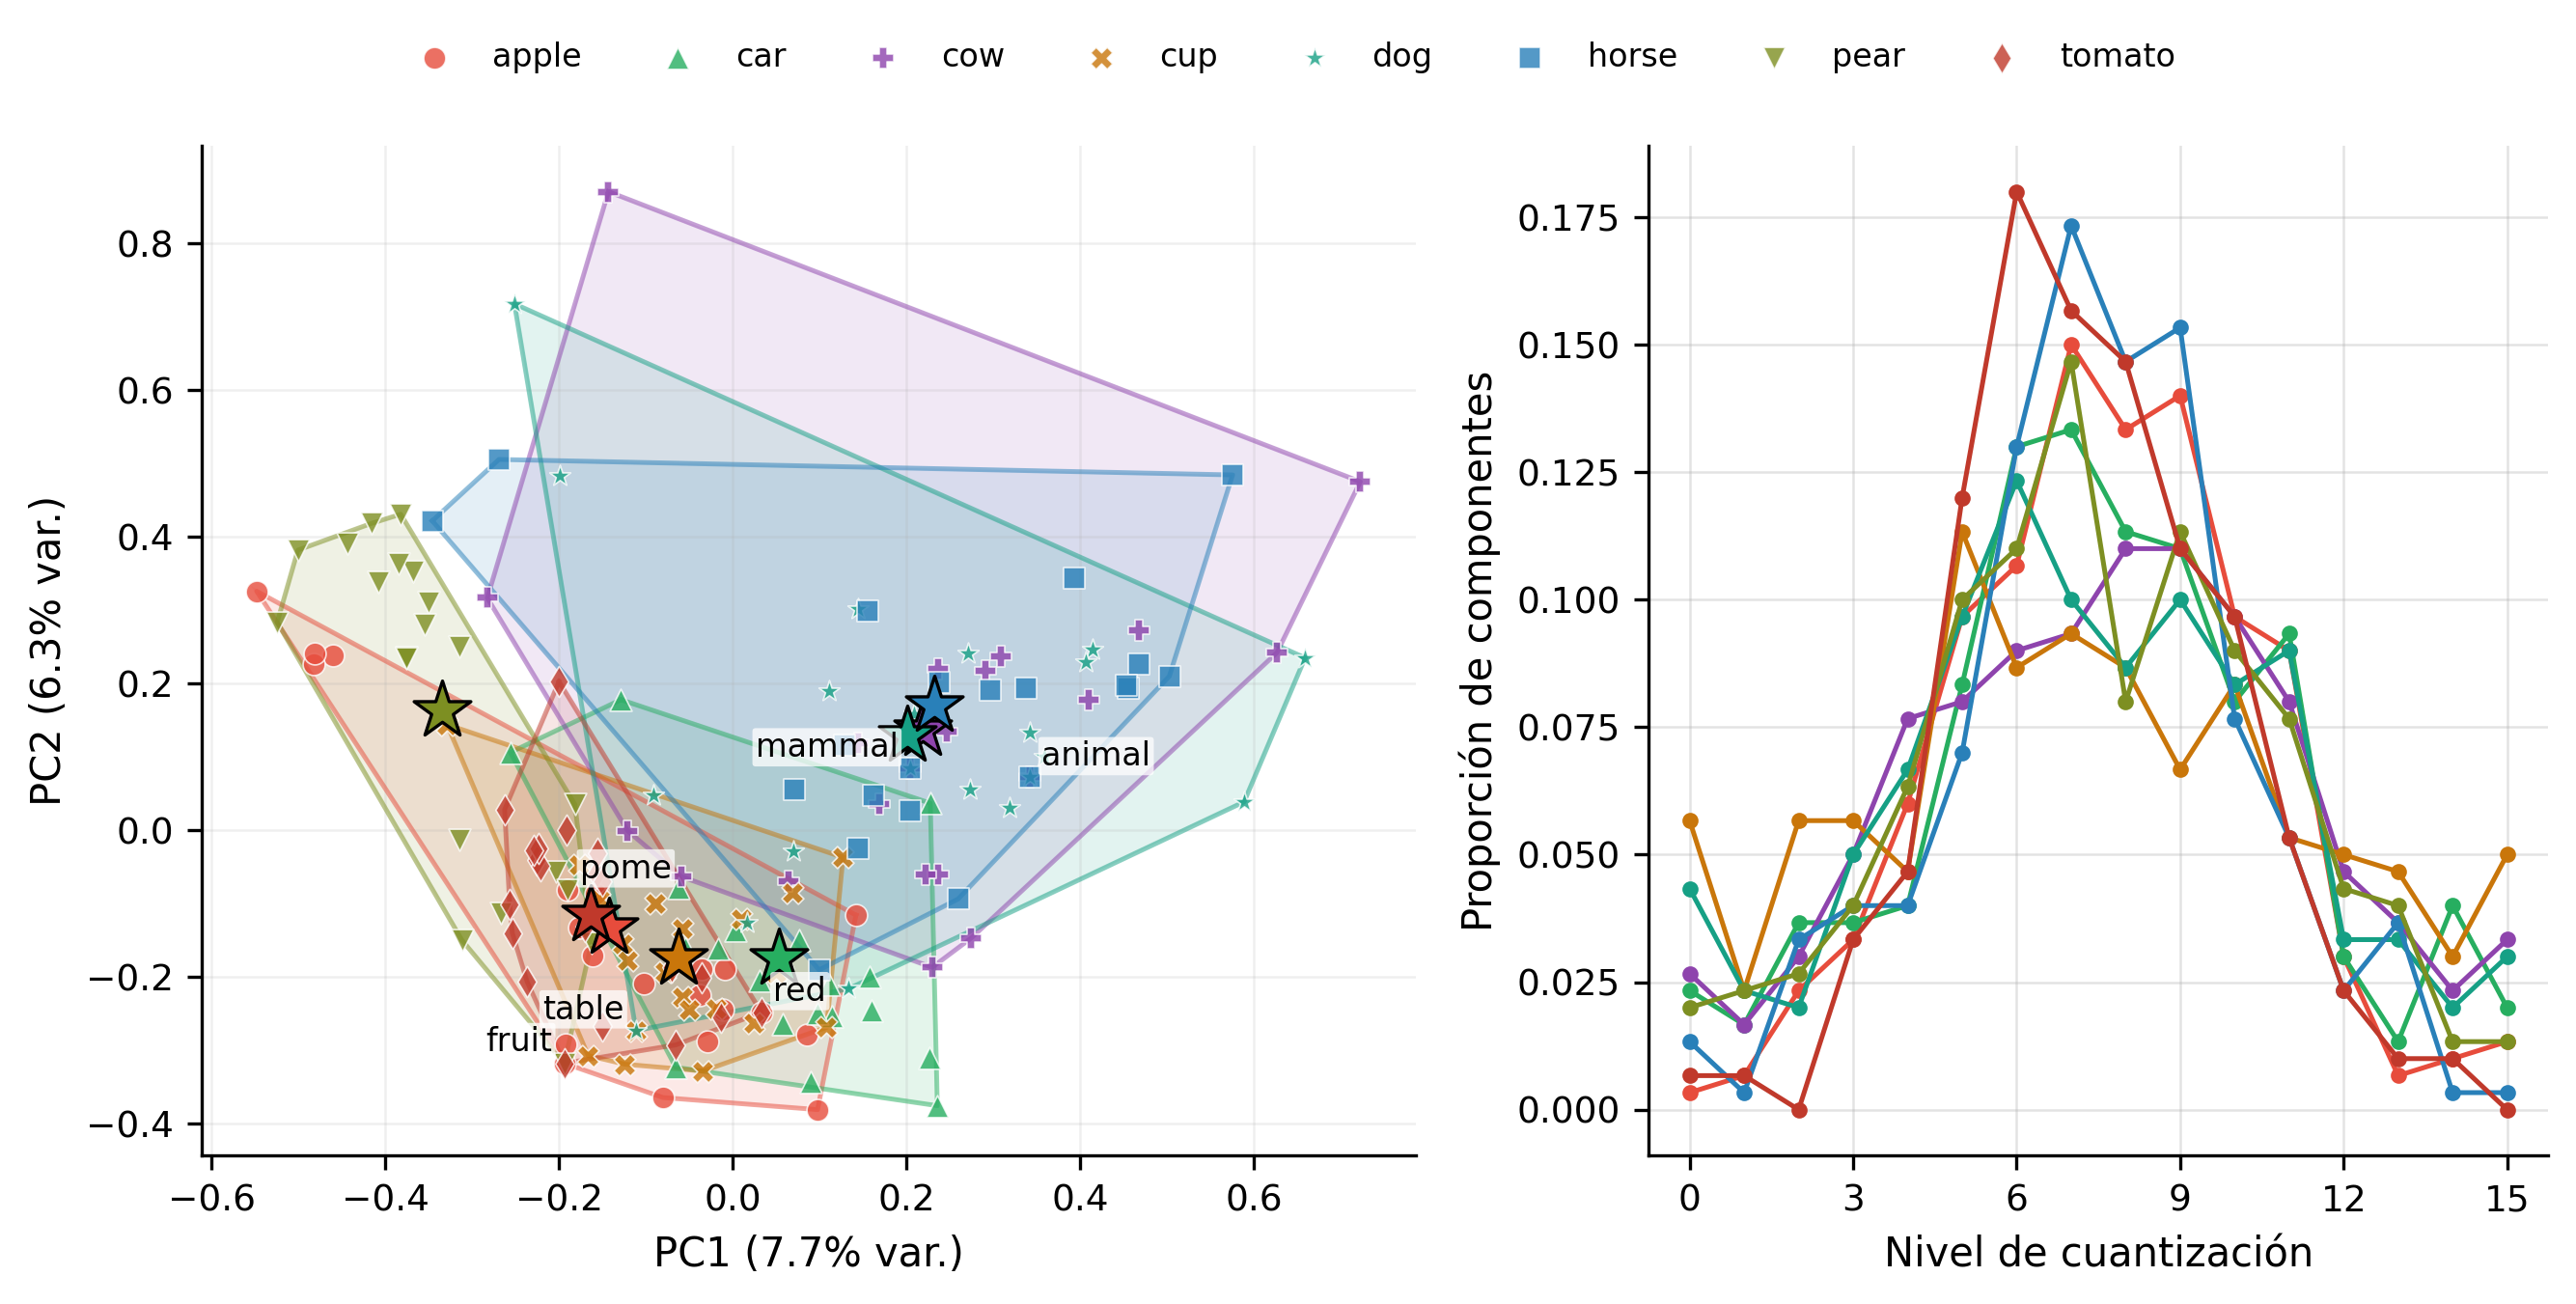
\includegraphics[width=\textwidth]{fig11_semantic_space.png}
    \caption[Espacio semántico de las etiquetas de llenado]{Espacio semántico de las etiquetas de llenado de las ocho clases (vectores
    fastText del vocabulario de la Sección~\ref{sec:pipeline-semantico}).
    Izquierda: proyección en las dos primeras componentes principales (PCA, por sus
    siglas en inglés), con la envolvente y el centroide (estrella) de cada clase; se rotulan solo las etiquetas que comparten dos o tres clases (\textit{fruit},
    \textit{pome}, \textit{red}, \textit{animal}, \textit{mammal} y \textit{table}).
    Derecha: proporción de las 300 componentes que cae en cada uno de los 16 niveles de
    la cuantización por magnitud, para la etiqueta con el nombre de cada clase.}
    \label{fig:espacio-semantico}
\end{figure}

\paragraph{Procesamiento de consultas con spaCy.}
Las consultas en lenguaje natural se procesan con spaCy~3.8.14 y su modelo
\texttt{en\_core\_web\_sm}~3.8.0~\cite{honnibal2020spacy}: se
lematizan, se conservan los tokens de categoría gramatical \texttt{NOUN}, \texttt{ADJ}
o \texttt{PROPN}, se eliminan las palabras vacías y cada token se conserva una sola vez,
en su orden.
Un \emph{rescate léxico} recupera un token que el etiquetador gramatical
descartó si, aislado, se etiqueta como \texttt{NOUN}, \texttt{ADJ} o \texttt{PROPN}, o
si es una etiqueta registrada en las memorias; este segundo criterio solo \emph{admite}
pistas, nunca descarta ninguna.
El rescate corrige errores del etiquetador en frases nominales cortas (p.\ ej.\
\texttt{pear} etiquetado como verbo en «a bosc pear\ldots»), que de otro modo
quitarían la pista más distintiva de la consulta.
Sobre el banco completo, la regla cambia el resultado de 46 consultas.
Con el rescate aciertan 43 (93.5\,\%); sin él aciertan 33 (71.7\,\%) y cuatro se
rechazan.
La diferencia es de diez aciertos (21.7 puntos).
Los diez cambios de ganador van todos hacia la clase correcta, y los tokens rescatados
con más frecuencia son \texttt{bark}, \texttt{riding}, \texttt{drink}, \texttt{canine}
y \texttt{drive}.
La regla no decide el ganador, que sale de la proyección con compuerta de las memorias, pero
sí decide qué tokens entran como pista, con un criterio tomado del vocabulario que llenó
las memorias; por eso se reporta con su efecto medido (limitación (h),
Sección~\ref{sec:limitaciones}).

\paragraph{Representación de tokens, sin filtro de vocabulario.}
El vocabulario de ConceptNet sirve para \emph{llenar} las memorias, no para decidir qué
consultas son conocidas.
Cada token de la consulta se convierte en una pista vectorial tomando su vector del
modelo fastText completo, exista o no como etiqueta de ConceptNet.
No se aplica ningún filtro de pertenencia léxica. Una vez obtenida la pista, es la
propia memoria la que, mediante el reconocimiento y la contención, decide si
hay soporte o se rechaza (puntuación cero).
Solo queda fuera lo que no es representable. Un token sin vector fastText real no genera
pista y, por tanto, no llega a la memoria.

% ---------------------------------------------------------------
\subsubsection{Percepción visual: codificador ResNet18}
\label{sec:percepcion}

Para obtener representaciones latentes de las imágenes se entrenó sobre las ocho clases
un autocodificador convolucional con codificador basado en ResNet18~\cite{he2016resnet},
inicializado con los pesos de ImageNet.
El espacio latente tiene dimensión 64.
La pérdida suma el error cuadrático medio de reconstrucción (MSE) y una entropía
cruzada de clasificación (CE) con peso 0.1; la cabeza clasificadora solo guía el
entrenamiento del codificador y \textbf{no participa} en el enrutamiento ni en la
recuperación del sistema de memorias.
El entrenamiento es \emph{determinista} (semilla 42 en \texttt{torch}, \texttt{numpy} y
\texttt{random}, con cuDNN determinista), de modo que una réplica desde cero es
reproducible; el codificador alcanza una raíz del error cuadrático medio (RMSE) de 0.110 y
una precisión de la cabeza auxiliar del 99.7\,\%.
No hay partición de validación separada, y el punto de control se elige por RMSE mínimo
sobre el propio conjunto de prueba (una evaluación cada 10 épocas, es decir, cinco
candidatos), así que el espacio latente con el que se evalúa el hemisferio visual se
eligió con información de ese conjunto (limitación (g), Sección~\ref{sec:limitaciones}).
Los vectores latentes se cuantizaron a $m = 32$ niveles con una normalización global
min-max con un margen del 10\,\%.
El rango se calculó solo sobre las 200 imágenes de llenado de cada clase, con la
original, el espejo y las rotaciones de $\pm 12^{\circ}$ de cada una (6400 latentes), y
se guardó con el modelo.
Lo que cae fuera del rango se recorta al nivel extremo.
Esta cuantización global evita que la escala relativa entre clases afecte la codificación.

Antes de llegar a la memoria, toda percepción pasa un \textbf{umbral de energía}: si
la norma de su latente continuo es menor que $\tau = 16.61$, se rechaza sin consultar
la memoria.
El umbral $\tau$ es el mínimo de esa norma sobre las 1600 imágenes originales del llenado
(18.45) con un margen del 10\,\%. Hace falta porque el codificador lleva las entradas sin
estructura (gris uniforme, desenfoque, contraste nulo) cerca del origen, donde la
memoria les da soporte (experimento~14\footnote{Los
experimentos se citan con el número de su carpeta en \texttt{results/}, donde están el
protocolo y las tablas completas: 10 (tolerancia $\xi$ con directorios
perspectivales), 11 (comparación con una sola EHAM), 13 (variantes por percepción), 14
(umbral de energía), 15 (árbitro por contenido), 16 (objetos nuevos) y 19 (codificador
de ImageNet sin reentrenar).},
Sección~\ref{sec:hemisferio-visual}).
Es un criterio previo a la EAM y tiene costo: no rechaza ninguna imagen del llenado,
pero sí 1 de las 1024 de la formación visual y 4 de las 656 de prueba, cuatro vistas de vaca
que el directorio enrutaba bien y que su especialista aceptaba.

% ---------------------------------------------------------------
\subsubsection{Banco de evaluación semántica}
\label{sec:banco}

Se construyó un banco de \textbf{411 consultas} en lenguaje natural con su clase
correcta conocida, aproximadamente 50 por dominio,
presentadas de forma intercalada.
El banco está alineado con el vocabulario de llenado.
De las 411 consultas, 402 contienen una palabra del vocabulario de su clase, 367 una
palabra que solo está en ese vocabulario y 208 el nombre de la clase.\footnote{Reanálisis
del banco, \texttt{results/reanalisis\_jurado/salida.md}, tabla M3.1. Una palabra cuenta
si aparece como palabra de la consulta, también en plural; el sistema tokeniza con
spaCy, así que la cuenta es una aproximación.}
Las consultas varían en longitud y vocabulario (p.\ ej.\ «a crunchy red apple»,
«a barking domestic pet», «a mug for liquid») y cubren tanto descripciones
directas como perifrásticas; las clases con léxico compartido (\texttt{pear},
\texttt{tomato}) incluyen consultas con contenido \emph{distintivo}
(«a bosc pear with brown skin», «a tomato on the vine»), en las que quien pregunta
aporta las señas del dominio.
Los experimentos de protocolo completo (Secciones~\ref{sec:proto-completo}
a~\ref{sec:formacion}) usan las primeras 80 consultas (10 por clase), y el estudio de
calibración (Sección~\ref{sec:calibracion}), hasta 400.
Otros tres bancos se usan una sola vez.
La Sección~\ref{sec:proto-completo} usa las 16 consultas de referencia del sistema (dos
por dominio) y 12 consultas representables que describen objetos fuera de los ocho
dominios.
La comparación con una sola EHAM (Sección~\ref{sec:eham-unica}) usa una partición del
banco, en la que las primeras 30 consultas de cada clase forman los directorios y las 171
restantes quedan reservadas para evaluar, más 40 consultas fuera de dominio: las 12
anteriores y 28 de objetos y escenas de categorías ausentes de ETH-80, sin palabras del
vocabulario de etiquetas.
Las reservadas son la cola de la lista de cada clase, no una muestra al azar, y no
representan al banco.
El 87.7\,\% de ellas trae el nombre de su clase, frente al 24.2\,\% de las 240 de
formación, el 13.8\,\% de las 80 primeras y el 49.8\,\% de las 400 de la
calibración.\footnote{Reanálisis del banco, tabla M3.1.}

% ---------------------------------------------------------------
\subsubsection{Parámetros de la EAM}
\label{sec:parametros}

Los parámetros de la EAM se fijaron en $\iota = 0$, $\kappa = 0$, $\sigma = 0.1$ y
tolerancia de reconocimiento $\xi = 0$, iguales en las memorias de contenido y en los
directorios de texto y visuales.
Estos valores siguen el modelo W-EAM y su extensión heteroasociativa
(Sección~\ref{sec:marco_teorico}).
La propia línea W-EAM ha mostrado que estos hiperparámetros admiten optimización
automática multiobjetivo \cite{lopez2025hyperopt}; aquí se fijan por barrido directo,
cuya justificación experimental se presenta en la Sección~\ref{sec:param-iota-kappa}
(barrido $\iota \times \kappa$) y en la Sección~\ref{sec:hemisferio-visual}
($\xi$ visual).

Todas las proyecciones usan los pesos por característica de la ecuación~\eqref{eq:pesos},
calculados sobre la propia memoria: en la de contenido, sobre la lectura del dominio de
la pista (ecuación~\eqref{eq:marginal}); en los directorios, sobre su relación (cuántas
veces se registró cada valor en cada característica, lo mismo que daría una memoria
homoasociativa llenada con las mismas pistas).
Los pesos solo cambian magnitudes; la contención, y con ella la aceptación y el rechazo,
no depende de ellos.

% ---------------------------------------------------------------
\subsubsection{Auditoría de trazabilidad}
\label{sec:auditoria}

La auditoría de trazabilidad comprueba que las operaciones de memoria son las de la
implementación de referencia, que el vocabulario no contiene vectores sintéticos y que
la clase correcta no entra al circuito de decisión:
\begin{itemize}
    \item El vocabulario no contiene vectores sintéticos: una etiqueta sin vector fastText
    real queda fuera del llenado, y la escala global $S = 0.1881$ se calcula solo sobre
    vectores reales.
    \item El código de las memorias de Pineda y Morales es idéntico byte a byte al
    original, salvo una condición que evita cargar sus clasificadores y no toca ninguna
    operación de memoria.
    \item La clase correcta de cada consulta se usa solo para calcular métricas, nunca
    dentro del circuito de decisión.
\end{itemize}
Fuera de las memorias quedan cuatro operaciones, declaradas en la arquitectura: la suma
de las puntuaciones sobre los tokens, la lectura normalizada, el umbral de energía $\tau$
y el rescate léxico.
Todos los números reportados salen de corridas de este sistema, con sus tablas en
\texttt{results/}.

% ---------------------------------------------------------------
\subsubsection{Organización del experimento}
\label{sec:organizacion}

Los resultados de la Sección~\ref{sec:resultados} siguen el orden de las fases.
Los estudios de la fase 3 son, en este orden, el protocolo completo, los parámetros
propios $\iota \times \kappa$, la formación del directorio y la capacidad de llenado
(Secciones~\ref{sec:proto-completo} a~\ref{sec:capacidad}); el hemisferio visual
(Sección~\ref{sec:hemisferio-visual}); la generalización a objetos nuevos
(Sección~\ref{sec:objetos-nuevos}); el hemisferio visual con un codificador entrenado
sin la pérdida de clase (Sección~\ref{sec:codificador-sin-clase}); la comparación con
una sola EHAM (Sección~\ref{sec:eham-unica}); la comparación de una EHAM de dos clases
con una de ocho; la verificación de una sola memoria de contenido por módulo
(Sección~\ref{sec:una-memoria}); la comparación con decisores sin memoria asociativa
sobre los mismos vectores (Sección~\ref{sec:lineas-base}), y el costo computacional de
la reproducción completa (Sección~\ref{sec:costo}).
Las dos calibraciones pertenecen a la fase 2 (Sección~\ref{fase2:lectura}).

La comparación de dos clases contra ocho (experimento~12) recorre los 28 pares de
clases.
Para cada par, una EHAM llenada solo con esas dos clases, con 200 imágenes por clase y
el llenado de la comparación con una sola EHAM, responde las consultas reservadas de
las dos clases, con cinco semillas y tres sorteos.
Sobre las mismas consultas y semillas responden también el especialista y la EHAM de
ocho clases.
La brecha de fidelidad mide cuánto más lejos de la instancia real más cercana queda el
recuerdo de cada EHAM que el del especialista.
De cada par se mide además el solapamiento de los soportes de las dos clases (Jaccard
medio por coordenada), en el lado de las etiquetas y en el latente.
La predicción registrada antes de correr era que la brecha crece con el solapamiento.

En las dos calibraciones, el protocolo completo, el barrido $\iota \times \kappa$ y la
formación del directorio, cada transacción de texto se registra en un solo
\emph{directorio compartido}, igual al registro completo del TME.
Los directorios perspectivales de la Sección~\ref{sec:componentes}, en los que solo
registran el módulo de entrada y el ganador, se usan en el hemisferio visual y en la
comparación con una sola EHAM.

% ---------------------------------------------------------------
\subsection{Fase 4: experimentos de propiedades}
\label{fase4:propiedades}

Con el sistema de ocho módulos se diseñaron experimentos que preguntan qué hace el
sistema además de acertar.
Se agrupan en seis temas.
Los temas de reconocer y recordar (envolvente, contención y familiaridad) y de los
límites del rechazo usan estudios de la fase 3 ya descritos: los objetos nuevos, el
codificador sin pérdida de clase, el umbral de energía, la verificación de una sola
memoria de contenido y la sonda de rechazo.
Los otros cuatro temas tienen experimentos propios, que se describen abajo; los
resultados están en la Sección~\ref{sec:resultados}.

Varios de estos experimentos estudian el directorio y no la elección del ganador.
En ellos el directorio se forma con la clase real como ganador de cada transacción, para
separar lo que el directorio guarda del acierto de la fase temprana.
Los experimentos 7 a 10 se corrieron antes de que el sistema adoptara los directorios
perspectivales y una sola memoria de contenido, con el directorio visual llenado sin
variantes.
En el 8 y el 9 todos los módulos registran todas las transacciones, sus directorios son
idénticos y las memorias homoasociativas están al lado de la heteroasociativa; el 10
parte de ese registro para medir directorios que divergen.
Los experimentos 7, 8 y 10 miden sobre todo directorios.
En el 9 el sustituto reconoce y evoca con sus memorias homoasociativas, que el sistema
final ya no tiene, y por eso se reporta con esa salvedad.
Ninguno da cifras del sistema final.

\paragraph{El directorio como índice.}
En el experimento~7, un solo directorio recibe pistas de texto y de imagen, para ver si
forma una representación compartida de las dos modalidades.
Su relación tiene 364 características, 300 de texto (recuantizadas a 32 niveles con la
misma escala global) y 64 del latente.
La mitad que falta en cada pista se registra y se consulta como valor indefinido, que la
proyección salta.
El directorio se forma de tres maneras, solo con texto, solo con imagen y con pares de
texto e imagen, y se compara con dos directorios separados.
El texto usa las 80 consultas de los estudios de protocolo, evaluadas dentro de muestra.
La imagen se forma con las 128 imágenes de entrenamiento por clase de la formación
visual y se evalúa con 20 imágenes de prueba por clase.
La lectura es B1.

El experimento~8 lee el directorio en el sentido inverso, de la identidad de un módulo a
una pista en su dominio, con la recuperación $\beta$ desde la derecha.
Se comparan tres respuestas para cada clase: la de la memoria de contenido del
especialista con su propia etiqueta (lo vivido), la del directorio con el dominio propio
y la del directorio con un dominio ajeno que el módulo presenció.
Las juzgan el clasificador latente del codificador y el vecino más cercano entre las
6400 instancias reales del llenado.
Dos barridos completan el diseño, uno sobre cuántas transacciones ajenas presenció el
módulo, de 0 a 128, y otro sobre cuántos registros tiene el directorio, de 1 a 800 por
módulo.
Un control pregunta por identidades que ningún módulo tiene.

\paragraph{La perspectiva y la pérdida de un miembro.}
El experimento~10 compara un grupo cuyos módulos solo registran lo que presencian con un
registro único del grupo, el pizarrón.
El ganador siempre registra lo suyo.
Un módulo que no ganó registra la transacción de dos maneras según la condición: al
azar con probabilidad $f \in \{0, 1/64, 1/32, 1/16, 1/8, 1/4, 1/2, 1\}$, con tres
semillas, o solo si el ganador está a distancia $r \le 4$ en un anillo de los ocho
módulos.
Cada consulta entra por cada uno de los ocho módulos y se resuelve con cuatro
protocolos:
\begin{itemize}
    \item directo, en el que el módulo de entrada consulta su directorio y rechaza si no
    hay soporte;
    \item encadenado, en el que la consulta sin soporte pasa a los módulos conocidos, por
    orden de familiaridad, hasta que alguno tiene soporte;
    \item agregado, en el que el módulo de entrada suma las puntuaciones normalizadas de
    todos sus conocidos y elige la mayor;
    \item pizarrón, el directorio único con todos los registros, como referencia.
\end{itemize}
El texto se forma con 30 consultas por clase (240) y se evalúa también con las 171
reservadas; la imagen se forma con 128 latentes de entrenamiento por clase y se evalúa
con 20 de prueba por clase, con $\xi = 0$.
Además del acierto, se miden los saltos del encadenado y la divergencia de Jaccard entre
los soportes de cada par de directorios.

En el experimento~9 se quita un módulo $k$, y las consultas de su dominio entran por un
sobreviviente, que las enruta como en la fase madura.
Sobre las consultas que el directorio sigue mandando a $k$ se comparan tres políticas
del grupo sin $k$:
\begin{itemize}
    \item sustitución, en la que responde con su propio contenido el sobreviviente de
    mayor puntuación en el directorio;
    \item descripción, en la que el sobreviviente responde con lo que presenció de $k$,
    leyendo su directorio en el sentido inverso del experimento~8;
    \item rechazo, no responder.
\end{itemize}
La referencia es la respuesta de $k$ presente.
Se usan las 411 consultas del banco, con tres repeticiones porque la recuperación
muestrea, y 10 imágenes de prueba por clase.
En el sentido texto $\to$ imagen la respuesta se juzga por su clase y por su distancia
a la instancia real más cercana del dominio perdido.
En el sentido imagen $\to$ texto acierta si alguna de las tres palabras evocadas
pertenece al vocabulario de ese dominio.
Una sonda aparte mide cuánto del dominio de $k$ reconoce el especialista frente a un
módulo que no lo es.

\paragraph{El tamaño y la partición.}
Las dos mediciones controladas de este tema son la comparación con una sola EHAM y la
de dos clases contra ocho, descritas en la Sección~\ref{sec:organizacion}.
La lectura por el principio de tamaño (experimento~22) está con la fase 2
(Sección~\ref{fase2:lectura}).

\paragraph{La imagen y la palabra.}
La evocación de dominio cuenta como acierto que una de tres palabras sea de la clase.
Para saber si la evocación devuelve una palabra específica, el experimento~17 usa tres
condiciones:
\begin{itemize}
    \item A, los modelos oficiales con top-1 en lugar de top-3, sobre las mismas 118
    imágenes de prueba de la evocación de dominio y con tres recuerdos por imagen;
    \item B, un llenado nuevo en el que todas las vistas del objeto $k$ de cada clase se
    registran con la $k$-ésima palabra exclusiva del vocabulario de la clase, con 200
    imágenes y 16 variantes por clase, donde el azar es del 10\,\%;
    \item C, el color como palabra, con 80 objetos etiquetados a mano por su color
    dominante y una paleta de ocho colores.
\end{itemize}
Las respuestas se leen de cuatro formas: la recuperación oficial con el vecino por
coseno, el prototipo (el valor más probable de cada coordenada), el soporte (la
probabilidad media que la proyección da a cada palabra candidata) y el soporte dividido
entre el de la memoria completa, que es el análogo de B1 y se fijó antes de correr.
Se evalúa en el módulo de la clase verdadera.

El experimento~18 asocia cada imagen con una característica que el objeto tiene, con
una memoria heteroasociativa por eje y clase: patrón (liso, con manchas o decorado) en
\texttt{cow}, \texttt{horse}, \texttt{dog} y \texttt{cup}; techo (convertible o fijo)
en \texttt{car}, y pelo (rizado o liso) en \texttt{dog}.
Las etiquetas se pusieron a mano por objeto y solo entran los objetos claros en cada
eje.
Cada memoria se llena con 200 vistas en 16 variantes, se evalúa con vistas nuevas de
objetos conocidos y con objetos nuevos en una validación \textit{leave-one-object-out}
de 52 pliegues.
Las lecturas son las de soporte del experimento~17, que eligen entre las palabras del
eje y no ejecutan un recuerdo.
Se compara con un $k$-vecinos sobre los mismos latentes y sobre los rasgos de un ResNet18
de ImageNet sin ajustar.

Con el experimento~19 se mide qué gana el especialista y qué pierde el índice cuando la
percepción conserva el detalle dentro de la clase.
Cambia el codificador por un ResNet18 de ImageNet congelado y un análisis de componentes
principales a 64 dimensiones, ajustado solo con las 2624 imágenes de entrenamiento.
Con ese codificador se corren de nuevo el llenado, las dos fases, el hemisferio visual,
los objetos nuevos (diez pliegues) y el experimento~18.
Se corrió en una copia del sistema anterior a la memoria de contenido única.

% ---------------------------------------------------------------
\subsection{Fase 5: laboratorio en tiempo real}
\label{fase5:laboratorio}

La fase 5 conectó el sistema a un micrófono y a una cámara para ver si funciona con
entradas continuas.
Usa la versión v5 del sistema, de julio de 2026, con ocho módulos que llevan tres
memorias de contenido cada uno (la heteroasociativa y dos homoasociativas), un
directorio de texto y un directorio visual, más el TME.
No es la arquitectura final, y no hay ninguna corrida con ella.
El laboratorio carga los modelos en modo de solo lectura y corre en una ventana de
Python con tres hilos, uno para el audio, uno para la visión y uno para la interfaz.

\paragraph{Voz.}
El micrófono entrega audio a 16\,kHz en un canal, en bloques de 30\,ms.
Un detector de voz propio compara la energía de cada bloque con un piso de ruido que se
adapta en los silencios, y cierra la frase tras unos 600\,ms de silencio.
La frase cerrada la transcribe Whisper \textit{small}, con la biblioteca
\textit{faster-whisper} en la GPU y respaldo en la CPU.
La transcripción usa el modo de traducción: se puede hablar en español o en inglés, y
sale texto en inglés, el idioma del vocabulario de fastText.
Mientras se habla aparecen subtítulos parciales.
La frase transcrita entra al hemisferio textual en uno de dos modos.
En el temprano, el TME la difunde a los ocho módulos y la registra en un directorio de
sesión, que vive en memoria y no toca los modelos guardados.
En el maduro, el TME está apagado, y el módulo de entrada consulta su directorio con la
lectura B1 y redirige al especialista o rechaza.
Tras el enrutamiento, la memoria del destino evoca una imagen en un hilo aparte, que el
decodificador dibuja sin detener el video ni la escucha.

\paragraph{Cámara.}
Cada 250\,ms, aproximadamente, se toma el recuadro central del cuadro, que por omisión
ocupa el 55\,\% del lado menor, y se pasa a $128 \times 128$ píxeles al codificador.
El latente cuantizado consulta el directorio visual del módulo de entrada con la lectura
tolerante de la versión v5, y la etiqueta que se muestra es la mayoría de los últimos
cinco análisis.
Si el directorio rechaza el cuadro, se intenta otra vez con los momentos de color RGB
normalizados a los de ETH-80, y si lo rechaza de nuevo, la interfaz muestra el candidato
más cercano.
Como el segundo intento solo corre tras un rechazo, no cambia las decisiones sobre los
cuadros que el directorio ya aceptaba.

\paragraph{Pruebas.}
Whisper corrió en una GPU NVIDIA RTX 2050, y el codificador y las memorias, en la CPU.
La cadena de voz de punta a punta se probó con un archivo WAV inyectado por el camino
del micrófono, con la frase «Farm animal that gives milk», en los dos modos y con dos
módulos de entrada.
Se midieron una vez la latencia de la transcripción y la del enrutamiento, el tiempo de
análisis de un cuadro y la tasa de cuadros de la interfaz.
La política de color se probó en simulación, sobre 24 imágenes de prueba de ETH-80 en
tres condiciones: limpias, con un tono grisáceo medio y con uno fuerte.
Con la cámara física se mostraron imágenes de ETH-80 en la pantalla de un teléfono y en
una hoja impresa con 16 imágenes, y se pasó por el directorio visual un cuadro gris sin
objeto, ajeno a ETH-80 (\texttt{selftest\_frame.png}).
Las mediciones son del 16 al 18 de julio de 2026 y no quedó registro crudo de ellas;
lo que se conserva está en \texttt{results/mundo\_real/}.
No se midieron la tasa de error de la transcripción, el acierto del enrutamiento con voz
ni el acierto con la cámara física.
Por eso la fase 5 es una demostración de integración.
Las consultas habladas en español y las imágenes de otro origen quedan fuera del alcance
de la evaluación del sistema.

\section{Resultados}
\label{sec:resultados}

Las secciones siguen el orden de la Sección~\ref{sec:organizacion}.
Salvo indicación en contrario, los experimentos usan los parámetros de la
Sección~\ref{sec:parametros}, y todos los números son trazables a corridas del sistema
actual (Sección~\ref{sec:auditoria}).

% ---------------------------------------------------------------
\subsection{Calibración del directorio a ocho módulos}
\label{sec:calibracion}

La calibración mide cómo debe leerse el directorio para que el enrutamiento maduro sea
confiable.
Se compararon nueve condiciones: la lectura cruda (A), dos normalizaciones por el conteo
de registros de cada módulo (B1, B2) y seis que actúan sobre otra cosa: un tope de
registros por módulo (C), consultas balanceadas (D), la cuantización (E32, E64), el
vocabulario (F) y la combinación de D, B1 y F (G).
Cada una se evaluó sobre el banco de 411 consultas, con $N \in \{50, 100, 200, 400\}$
consultas para formar el directorio y 5 semillas por celda.
La Tabla~\ref{tab:calibracion} da los resultados en $N = 400$; la
Figura~\ref{fig:mature-vs-n} muestra cómo crece la precisión madura con $N$, y la
Figura~\ref{fig:heatmap-condicion} da los mismos valores como mapa de calor.

En este estudio, como en el protocolo completo y en la curva de formación, la fase
madura se evalúa sobre las mismas $N$ consultas cuyos tokens formaron el directorio:
mide si el directorio reproduce lo que registró, no si generaliza a consultas nuevas.
Sobre 171 consultas reservadas, el protocolo transactivo del experimento 11 enruta
correctamente el 97.0\% con 200 imágenes por clase (Sección~\ref{sec:eham-unica}).

\begin{table}[H]
    \centering
    \caption{Precisión bajo distintas condiciones de lectura del directorio
    ($N = 400$, media de 5 semillas, 400 consultas del banco de 411).
    La precisión temprana no depende de la lectura del directorio, por lo que solo
    varía en las condiciones que alteran las consultas (D, G).
    F coincide con A: el vocabulario por masa asociativa no contiene las etiquetas
    polisémicas (las de Apple~Inc.) que la depuración quitaría.}
    \label{tab:calibracion}
    \small
    \setlength{\tabcolsep}{4pt}
    \begin{tabular}{llccc}
        \toprule
        Condición & Descripción & Temprana (\%) & Fidelidad (\%) & Madura (\%) \\
        \midrule
        A (cruda)  & Puntuación de activación sin normalizar        & 90.0 & 90.5 & 85.2 \\
        B1         & División entre conteo de registros por módulo  & 90.0 & 95.8 & \textbf{93.0} \\
        B2         & División entre raíz cuadrada del conteo        & 90.0 & 95.2 & 91.8 \\
        C          & Tope de registros por módulo                   & 90.0 & 91.2 & 88.0 \\
        D          & Consultas balanceadas entre clases             & 90.5 & 91.4 & 87.3 \\
        E32        & Cuantización en 32 niveles                     & 90.0 & 92.2 & 88.5 \\
        E64        & Cuantización en 64 niveles                     & 90.0 & 93.0 & 89.8 \\
        F          & Vocabulario depurado ($\equiv$ A)              & 90.0 & 90.5 & 85.2 \\
        G          & D + B1 + F                                     & 90.5 & 95.7 & 93.5 \\
        \bottomrule
    \end{tabular}
\end{table}

\paragraph{B1 es la corrección que no se puede sustituir.}
La lectura cruda del directorio (A) pierde 7.8 puntos frente a la lectura B1 (85.2\%
frente a 93.0\%).
Ninguna de las condiciones que actúan sobre los síntomas del sesgo y no sobre su causa
(B2, C, D, E32, E64) alcanza a B1; la más cercana, B2, queda a 1.2 puntos.
La combinación G supera a B1 por medio punto (93.5\% frente a 93.0\%), menos de lo que
G varía entre semillas (de 93.0 a 93.7\%; B1 da lo mismo con todas): una vez que la
puntuación mide evidencia por registro y no evidencia total, balancear las consultas y
depurar el vocabulario aportan poco.

\begin{figure}[H]
    \centering
    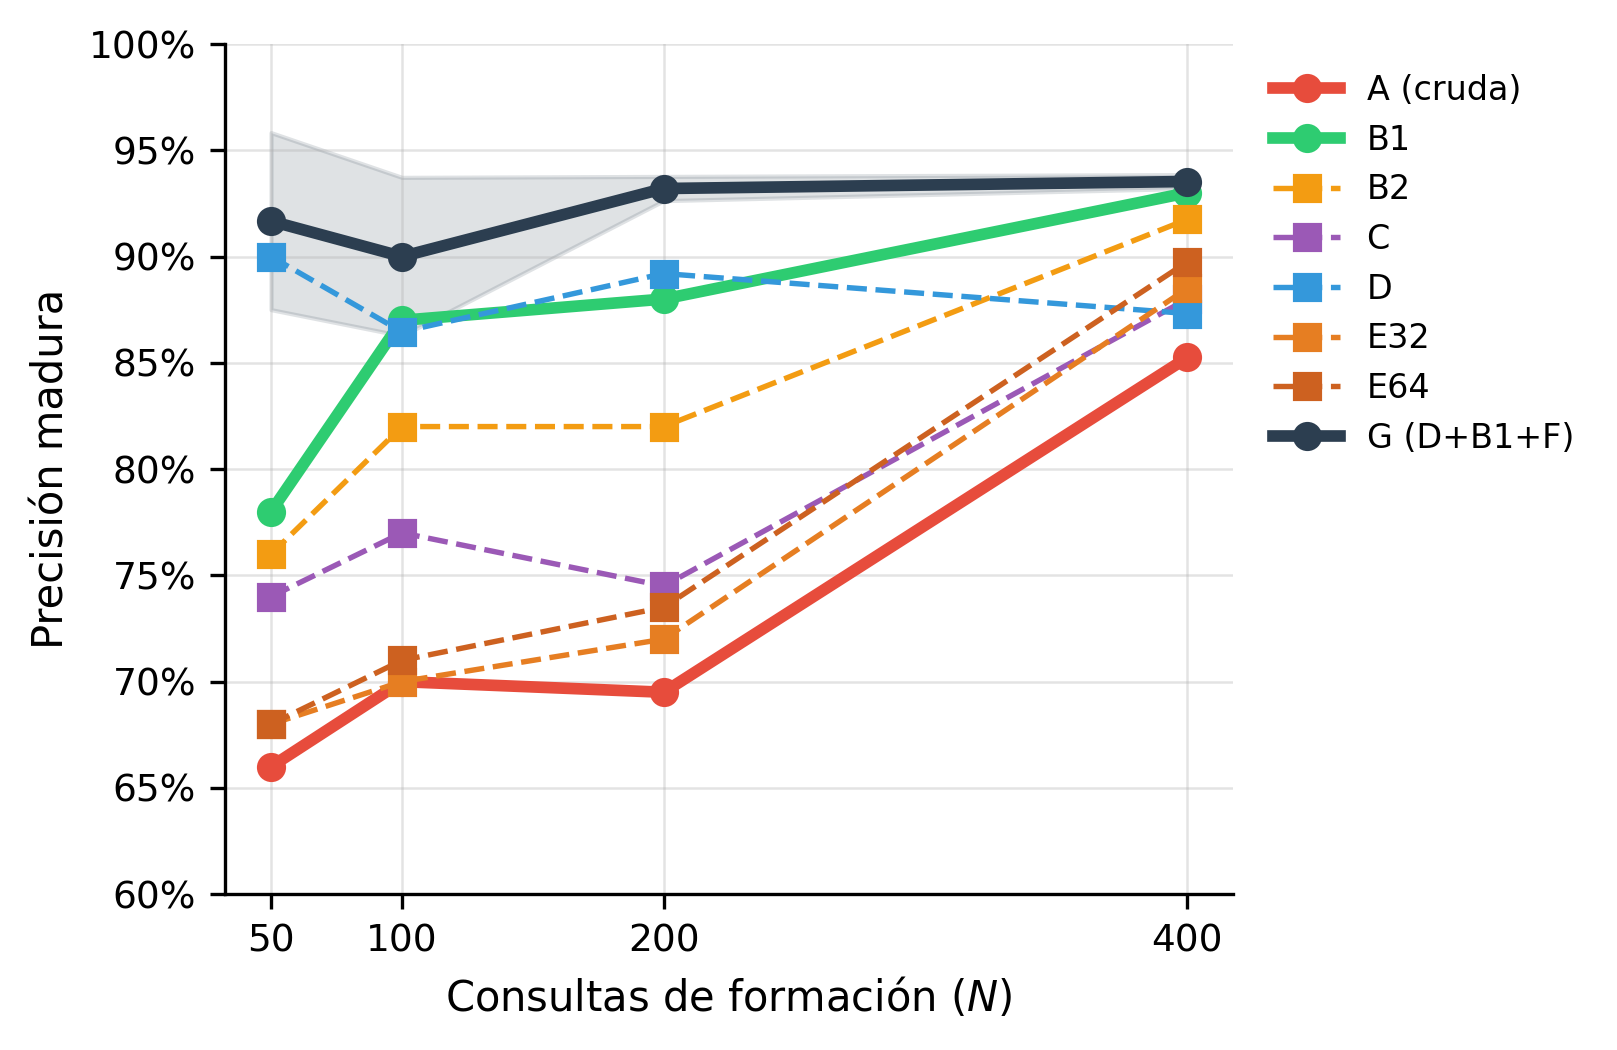
\includegraphics[width=0.9\textwidth]{fig02_mature_accuracy_vs_N.png}
    \caption{Precisión madura en función de $N$ para las condiciones de la
    Tabla~\ref{tab:calibracion} ($N$ consultas del banco de 411, media de 5 semillas; la
    banda es $\pm 1$ desviación estándar de G).
    Entre las condiciones que solo cambian la lectura, B1 es la mejor en todo el rango y
    la cruda (A) queda por debajo.
    G, que además balancea las consultas, queda por encima de B1 en todo el rango; D lo
    supera en $N = 50$ y $200$.
    F coincide con A en todos los puntos y no se dibuja.}
    \label{fig:mature-vs-n}
\end{figure}

\begin{figure}[H]
    \centering
    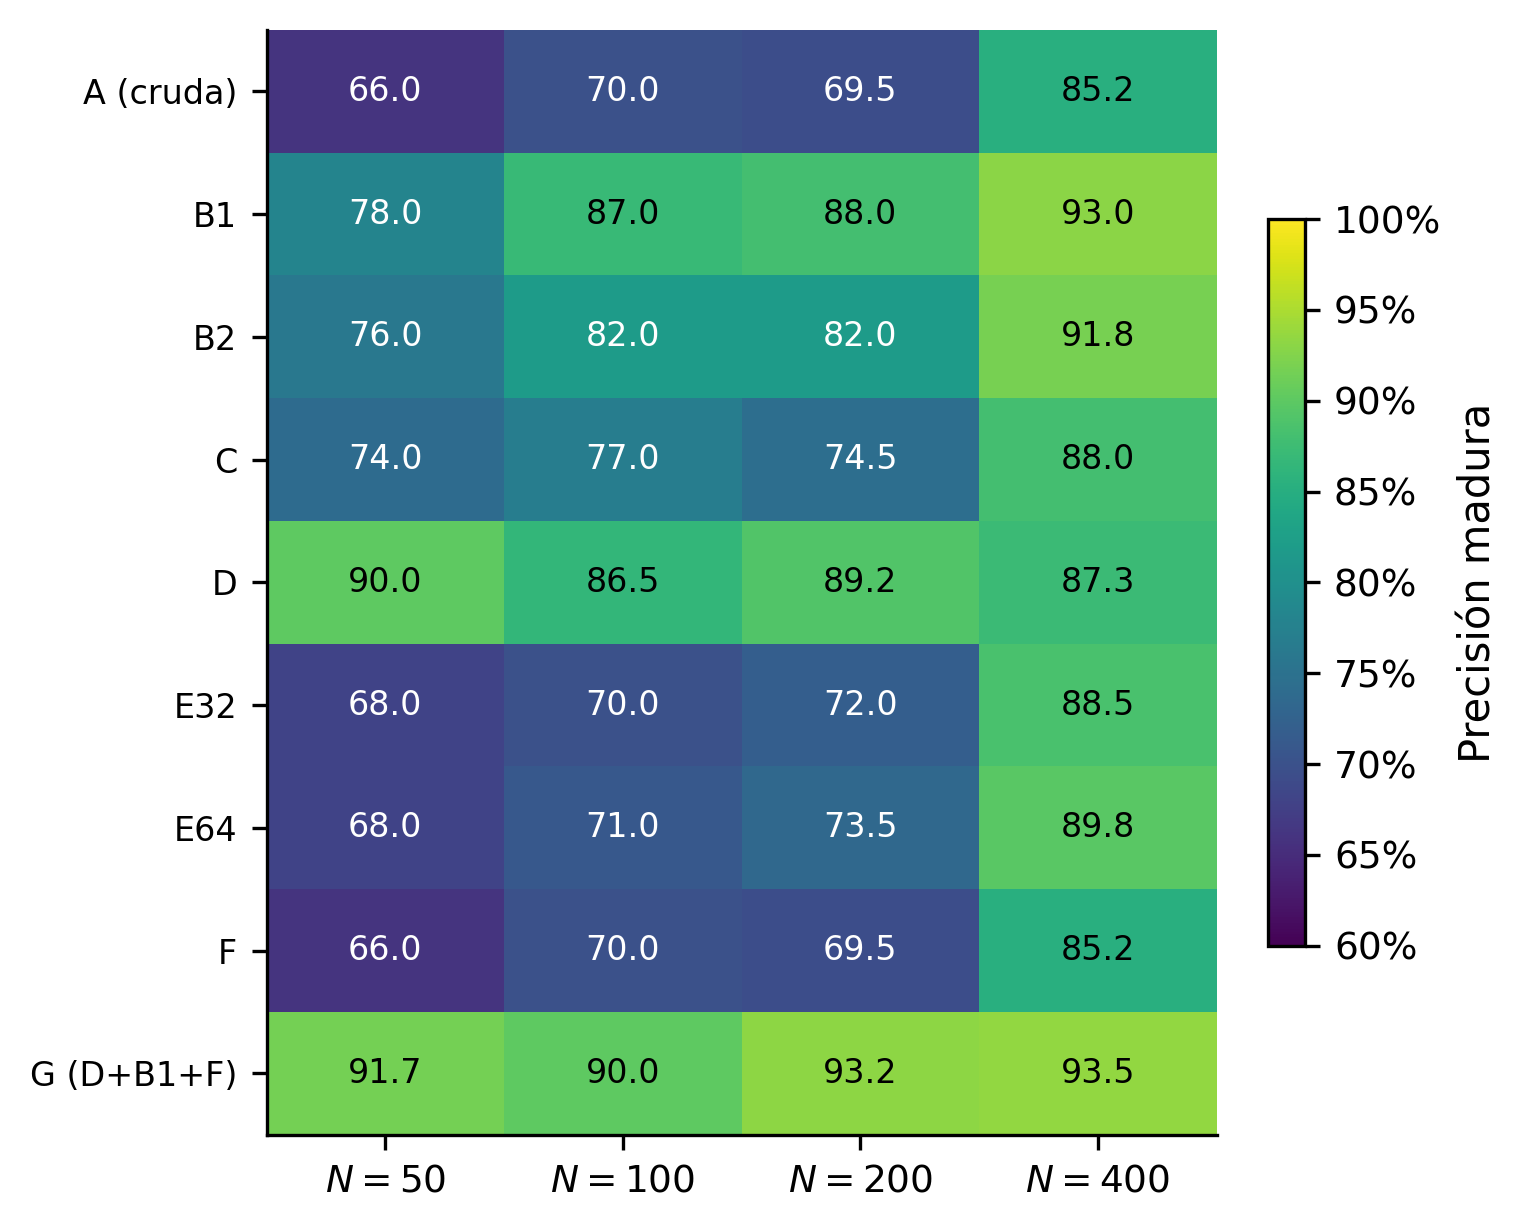
\includegraphics[width=0.75\textwidth]{fig03_heatmap_condition_N.png}
    \caption{Precisión madura (\%) por condición de la Tabla~\ref{tab:calibracion} y
    número de consultas de formación $N$ (mismos datos que la
    Figura~\ref{fig:mature-vs-n}).
    Hasta $N = 200$, A, C, E32, E64 y F quedan entre 66 y 77\%, y B1 sube de 78 a 88\%
    (93\% con $N = 400$); D y G pasan del 86\% en todo el rango.}
    \label{fig:heatmap-condicion}
\end{figure}

\paragraph{Desglose por dominio.}
Con la lectura B1 en $N = 400$, cinco dominios quedan por encima del 90\%
(\texttt{cow}, \texttt{cup} y \texttt{tomato} 100\%, \texttt{car} 98\%, \texttt{dog}
93.9\%) y tres por debajo: \texttt{apple} 88.2\%, \texttt{horse} 88\% y \texttt{pear}
76\% (Figura~\ref{fig:dominio}).
Las clases de fruta comparten léxico genérico (\textit{fruit} las tres, \textit{pome}
\texttt{apple} y \texttt{pear}, \textit{red} \texttt{apple} y \texttt{tomato}) y
concentran 18 de los 28 errores
que deja B1, la mitad \texttt{pear} $\to$ \texttt{apple} (9); el otro foco es
\texttt{horse} $\to$ \texttt{cow} (6).

\begin{figure}[H]
    \centering
    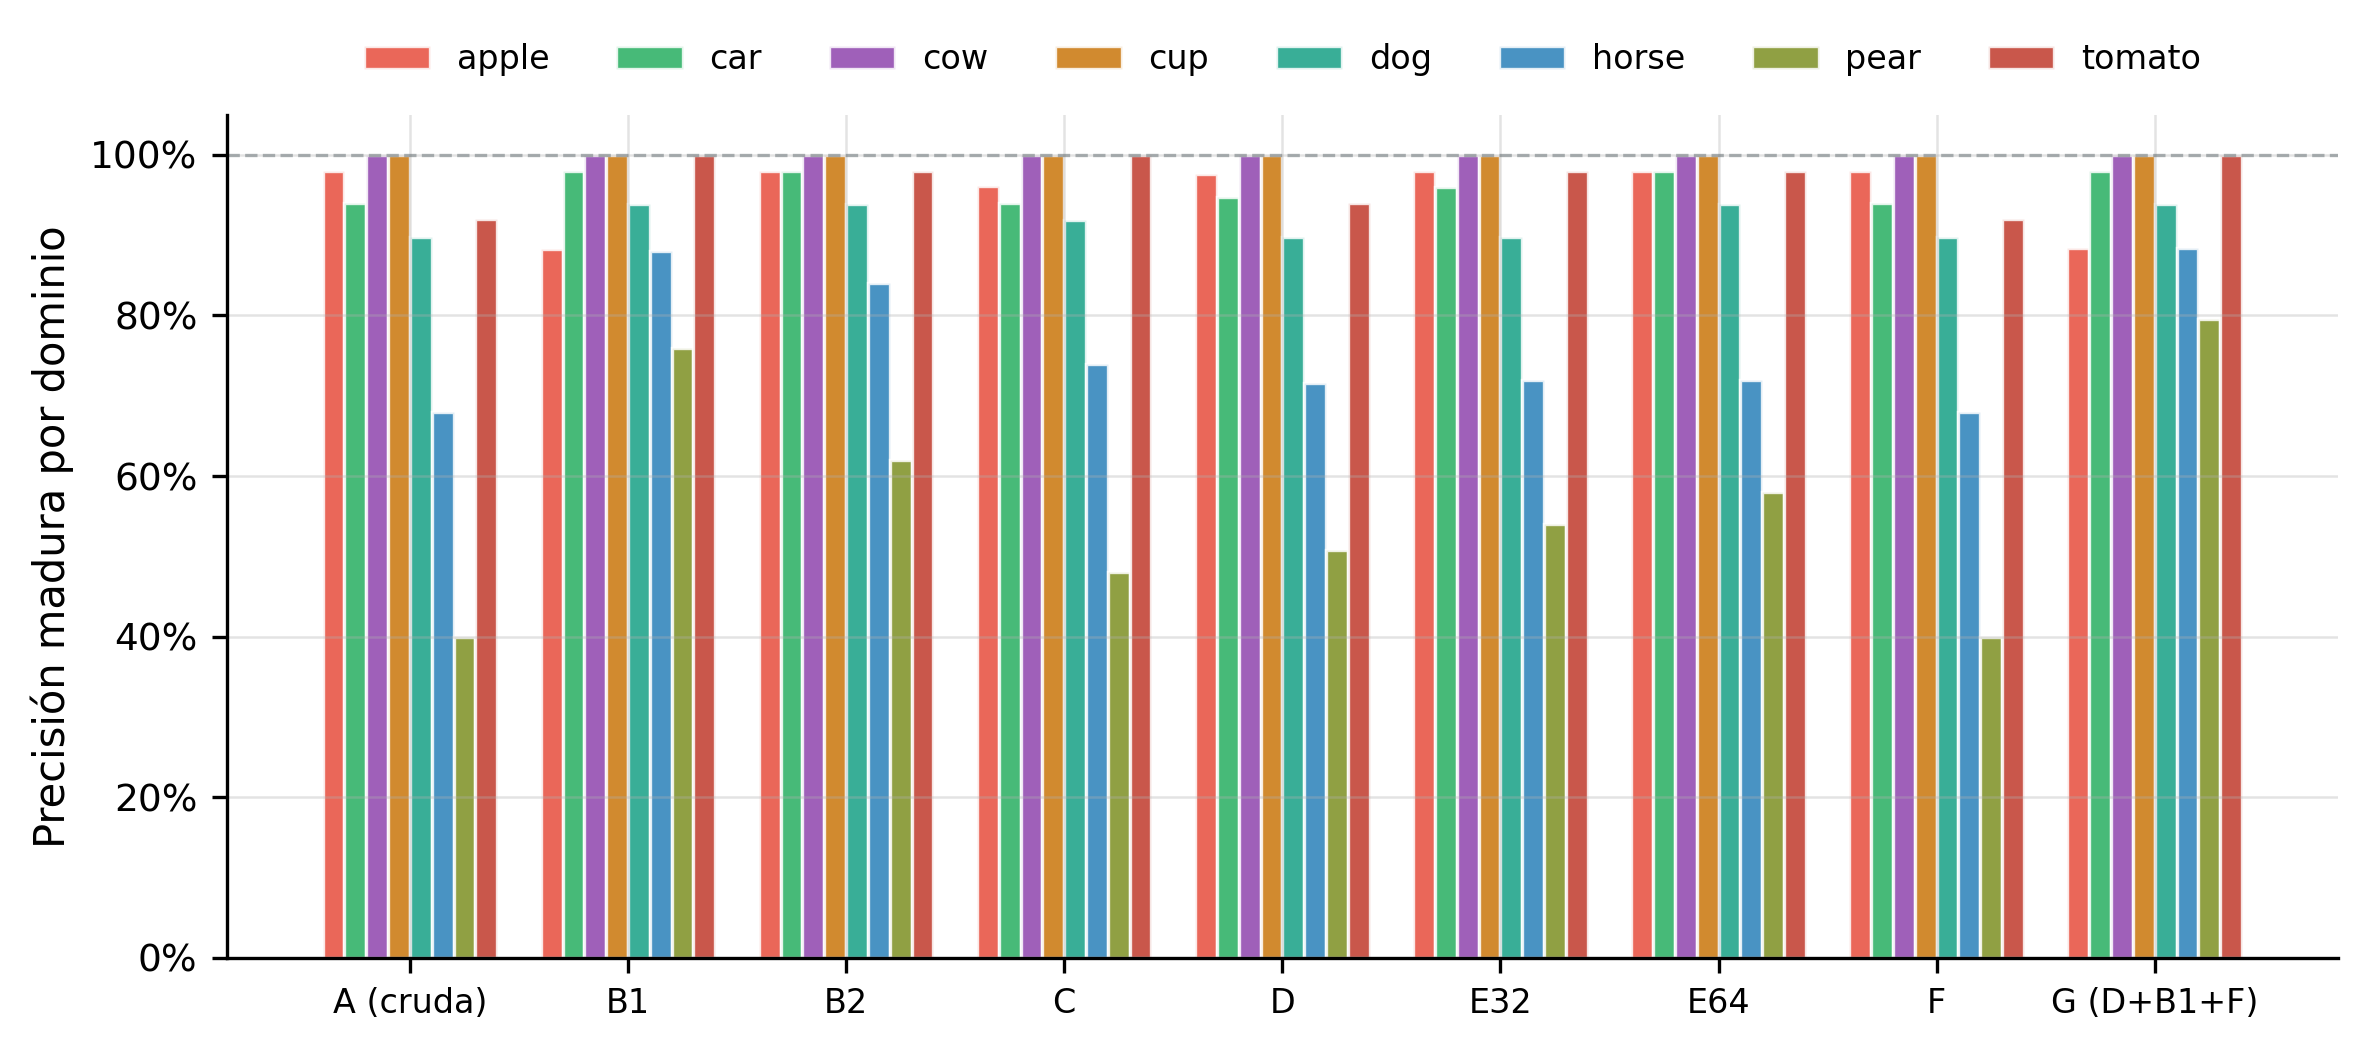
\includegraphics[width=\textwidth]{fig04_domain_accuracy_N400.png}
    \caption{Precisión madura por dominio y condición de la
    Tabla~\ref{tab:calibracion} ($N = 400$, media de 5 semillas).
    \texttt{pear} es el dominio más bajo en todas las condiciones; la lectura B1 lo lleva
    de 40 a 76\% respecto de la cruda (A), y a \texttt{horse} de 68 a 88\%.}
    \label{fig:dominio}
\end{figure}

\paragraph{Con B1, la participación de \texttt{apple} queda cerca del ideal.}
La Figura~\ref{fig:winner} muestra qué fracción de las victorias maduras se lleva cada
módulo.
Con la lectura cruda (A), \texttt{apple} se lleva el 20.5\%: es el sesgo de lectura que
B1 corrige.
Con B1 baja al 13.8\% (ideal 12.5\%), y el módulo que más se aleja del ideal es
\texttt{pear}, a 2.25 puntos (10.25\%).
La Sección~\ref{sec:disc-dominancia} analiza el origen del sesgo.

\begin{figure}[H]
    \centering
    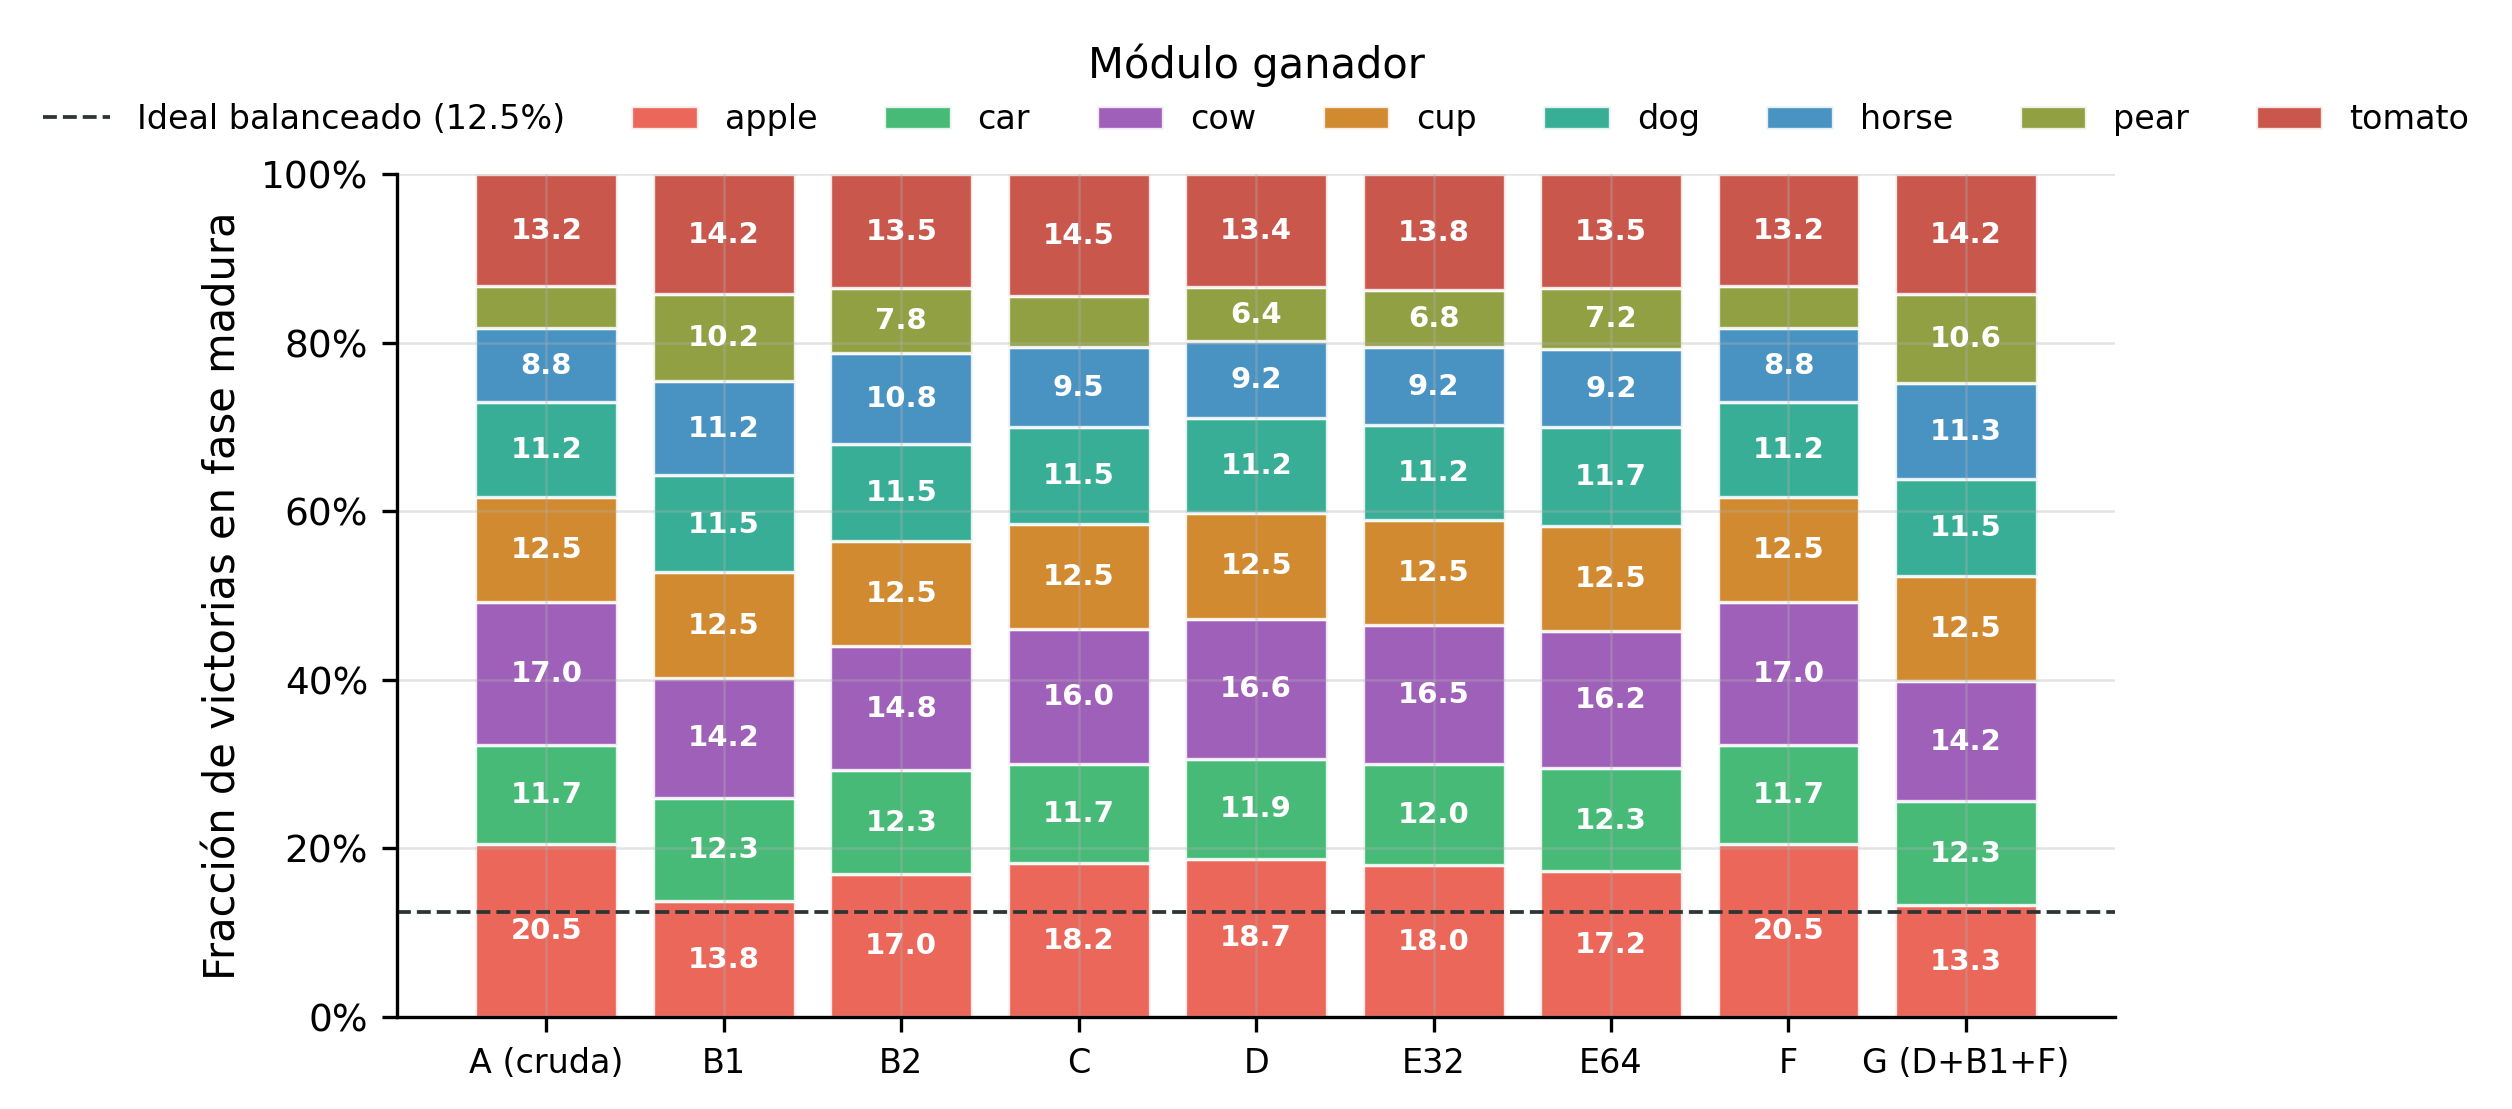
\includegraphics[width=\textwidth]{fig09_winner_distribution_N400.png}
    \caption{Distribución de módulos ganadores en fase madura por condición de la
    Tabla~\ref{tab:calibracion} ($N = 400$, media de 5 semillas; cifras en \%, sin cifra
    en los segmentos menores del 6\%).
    La línea discontinua marca el ideal balanceado de $1/8 = 12.5\%$, con el que se
    compara el segmento inferior (\texttt{apple}).}
    \label{fig:winner}
\end{figure}

\paragraph{Estado del directorio.}
La entropía del directorio transactivo es de 2.974 bits en la condición A y de 2.977 en
G, el 99.1\% del máximo ($\log_2 8 = 3$ bits): los conteos quedan casi parejos entre los
ocho módulos.
El sesgo que B1 corrige está en la lectura, no en los conteos
(Sección~\ref{sec:disc-b1}).

% ---------------------------------------------------------------
\subsection{Protocolo completo}
\label{sec:proto-completo}

El protocolo completo (fase temprana $\to$ formación del directorio $\to$ fase madura
con el TME apagado) se corrió sobre el subconjunto de 80 consultas (10 por clase).
Mide lo mismo que la calibración con el protocolo del sistema, pero el directorio se
forma con 10 consultas por dominio en lugar de unas 50; por eso su precisión madura es
menor que la del banco completo (Sección~\ref{sec:formacion}).

\paragraph{Fase temprana.}
El sistema alcanzó una precisión temprana del 81.2\% con una tasa de rechazo del 5.0\%;
los rechazos los decide la memoria, sin filtro de vocabulario
(Sección~\ref{sec:pipeline-semantico}).

\paragraph{Fase madura.}
Con la lectura B1, la precisión madura fue del 81.2\% y la fidelidad temprana-madura del
92.5\%; con la lectura cruda, la precisión madura baja al 72.5\%.
El directorio terminó con los conteos $[46, 16, 40, 25, 30, 18, 21, 31]$ para
(\texttt{apple}, \texttt{car}, \texttt{cow}, \texttt{cup}, \texttt{dog}, \texttt{horse},
\texttt{pear}, \texttt{tomato}) y una entropía de 2.914 bits sobre un máximo de 3.000.

\paragraph{Réplica con las 16 consultas de referencia.}
Con las 16 consultas de referencia del sistema (\texttt{TEST\_QUERIES}, 2 por dominio),
el enrutamiento acierta 15 de 16, con al menos un acierto en cada clase y conteos
$[12, 6, 6, 7, 5, 5, 4, 7]$;
el único error es una consulta de fruta con léxico compartido
(``a ripe green pear from the orchard'' $\to$ \texttt{apple}).

\paragraph{Sonda de rechazo fuera de dominio.}
Aparte del banco, se presentaron 12 consultas \emph{representables} (todas tienen vector
fastText) que describen objetos fuera de los ocho dominios.
La memoria rechazó 10 de 12 por contención (puntuación cero en los ocho módulos).
Las 2 restantes se enrutan porque comparten tokens con etiquetas legítimas de algún
dominio (p.\ ej.\ \textit{food}): la frontera entre ``fuera de dominio'' y ``comparte
conceptos con el dominio'' es semántica, no léxica.

% ---------------------------------------------------------------
\subsection[Parámetros nativos iota x kappa]{Parámetros nativos $\iota \times \kappa$}
\label{sec:param-iota-kappa}

Los dos parámetros propios de la EAM (Sección~\ref{sec:eam}) son la poda $\iota$, que
apaga durante la recuperación las celdas de peso menor que $\iota$ veces el peso medio
de las celdas no nulas, y el umbral relativo $\kappa$, que exige a la activación media
por celda de la proyección llegar a $\kappa$ veces la media de la memoria.
La pregunta es si alguno mejora la fase temprana o hace innecesaria la normalización B1.
Se barrió una cuadrícula con $\iota \in \{0, 0.25, 0.5, 1.0\}$ y siete valores de
$\kappa$: 0 y los cuantiles 10, 25, 50, 75, 90 y 100\,\% de esa razón, medida con
$\iota = 0$ sobre los 260 pares (token, módulo) del subconjunto de 80 consultas en que el
módulo contiene al token, lo que da
$\kappa \in \{0, 1.755, 1.801, 1.844, 1.937, 2.056, 2.107\}$.
La Tabla~\ref{tab:grid-iota-kappa} muestra la precisión temprana y el rechazo.

\begin{table}[H]
    \centering
    \caption{Precisión temprana y, entre paréntesis, tasa de rechazo (\%) en función de
    $\iota$ y $\kappa$ (80 consultas). Con $\iota \geq 0.25$ el valor no cambia con
    $\kappa$: la poda sube la razón que $\kappa$ compara por encima del mayor $\kappa$
    del barrido.}
    \label{tab:grid-iota-kappa}
    \small
    \begin{tabular}{cccccccc}
        \toprule
        & \multicolumn{7}{c}{$\kappa$} \\
        \cmidrule(lr){2-8}
        $\iota$ & 0 & 1.755 & 1.801 & 1.844 & 1.937 & 2.056 & 2.107 \\
        \midrule
        0.00 & 81.2 (5.0) & 77.5 (6.2) & 65.0 (10.0) & 57.5 (18.8) & 35.0 (45.0) & 18.8 (63.8) & 0.0 (100.0) \\
        0.25 & 82.5 (5.0)  & \multicolumn{6}{c}{igual en todas las columnas} \\
        0.50 & 75.0 (11.2) & \multicolumn{6}{c}{igual en todas las columnas} \\
        1.00 &  8.8 (86.2) & \multicolumn{6}{c}{igual en todas las columnas} \\
        \bottomrule
    \end{tabular}
\end{table}

\paragraph{Efecto de $\iota$.}
Una poda ligera ($\iota = 0.25$) quita algo de ruido de baja frecuencia: la fase
temprana pasa de 81.2 a 82.5\% y la madura con B1 de 81.2 a 83.8\% (la
Tabla~\ref{tab:grid-iota-kappa} solo da la fase temprana).
Una poda mayor destruye: $\iota = 0.5$ pierde 6 puntos con un rechazo del 11\%, y
$\iota = 1.0$ rechaza el 86\%.
La poda elimina conocimiento escaso pero válido antes de eliminar relaciones espurias.

\paragraph{Efecto de $\kappa$.}
Con $\iota = 0$, $\kappa$ solo rechaza: a medida que sube, la precisión baja de 81.2\%
a 0.0\% y el rechazo sube de 5.0\% a 100\%, y ninguna columna mejora la línea base.
El umbral relativo descarta por igual pistas válidas y espurias, porque la razón que
compara (entre 1.52 y 2.11) no separa a unas de otras.
Con $\iota \geq 0.25$, $\kappa$ no actúa en este rango: la poda concentra la activación
en las celdas que sobreviven y la media de la memoria no cambia, así que la razón
mínima sube a 2.33, 2.79 y 3.96, por encima del $\kappa$ máximo.
$\kappa$ no es una defensa contra el sesgo de masa.

\paragraph{Ninguna condición nativa sustituye a B1.}
En las dos condiciones nativas llevadas hasta la fase madura, la lectura cruda queda por
debajo de B1: 72.5\% frente a 81.2\% en la línea base y 80.0\% frente a 83.8\% en la
mejor condición nativa ($\iota = 0.25$, $\kappa = 0$).
También se probó dividir la puntuación temprana de cada módulo entre la media de su
memoria de contenido ($\div$\texttt{mem.mean}): \emph{empeora} la fase temprana (76.2\%)
y distorsiona los conteos del directorio, porque con el llenado por instancias las masas
de contenido ya están igualadas por construcción y esa corrección sobra.

% ---------------------------------------------------------------
\subsection{Formación del directorio transactivo}
\label{sec:formacion}

Se midió cuántas interacciones necesita el directorio para volverse utilizable y si
importa su orden: tras cada interacción $t$ de la fase temprana se evaluó la precisión
madura (lectura B1) sobre las 80 consultas, con el directorio tal como estaba en ese
momento, en cuatro condiciones: orden intercalado entre dominios, barajado (5 semillas),
bloqueado por dominio (todas las consultas de una clase y luego las de la siguiente) y
un control en orden intercalado que elige al ganador temprano con la puntuación cruda,
sin compuerta ni normalización.

\paragraph{Con 10 consultas por clase, ninguna condición llega al 90\%.}
Todas convergen al 81.2\% final.
Con ocho dominios y consultas que comparten léxico, 10 interacciones por dominio no
acumulan suficiente evidencia distintiva; el mismo protocolo con el banco completo
alcanza el 93.0\% (Sección~\ref{sec:calibracion}).

\paragraph{El orden afecta la velocidad, no el destino.}
Las cuatro condiciones terminan en el mismo estado: los conteos y la entropía de la
Sección~\ref{sec:proto-completo} (2.914 bits).
El orden sí cambia la velocidad: la precisión madura llega al 70\% tras 13 interacciones
en orden intercalado, tras 28 a 42 en orden barajado (según la semilla) y tras 59 en
orden bloqueado; al 75\%, tras 18, 40 a 51 y 71.
Esta invariancia del destino muestra que el directorio acumula evidencia conmutativa:
el orden solo determina cuándo se vuelve utilizable, no qué se aprende.

% ---------------------------------------------------------------
\subsection{Capacidad de llenado}
\label{sec:capacidad}

Se varió el número de imágenes registradas por clase,
$N \in \{25, 50, 100, 200, 328\}$, con el llenado imagen por imagen
(\textit{imagen--etiqueta}).
Una imagen se acepta si la memoria del módulo la contiene desde el lado de la imagen
(contención inversa, con $\xi = 0$); los \textit{falsos} se miden con imágenes de otras
clases presentadas al módulo.
La Tabla~\ref{tab:capacidad} resume las métricas.

\begin{table}[H]
    \centering
    \caption{Métricas de capacidad en función del número de imágenes registradas $N$
    por clase.
    ``Llenado propio'' y ``Prueba propia'': fracción de imágenes de la propia clase, de
    llenado y de prueba, que el módulo acepta; ``Falsos'': fracción de imágenes de otras
    clases que acepta.
    ``Enrutamiento'' es la precisión temprana sobre 80 consultas (reconocimiento por el
    contenido llenado con $N$ imágenes, sin directorio); ``Variedad $L_1$'' es la
    distancia media $L_1$ entre recuperaciones de una misma pista; $H$ es la entropía de
    la memoria de contenido.}
    \label{tab:capacidad}
    \small
    \setlength{\tabcolsep}{4pt}
    \begin{tabular}{ccccccc}
        \toprule
        $N$ & Llenado propio (\%) & Prueba propia (\%) & Falsos (\%) & Variedad $L_1$ & Enrutamiento (\%) & $H$ (bits) \\
        \midrule
         25  & 100 &  0 & 0 & 1.90 & 61.3 & 3.648 \\
         50  & 100 &  0 & 0 & 1.86 & 72.5 & 4.369 \\
        100  & 100 &  2 & 0 & 1.74 & 78.8 & 4.950 \\
        200  & 100 & 20 & 0 & 1.91 & 81.2 & 5.204 \\
        328  & 100 & 56 & 0 & 2.18 & 81.2 & 5.318 \\
        \bottomrule
    \end{tabular}
\end{table}

\paragraph{Generalización con el volumen de llenado.}
Con $\xi = 0$ el sistema no generaliza desde cero; la generalización a imágenes de prueba
aparece a medida que el llenado cubre más del espacio latente de la clase (del 0\% en
$N = 25$ al 56\% en $N = 328$), sin necesidad de ajustar $\xi > 0$ en el contenido.

\paragraph{Especificidad.}
Con el llenado de un latente por imagen, la tasa de falsos aceptados es del 0\% en todo
el rango de $N$ probado, con siete clases contrarias por módulo.

\paragraph{Enrutamiento y entropía.}
La precisión temprana crece con $N$ y se estabiliza en torno al 81\% desde $N = 200$; la
entropía de la memoria de contenido crece con $N$ y se satura (3.65, 4.37, 4.95, 5.20 y
5.32 bits), coherente con la acumulación de variedad.
El sistema opera con $N = 200$: ahí la precisión temprana ya se estabilizó, y quedan
\texttt{train[200:328]} para las interacciones visuales (Sección~\ref{sec:dataset}).

% ---------------------------------------------------------------
\subsection{Hemisferio visual}
\label{sec:hemisferio-visual}

El hemisferio visual opera en dos fases: formación (registro de percepciones reales de
\texttt{train[200:328]} en los directorios visuales) y evaluación (enrutamiento de las
656 imágenes de prueba mediante el directorio visual por módulo).

\paragraph{Fase A: formación con 1024 imágenes.}
Se presentaron 1024 imágenes (128 por clase) en orden intercalado.
Sobre las percepciones aceptadas, el enrutamiento visual acertó el 99.9\%, con un
rechazo del 0.8\% y una percepción rechazada antes de la memoria por el umbral de
energía.
Cada percepción aceptada registra sus 16 variantes; el registro completo del TME quedó
en $[2048, 2016, 2016, 2016, 2016, 2032, 2048, 2048]$, con entropía de 3.000 bits al
tercer decimal, el máximo con ocho módulos.
Los directorios visuales de cada módulo quedan entre 2.22 y 2.41 bits, con 2016--2048
registros propios contra 144--368 de cada otro módulo, como corresponde a un registro
perspectival.

\paragraph{Fase B: enrutamiento de imágenes de prueba.}
Las 656 imágenes de prueba se enrutaron mediante los directorios visuales por módulo
($M^R_{\mathrm{dir}}$) con lectura B1 estricta ($\xi = 0$, directorios perspectivales):
cada imagen entra por un módulo no especialista, que la redirige o la rechaza.
El resultado fue de 631 de 656 imágenes (96.2\%) asignadas correctamente, 23 rechazadas
(3.5\%; cuatro de ellas antes de la memoria, por el umbral de energía) y dos falsos
enrutamientos (0.3\%); sobre las aceptadas, la precisión es del 99.7\%.

\paragraph{Más variantes, más cobertura.}
El directorio visual no tolera huecos ($\xi = 0$; la razón está en la
Sección~\ref{sec:operaciones}): con $\xi = 2$, el enrutamiento del dominio propio baja a
medida que el módulo presencia más dominios ajenos (experimento 10).
La palanca para la cobertura es densificar el llenado, no tolerar huecos.
El experimento 13 lo mide sobre las 656 imágenes de prueba: registrar en el directorio 16
variantes por percepción, en lugar de una, lleva su aceptación del 73.6 al 96.2\,\% (con
4 variantes, 87.7\,\%); con 16 variantes también en el contenido, la \emph{cobertura de
punta a punta} (imágenes enrutadas a su clase cuyo destino además responde) pasa de 66.5
a 94.5\,\%, y el rechazo de la fase A baja del 4.2 al 0.8\,\%.
En ese experimento, con una o 4 variantes en el directorio no hay enrutamientos falsos y
con 16 hay uno; el sistema, con sus 16 variantes, enruta mal dos de las 656 imágenes
(Sección~\ref{sec:limitaciones}).

\paragraph{Evocación de dominio: imagen $\to$ palabras.}
Sobre las primeras 15 imágenes de prueba de cada clase que el enrutamiento acepta (116 de
120), la evocación inversa desde el módulo destino (recuperación $\beta$ desde el
latente, decodificada por similitud coseno top-3) produjo al menos una etiqueta del
vocabulario de la clase real en 113 de 116 (97.4\%) de los casos.

\paragraph{El rechazo y la salida semántica los decide la memoria.}
Reconocimiento, rechazo y reconstrucción son operaciones de la propia memoria: el
codificador ResNet18 solo convierte la imagen en una pista latente, y a partir de ahí la
EAM decide.
La Figura~\ref{fig:rechazo-imagenes} ilustra el rechazo: imágenes reales que la memoria
contiene se aceptan, mientras que imágenes reales no contenidas y las sondas sintéticas
de ruido y de píxeles barajados reciben puntuación cero en los ocho módulos y se
rechazan, sin que intervenga ningún filtro externo.
La tercera sonda, un lienzo gris uniforme, no llega a la memoria: la norma de su
latente (10.7) queda por debajo del umbral de energía $\tau = 16.61$
(Sección~\ref{sec:percepcion}), igual que una vista real de \texttt{cow} del panel.
Sin ese umbral, el contenido sí le daría soporte. El experimento 14 localizó la causa:
el codificador lleva las entradas sin estructura (gris uniforme, un objeto desenfocado o sin
contraste) a latentes de norma baja que caen dentro de la envolvente por coordenada de
los animales. Los grises de nivel 120 a 160 (el del panel, 127, cae en ese tramo) los
aceptan a la vez \texttt{cow}, \texttt{dog} y \texttt{horse}, aunque la instancia real
más cercana está a entre 2.4 y 2.9 veces la mediana de la distancia intraclase.
No es cualquier fondo liso: de 12 sólidos de color se aceptan 2.
Esos grises tienen norma de 10.7 a 13.0, y el umbral los rechaza.
Las entradas degeneradas que sí pasan el umbral se discuten en la
Sección~\ref{sec:limitaciones}.
La Figura~\ref{fig:imagen-etiquetas} muestra la salida semántica: para cada imagen
aceptada, la reconstrucción es lo que la memoria \emph{evoca} (decodificación de la
recuperación desde la lectura latente $M^R$), no la imagen de entrada, y el sistema devuelve
las etiquetas asociadas.
Que la reconstrucción difiera de la entrada es esperado y honesto: refleja que decide
la distribución acumulada en la memoria.

\begin{figure}[H]
    \centering
    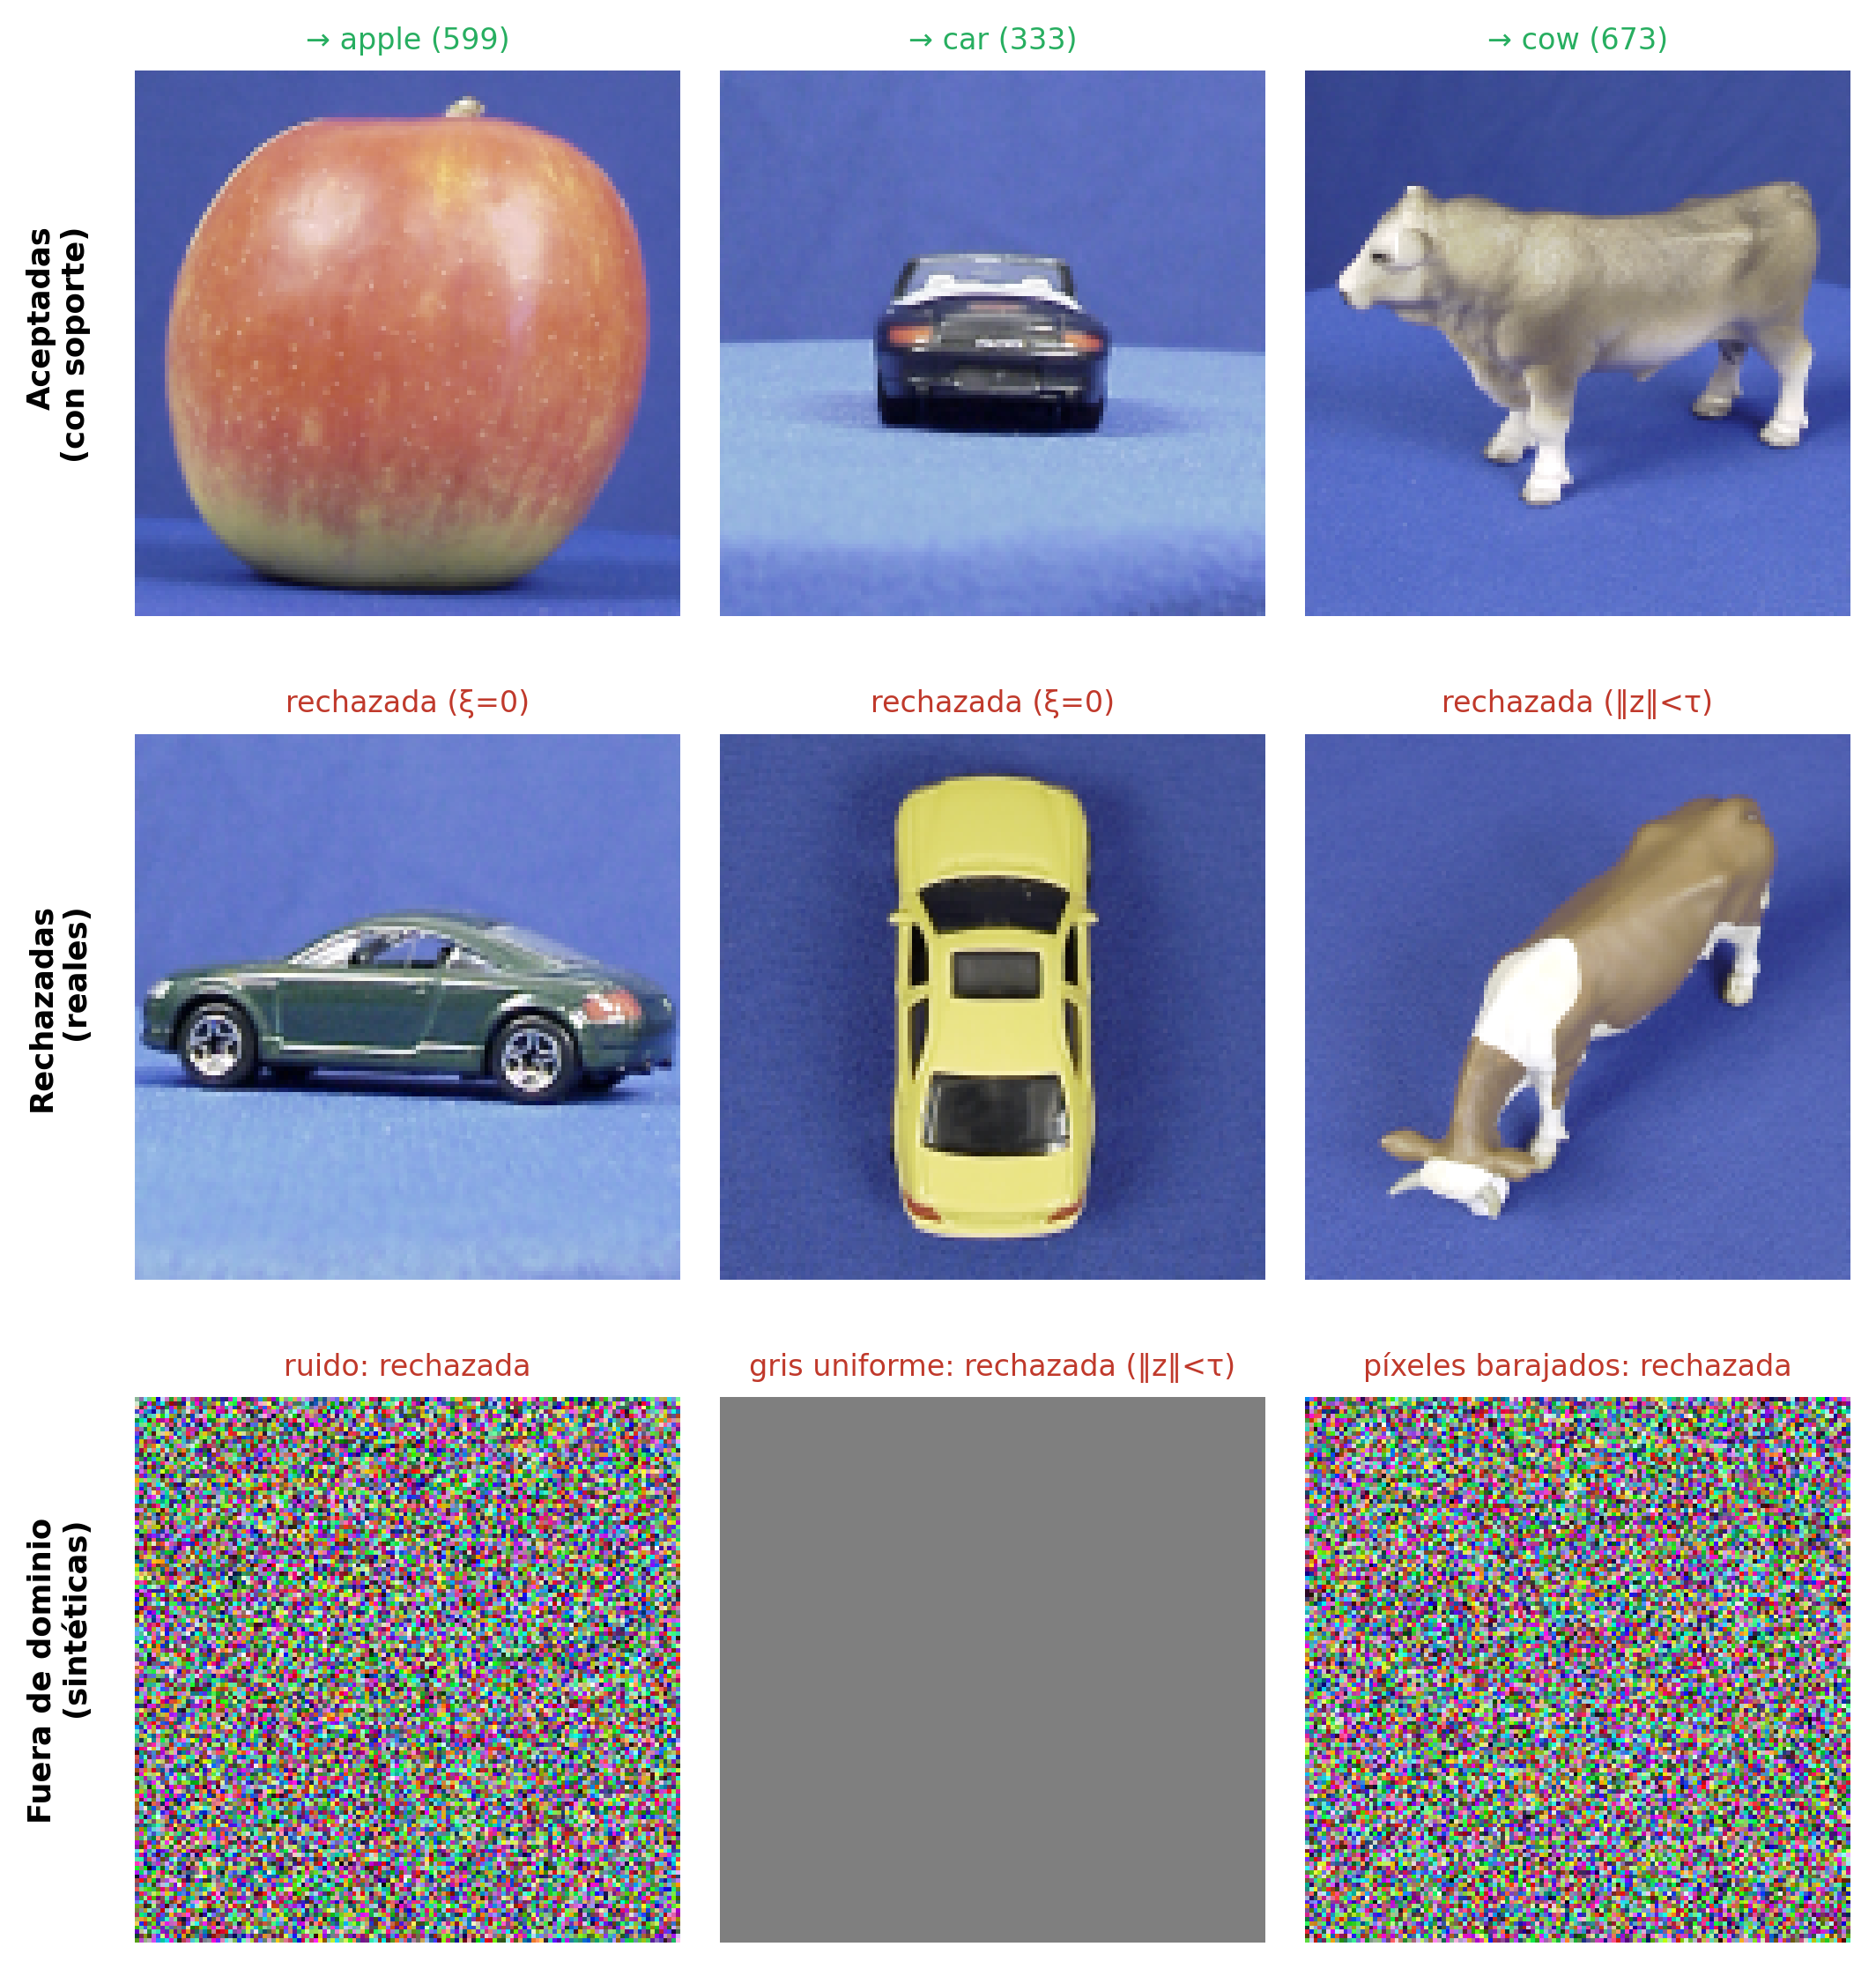
\includegraphics[width=0.85\textwidth]{fig15_image_rejection.png}
    \caption{Rechazo de imágenes en el hemisferio visual (sin filtro léxico), con el umbral
    de energía $\tau$ y la contención en el mismo orden que el sistema. Arriba: imágenes de
    prueba aceptadas por el contenido, con el módulo de mayor soporte y su puntuación de
    contención. En medio: imágenes de prueba rechazadas, dos porque ningún módulo las
    contiene ($\xi = 0$) y una vista de \texttt{cow} porque la norma de su latente no
    alcanza $\tau$. Abajo: sondas sintéticas; el ruido y los píxeles barajados reciben
    puntuación cero en los ocho módulos, y el gris uniforme se rechaza antes de la memoria
    por el umbral $\tau$.}
    \label{fig:rechazo-imagenes}
\end{figure}

\begin{figure}[p]
    \centering
    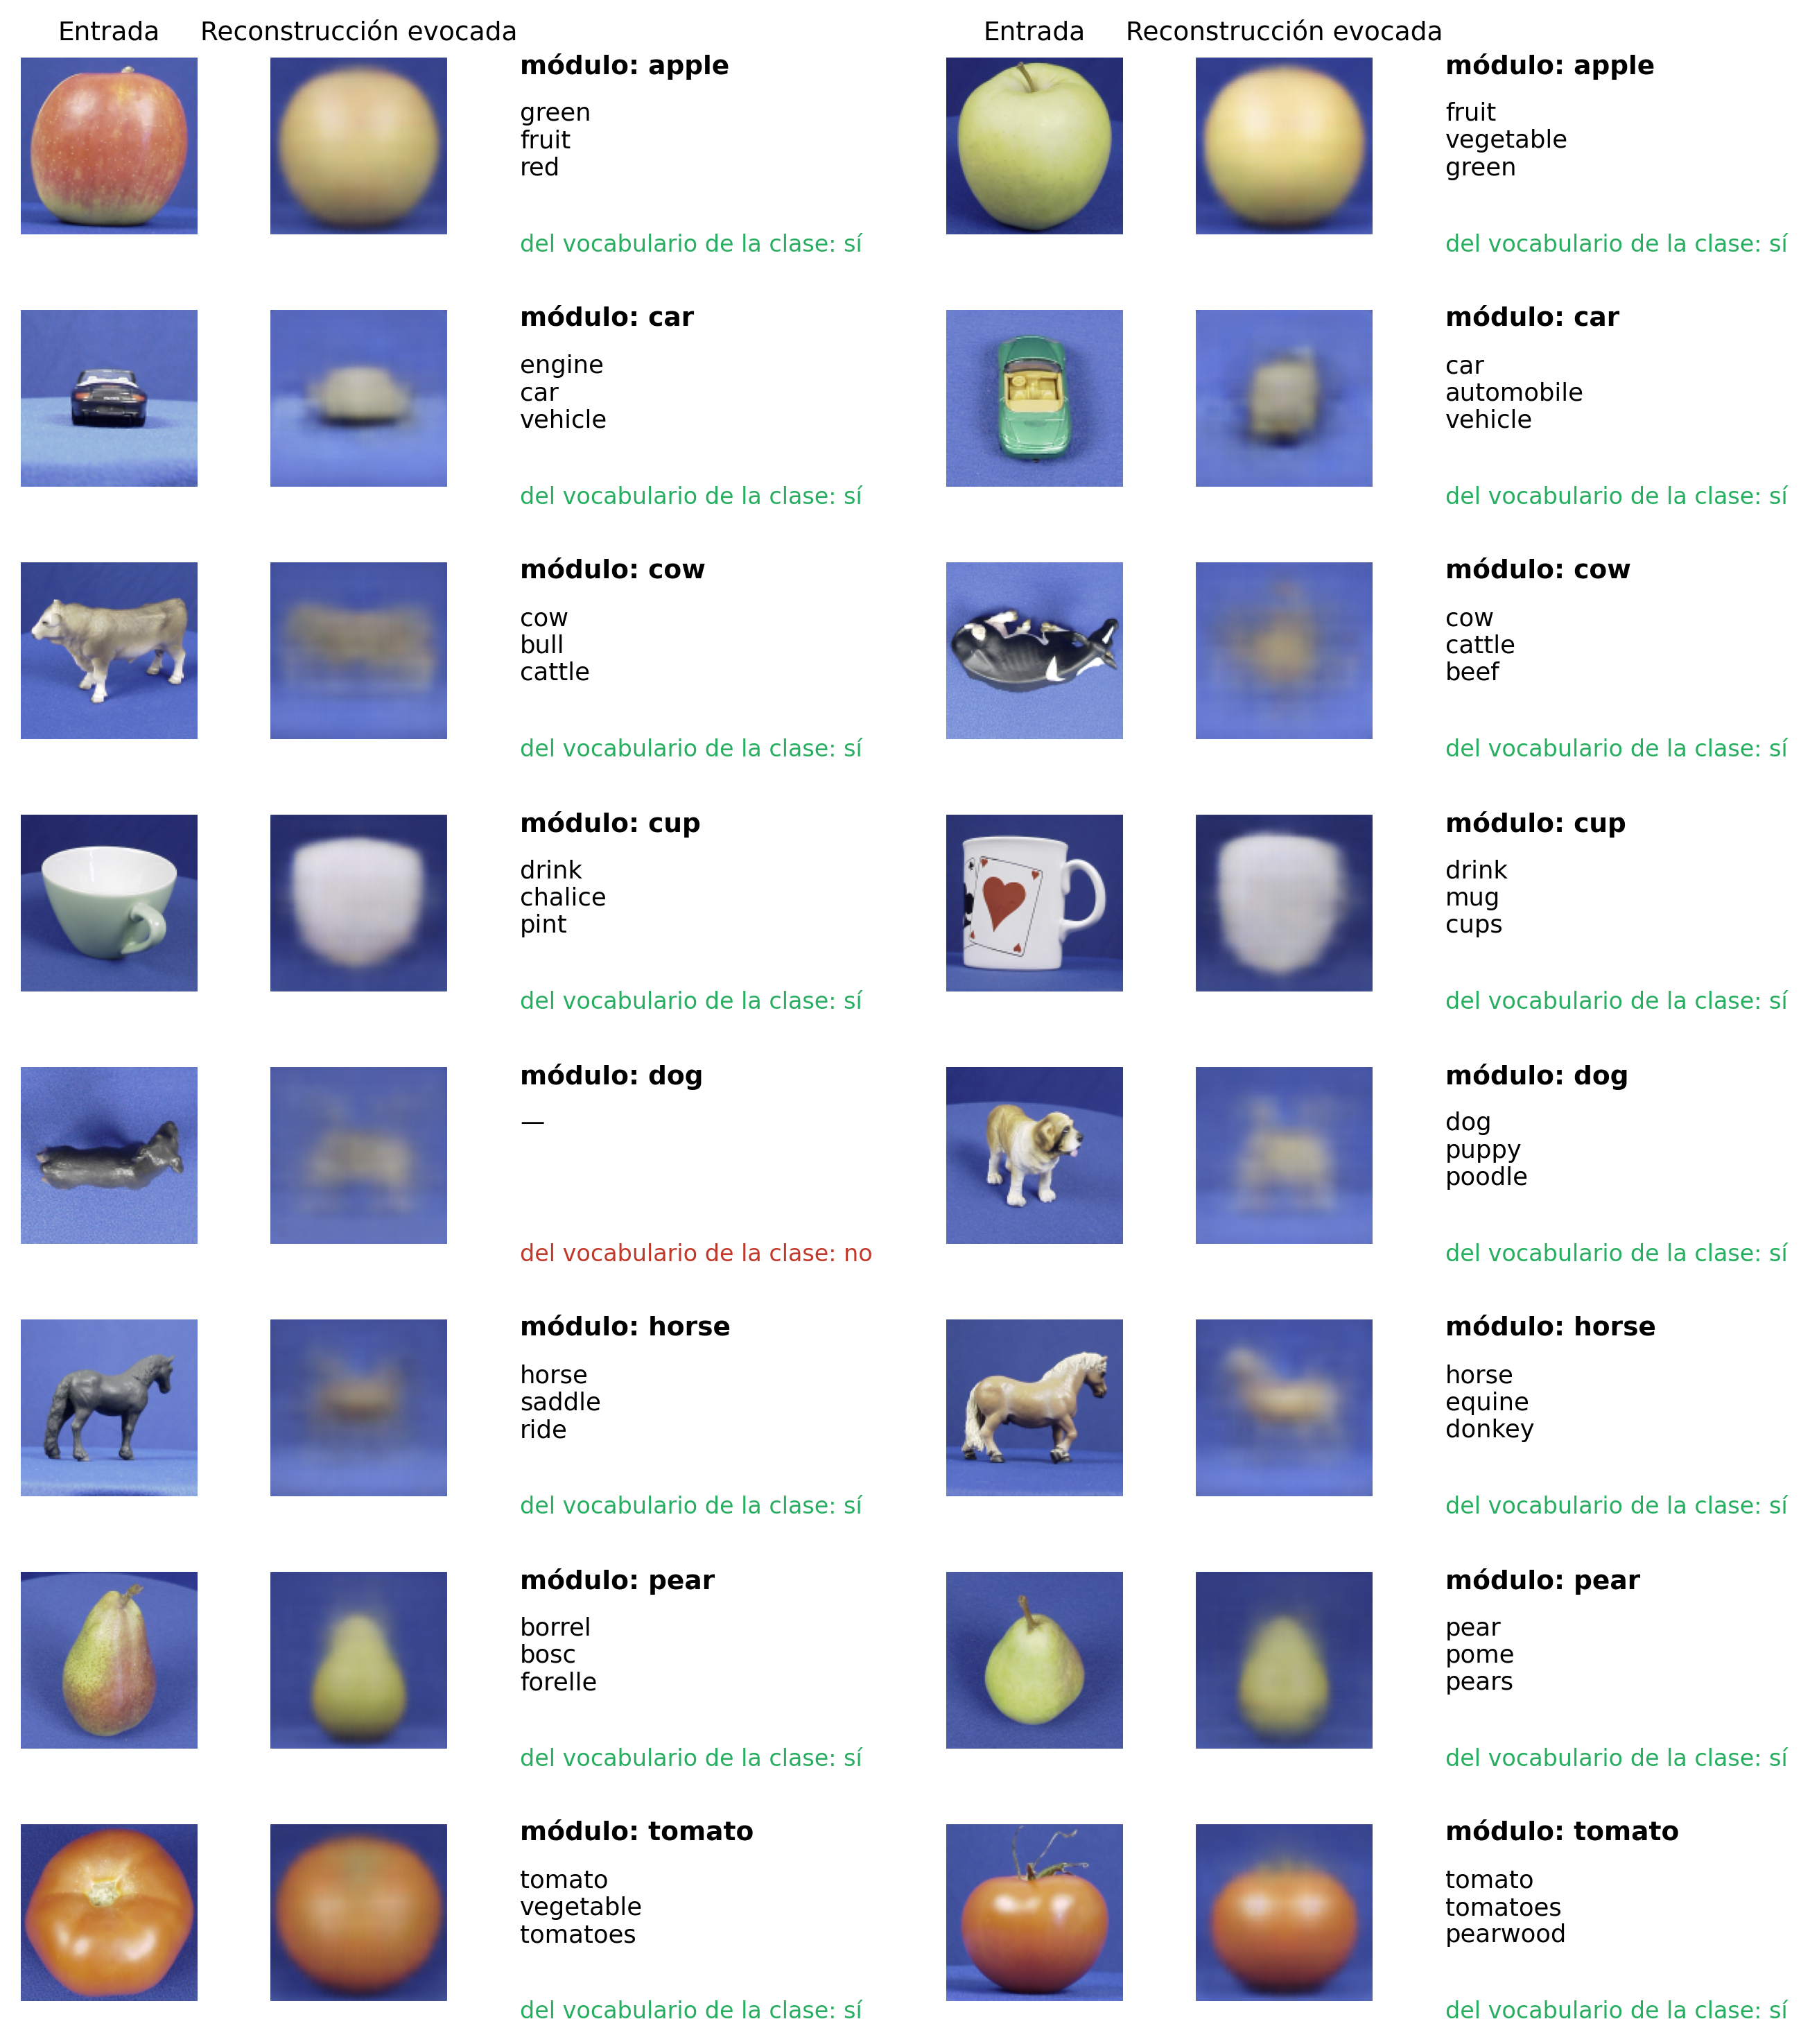
\includegraphics[width=\textwidth]{fig16_image_to_labels.png}
    \caption{Salida semántica imagen $\to$ etiquetas: las dos primeras imágenes de prueba
    de cada clase que pasan el umbral de energía y que algún módulo contiene (el de mayor
    soporte, sin pasar por el directorio).
    Por imagen: la entrada, la reconstrucción que evoca la memoria (no la entrada) y las
    tres etiquetas recuperadas, con la marca de si alguna es del vocabulario de la clase
    real.
    En 15 de los 16 ejemplos alguna etiqueta es del dominio; en el restante
    (\texttt{dog}) la recuperación no devuelve etiquetas.
    Con el directorio, sobre las primeras 15 imágenes de prueba de cada clase que el
    enrutamiento acepta (116), la evocación acierta el 97.4\% (113).}
    \label{fig:imagen-etiquetas}
\end{figure}

% ---------------------------------------------------------------
\subsection{Generalización a objetos nuevos}
\label{sec:objetos-nuevos}

La partición principal separa imágenes, no objetos: los diez objetos de cada clase
aportan vistas al llenado y a la prueba (Sección~\ref{sec:dataset}), así que las cifras
anteriores miden vistas nuevas de objetos conocidos.
La generalización a objetos nuevos se midió aparte (experimento 16), con una validación
\textit{leave-one-object-out} de diez pliegues: en cada pliegue, el contenido y la fase A
se construyen con nueve objetos por clase, y sobre los mismos modelos se evalúan las 41
vistas del objeto reservado de cada clase y 41 vistas no usadas de los objetos que sí
contribuyeron.
La cobertura de punta a punta es del 89.2\,\% [85.1, 93.2] con objetos nuevos y del
95.5\,\% [95.1, 95.9] con objetos conocidos; la brecha es de 6.3 puntos [2.5, 10.4]
(intervalos de 95\,\% por remuestreo de los pliegues).
El enrutamiento correcto sobre las imágenes aceptadas es del 99.9\,\% en los dos bancos,
y los falsos enrutamientos con objetos nuevos son 2 de 3280 (un \texttt{cow} y un
\texttt{horse}, enviados a \texttt{dog}): la envolvente por coordenada cubre a un objeto
que no contribuyó a ella, y cuando no lo cubre lo rechaza.
La brecha no se reparte entre clases sino que se concentra en objetos concretos: 71 de
los 80 objetos reservados superan el 70\,\%, y nueve (dos manzanas, dos peras, dos
perros, una taza, un coche y una vaca) concentran el 57\,\% de los fallos.

% ---------------------------------------------------------------
\subsection{Línea base: una sola EHAM con las ocho clases}
\label{sec:eham-unica}

Esta sección mide qué aporta repartir el contenido entre ocho especialistas frente a
guardarlo todo en una sola memoria.
Se construyó una EHAM única con los mismos pares etiqueta--latente que reciben los ocho
especialistas (25\,600 con 200 imágenes por clase y 16 variantes) y se evaluó con las
mismas operaciones de reconocimiento con compuerta y de recuerdo desde la etiqueta
(\texttt{recognize\_gated}, \texttt{recall\_from\_left}), sin enrutamiento.
Se compararon tres brazos: la \emph{EHAM única}; los especialistas con el módulo elegido
por la verdad de terreno (\emph{oráculo}, un techo), y el \emph{protocolo} transactivo
completo, que elige el módulo con el directorio.
Las consultas de texto son las 171 del banco que no se usaron para formar los
directorios (las otras 240 los forman); las de imagen, las primeras 10 imágenes de
prueba de cada clase.
Se corrieron 10 semillas con 25, 50, 100 y 200 imágenes por clase.
Cada recuerdo se juzga por la clase de la instancia real más cercana (juez 1-NN) y por
la distancia a ella.
Con 200 imágenes por clase, cuatro de los ocho especialistas reconstruidos son idénticos
bit a bit a las memorias del sistema; los otros cuatro difieren porque el experimento
recalcula los latentes en GPU, y el redondeo puede mover un registro al nivel vecino.
La Tabla~\ref{tab:eham-unica} resume los resultados; las tablas completas, con sus
intervalos, están en \texttt{results/experimento11/}.

\begin{table}[H]
    \centering
    \caption{Una sola EHAM contra los especialistas, por número de imágenes de llenado
    por clase (media de 10 semillas). Texto: 171 consultas reservadas; clase correcta
    según el juez 1-NN, distancia a la instancia real más cercana y, en el protocolo,
    enrutamiento a la clase de la consulta. Imagen $\to$ texto: 80 imágenes de prueba;
    fracción respondida y fracción respondida con el dominio de otra clase. Fuera de
    dominio: consultas aceptadas de 40; entre paréntesis, con la doble compuerta de
    contenido.}
    \label{tab:eham-unica}
    \small
    \begin{tabular}{llcccc}
        \toprule
        & & \multicolumn{4}{c}{Imágenes por clase} \\
        \cmidrule(lr){3-6}
        Medida & Brazo & 25 & 50 & 100 & 200 \\
        \midrule
        Clase correcta (\%)        & EHAM única & 97.6 & 97.5 & 97.6 & 96.9 \\
                                   & Protocolo  & 96.9 & 98.8 & 98.8 & 98.3 \\
                                   & Oráculo    & 100  & 100  & 100  & 100  \\
        \midrule
        Enrutamiento correcto (\%) & Protocolo  & 95.3 & 97.4 & 97.4 & 97.0 \\
        \midrule
        Distancia a la instancia   & EHAM única & 22.9 & 26.6 & 29.4 & 32.5 \\
        real más cercana           & Protocolo  & 19.0 & 20.7 & 23.8 & 27.0 \\
                                   & Oráculo    & 18.2 & 20.4 & 23.3 & 26.8 \\
        \midrule
        Imagen $\to$ texto:        & EHAM única & 78.7 & 95.0 & 98.8 & 100  \\
        responde (\%)              & Oráculo    & 43.8 & 75.0 & 92.5 & 97.5 \\
                                   & Protocolo  & 41.2 & 67.5 & 78.7 & 81.2 \\
        \midrule
        Imagen $\to$ texto:        & EHAM única & 5.5  & 7.5  & 10.5 & 10.9 \\
        dominio ajeno (\%)         & Oráculo    & 0.1  & 1.9  & 2.6  & 4.1  \\
                                   & Protocolo  & 0.2  & 1.8  & 2.2  & 3.0  \\
        \midrule
        Fuera de dominio           & EHAM única & 2     & 2     & 5     & 8     \\
        aceptadas (de 40)          & Protocolo  & 4 (2) & 4 (2) & 4 (2) & 4 (2) \\
                                   & Oráculo    & 2     & 2     & 2     & 2     \\
        \bottomrule
    \end{tabular}
\end{table}

\paragraph{Acierto de clase.}
Con 25 imágenes por clase la EHAM única acierta la clase algo más que el protocolo
(97.6\,\% frente a 96.9\,\%), con intervalos de 95\,\% que se solapan ($[97.4, 97.8]$ y
$[96.3, 97.6]$).
Desde 50 el orden se invierte y los intervalos se separan (con 200, $[97.9, 98.6]$ para
el protocolo y $[96.7, 97.1]$ para la EHAM única).
Lo que cuesta elegir el módulo con el directorio en lugar de con la verdad de terreno, la
distancia del protocolo al oráculo, es de 3.1 puntos con 25 imágenes por clase y de 1.2
a 1.7 desde 50.

\paragraph{Fidelidad del recuerdo.}
La respuesta de la EHAM única queda más lejos de la instancia real más cercana en los
cuatro cortes, pero su brecha con el oráculo no crece con el contenido: 4.6, 6.2, 6.1 y
5.7 (calculada antes de redondear).
Cuando la primera pista reconocida es una etiqueta compartida entre clases
(\emph{fruit}, \emph{animal}, \emph{red}; el 3.5\,\% de las respuestas), la EHAM única
acierta la clase entre el 48 y el 52\,\%, y ninguna clase por sí sola sostiene más del
74--77\,\% de las coordenadas de su patrón; el protocolo acierta entre el 79 y el
84\,\%, y el oráculo el 100\,\%.

\paragraph{Imagen $\to$ texto.}
La EHAM única responde más imágenes y se equivoca más de dominio: con 200 imágenes por
clase responde a todas, pero el 10.9\,\% con un dominio ajeno, frente al 4.1\,\% del
especialista elegido por el oráculo y el 3.0\,\% del protocolo, que en este experimento
forma su directorio visual sin variantes.

\paragraph{Fuera de dominio.}
La EHAM única acepta más consultas fuera de dominio a medida que crece el contenido; el
oráculo acepta 2 de 40 en todos los cortes, y el protocolo 4, que la doble compuerta de
contenido (el módulo destino debe contener la pista) baja a 2.

\subsection{Una memoria de contenido por módulo}
\label{sec:una-memoria}

Cada módulo guarda su contenido en una sola memoria heteroasociativa (en adelante, la
hetero), y las lecturas homoasociativas que usa se calculan de ella
(ecuación~\eqref{eq:marginal}).
Esta sección la compara con la arquitectura que guarda, junto a la hetero de cada
módulo, dos memorias homoasociativas llenadas aparte (las homo), una por dominio, como
fuente de pesos.
Con el llenado imagen--etiqueta, la homo latente recibe los mismos registros que el lado
latente de la hetero, y su relación es idéntica, celda por celda en los ocho módulos, a
la lectura $M^{R}$.
La homo de etiquetas registra cada palabra una vez por su frecuencia y no una vez por
imagen: tiene el mismo soporte que $M^{L}$, con conteos multiplicados por un
factor de 21 a 95 que varía entre celdas.

Se volvió a correr la batería completa con una sola memoria de contenido por módulo,
leyendo los pesos de la hetero.
En imagen, contención, rechazo, enrutamiento y evocación dan las mismas decisiones
imagen por imagen (631 de 656 en el enrutamiento de prueba, 113 de 116 en la evocación).
En texto cambian los recuerdos muestreados, tanto como al cambiar la semilla, y una
parte pequeña de las decisiones donde pesan las lecturas de etiquetas: el 1.3\,\% de
los destinos del protocolo en la comparación con una sola EHAM
(Sección~\ref{sec:eham-unica}), una consulta de 80 en la curva de capacidad con 50
imágenes por clase, y las columnas con $\kappa > 0$ del barrido, cuyos cuantiles se
recalculan sobre la lectura.
Todas las cifras de este documento son las de una sola memoria de contenido.

Para buscar algo que las memorias homo hicieran y la hetero no, se compararon las dos
arquitecturas con los mismos datos: 100 de las 200 imágenes de llenado de cada módulo
con su palabra y las otras 100 sin ella.
En la arquitectura con homo, la homo latente recibe todas y la hetero solo las
emparejadas; con una sola memoria, las imágenes sin palabra se registran en el borde de
valor indefinido. Por cada imagen se leen dos cosas: si el módulo la \emph{nombra} (la
proyección imagen$\to$texto no deja columnas vacías) y si le es \emph{familiar} (la homo
o la lectura latente la contienen).
Con las memorias intactas, las dos responden lo mismo consulta por consulta (2252
consultas): de las 800 imágenes sin palabra, la hetero nombra 722 por su parecido con
las emparejadas y 78 quedan reconocidas sin nombre.
Ninguna de las dos recupera una imagen concreta a partir de la mitad de sus
coordenadas: lo completado queda tan cerca de la original como de otra imagen del mismo
módulo (2.23 y 2.24 niveles de 32), porque cada coordenada se sortea de su propia
columna.

La Tabla~\ref{tab:lesion} muestra qué pasa al destruir al azar una fracción $f$ de las
celdas de la hetero.
Nombrar se lee de la proyección imagen$\to$texto (el recuerdo se reconoce si y solo si
ninguna columna queda vacía) y cae igual en todas las condiciones.
Con una memoria homo aparte e intacta, la familiaridad no cambia.
Con una sola memoria y el daño al azar, la familiaridad leída de la hetero tampoco cae
mientras queda algo que nombrar: entre el 5 y el 25\,\% de celdas destruidas el módulo
ya no nombra ninguna imagen y reconoce 795 a 800 de 800.
Una cuarta condición, que no está en la tabla, pasa el conteo de cada celda dañada al
borde en lugar de borrarlo, y conserva la familiaridad de las 800 imágenes en todo el
rango.
Si el mismo daño alcanza también a la homo, la familiaridad es lo primero que se
pierde: una celda de la homo es un punto único, mientras que una celda de la lectura
suma las de los 17 valores de etiqueta (los 16 niveles y el indefinido).
Ninguna lectura de la arquitectura con homo queda fuera del alcance de una sola memoria
por módulo.

\begin{table}[H]
\centering
\caption{Lesión de la memoria de contenido sobre las 800 imágenes emparejadas
(100 por módulo). $f$: fracción de celdas de la hetero destruidas al azar.
\emph{Nombra}: la proyección imagen$\to$texto no deja columnas vacías; es igual en las
tres condiciones. \emph{Familiar}: la homo o la lectura latente contiene la imagen.
Homo intacta: memoria homo aparte, sin daño. Una memoria: la lectura de la hetero
dañada. Homo dañada: la homo pierde además la misma fracción de sus celdas.}
\label{tab:lesion}
\small
\begin{tabular}{ccccc}
\toprule
$f$ & Nombra & Familiar, homo intacta & Familiar, una memoria & Familiar, homo dañada \\
\midrule
0    & 800 & 800 & 800 & 800 \\
0.01 &  64 & 800 & 800 & 416 \\
0.05 &   0 & 800 & 800 &  32 \\
0.25 &   0 & 800 & 795 &   0 \\
0.5  &   0 & 800 & 675 &   0 \\
0.75 &   0 & 800 &  15 &   0 \\
\bottomrule
\end{tabular}
\end{table}

\subsection{Costo computacional}
\label{sec:costo}

Se midió el tiempo de pared (\textit{wall-clock}) de reproducir el sistema completo
desde cero, de la partición del conjunto de datos a la fase madura, en una laptop con
un Intel Core Ultra 7 265HX (20 hilos lógicos) y 16.6~GB de RAM, con la GPU oculta:
todo corre en CPU.
La Tabla~\ref{tab:costo} resume los tiempos.

\begin{table}[H]
    \centering
    \caption{Costo computacional de reproducir el sistema desde cero (etapas 1 a 8,
    solo CPU). Fuente: \texttt{results/computational\_cost/nov2026\_cpu/}.}
    \label{tab:costo}
    \small
    \begin{tabular}{lr}
        \toprule
        Componente & Tiempo \\
        \midrule
        Entrenamiento del codificador ResNet18 (50 épocas, 2624 imágenes) & 21.5 min \\
        Vocabulario: ConceptNet y fastText & 0.6 min \\
        Llenado de las memorias de contenido (8 módulos, 3200 registros cada uno) & 37.4 min \\
        Fases temprana y madura de texto & 3.4 min \\
        Hemisferio visual (fase A con 1024 imágenes, fase B con 656, evocación) & 40.0 min \\
        \midrule
        Sistema completo (etapas 1--8) & \textbf{102.9 min} \\
        \bottomrule
    \end{tabular}
\end{table}

El sistema completo se reproduce en 102.9 minutos.
La parte más cara no es el entrenamiento del codificador, la única con gradientes y
retropropagación (21.5 min), sino las memorias: el llenado de las ocho memorias de
contenido y el hemisferio visual suman 77.4 minutos, tres cuartas partes del total.
Ninguna de las dos entrena nada: registran vectores cuantizados en las memorias
(200 imágenes por 16 variantes en cada módulo) y los leen para decidir.
Las fases de texto, con el banco de 411 consultas, tardan menos de cuatro minutos.

\section{Discusión}
\label{sec:discusion}

% ---------------------------------------------------------------
\subsection{La maquinaria transactiva funciona con ocho dominios; la representación es el límite}
\label{sec:disc-escala}

El resultado central separa dos responsabilidades: la maquinaria transactiva funciona
con ocho dominios, y los límites aparecen en la \emph{representación}.
Los componentes de la maquinaria (los directorios heteroasociativos, la lectura B1, el
rechazo por contención, la actualización perspectival del directorio (en imagen) y la
coordinación punto a punto) funcionan sin ajustes por dominio.
En imagen, el registro completo de percepciones de la fase A queda balanceado
(3.000 bits, el máximo con ocho módulos), y los directorios visuales de los módulos
enrutan las imágenes de prueba con dos falsos enrutamientos en 656
(Sección~\ref{sec:hemisferio-visual}).
En texto, las pistas se cuantizan por magnitud sobre una escala global
(Sección~\ref{sec:pipeline-semantico}), que puebla los 16 niveles del alfabeto (una
binarización por signo usaría 2), y con esa representación la precisión temprana sobre
el banco de 411 consultas es del 90.0\%.
Lo que la representación no quita es el solapamiento entre dominios: la
Figura~\ref{fig:espacio-semantico} muestra que persiste, porque es propiedad del léxico
(tres frutas, tres animales), y en él cae la mayoría de los errores que quedan
(Sección~\ref{sec:disc-dominancia}).

\begin{figure}[H]
    \centering
    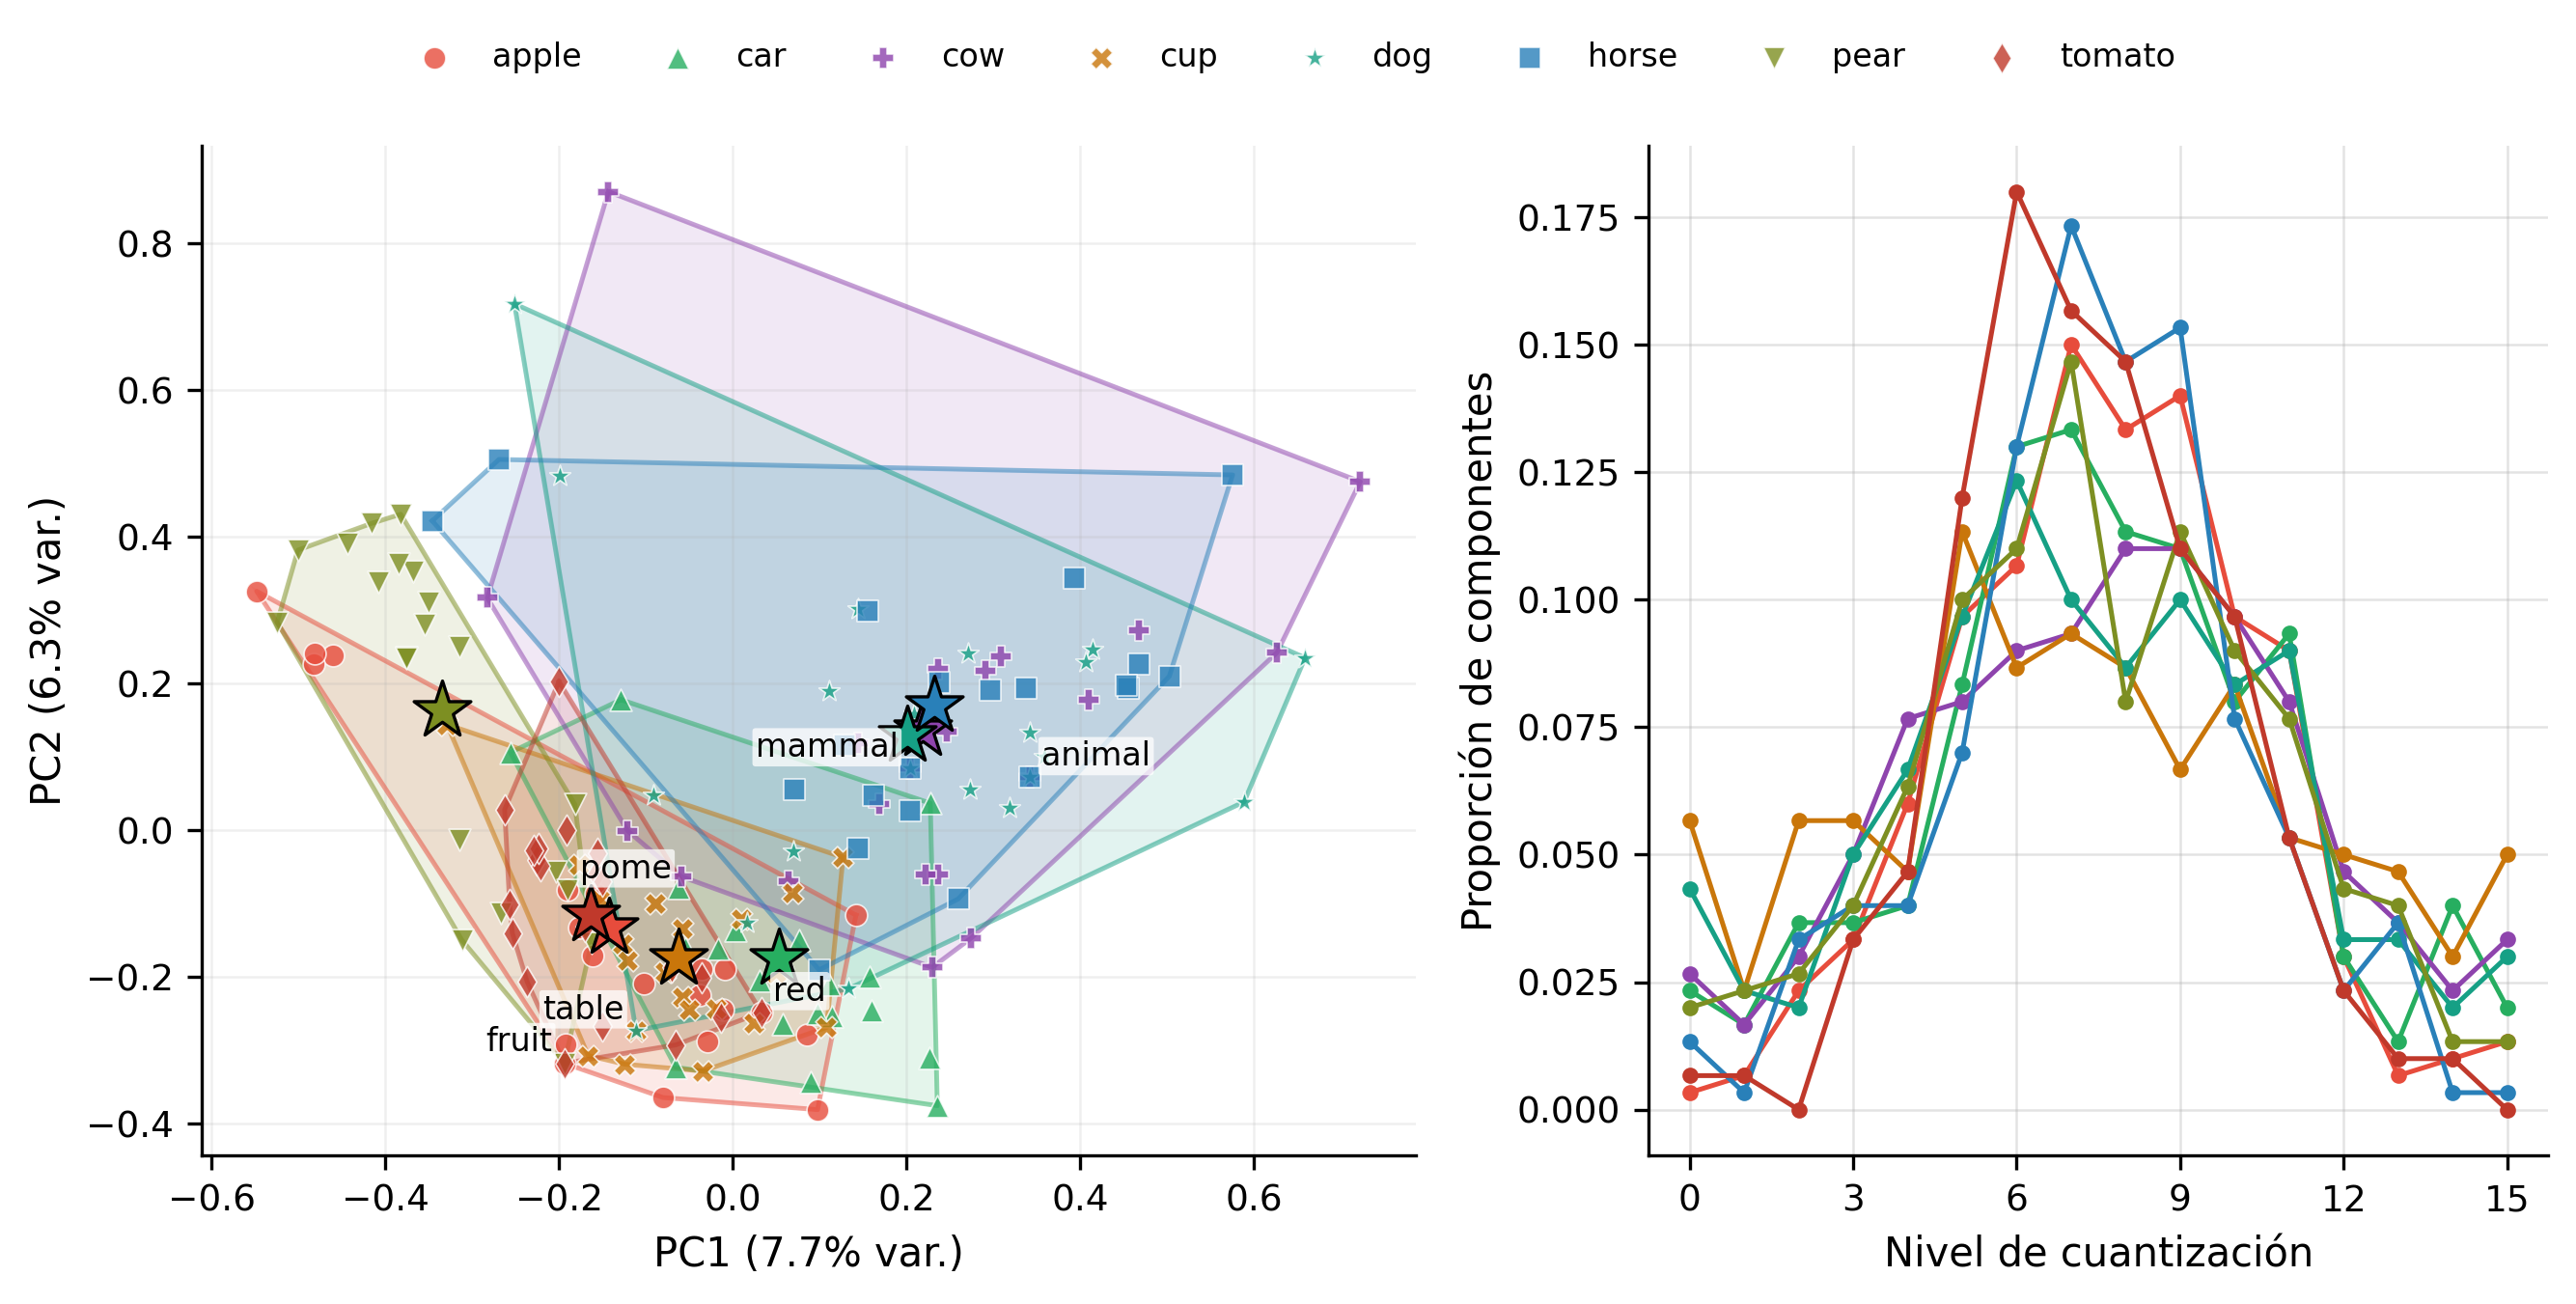
\includegraphics[width=\textwidth]{fig11_semantic_space.png}
    \caption{Espacio semántico de las etiquetas de llenado de las ocho clases (vectores
    fastText del vocabulario de la Sección~\ref{sec:pipeline-semantico}).
    Izquierda: proyección PCA 2D, con la envolvente y el centroide (estrella) de cada
    clase; se rotulan solo las etiquetas que comparten dos o tres clases (\textit{fruit},
    \textit{pome}, \textit{red}, \textit{animal}, \textit{mammal} y \textit{table}).
    Derecha: proporción de las 300 componentes que cae en cada uno de los 16 niveles de
    la cuantización por magnitud, para la etiqueta con el nombre de cada clase.}
    \label{fig:espacio-semantico}
\end{figure}

% ---------------------------------------------------------------
\subsection{La normalización necesaria es B1}
\label{sec:disc-b1}

La lectura B1 del directorio transactivo no corrige un defecto: refleja cómo está
construido el sistema.
Cuando los módulos especialistas acumulan números desiguales de interacciones, la
puntuación cruda del directorio favorece de forma constante al módulo más activo con
independencia del contenido semántico de la consulta.
Dividir entre el conteo normaliza la evidencia a \textit{evidencia por interacción},
comparable entre módulos con historiales de exposición distintos.

La brecha cruda-B1 es de 7.8 puntos con ocho módulos (85.2\% frente a 93.0\%), y la
entropía del directorio es alta incluso con la lectura cruda (2.974 de 3.000 bits): la
\emph{estructura} del directorio está casi balanceada, y el sesgo está en la
\emph{lectura}, donde B1 actúa.
Las condiciones que actúan sobre los síntomas (B2, C, D, E) quedan por debajo de B1, y
la combinación G, que suma correcciones a B1, gana solo medio punto, dentro del ruido
(Tabla~\ref{tab:calibracion}).

% ---------------------------------------------------------------
\subsection{El sesgo hacia un módulo: masa del directorio y léxico compartido}
\label{sec:disc-dominancia}

Con la lectura cruda, \texttt{apple} gana el 20.5\% de las victorias maduras y
\texttt{cow} el 17.0\%: son los dos módulos con más registros en el directorio (186 y
181, frente a 112 de \texttt{horse}).
La puntuación cruda favorece al que más registró (Sección~\ref{sec:disc-b1}); la
lectura B1, que divide entre los registros, deja a \texttt{apple} en 13.8\% (ideal
12.5\%).
Lo que B1 no corrige es léxico.
De los 28 errores que quedan, 9 son \texttt{pear} $\to$ \texttt{apple} y 6
\texttt{horse} $\to$ \texttt{cow}, pares que comparten etiquetas genéricas
(\textit{fruit} y \textit{pome}; \textit{animal} y \textit{mammal}), y \texttt{pear}
se queda en 76\%.
Si el espacio latente del codificador contribuye también al sesgo no se midió en este
trabajo.

% ---------------------------------------------------------------
\subsection{Lectura desde la teoría de memoria transactiva de Wegner}
\label{sec:disc-wegner}

Los resultados de las Secciones~\ref{sec:calibracion}, \ref{sec:formacion},
\ref{sec:capacidad} y~\ref{sec:hemisferio-visual} releen los mecanismos de
Wegner~\cite{wegner1987transactive} con un grupo de ocho miembros:

\begin{itemize}
    \item \textbf{Conocerse cuesta interacción.}
    Con ocho módulos, 10 consultas por dominio dejan la precisión madura en 81.2\%, y
    hace falta el banco completo ($\approx$50 por dominio) para alcanzar el 93.0\%.
    Los errores que quedan caen dentro de pares de módulos que comparten léxico, como
    muestra el punto sobre la comunicación distintiva.

    \item \textbf{El orden de las experiencias afecta la velocidad, no el destino.}
    Todas las condiciones de presentación convergen al mismo directorio: mismos
    conteos, misma entropía.
    En el modelo de Wegner, el directorio se forma anotando quién respondió en cada
    interacción presenciada; aquí cada anotación se suma a las anteriores, así que el
    directorio final depende de \emph{qué} se presenció, y el orden solo decide cuándo
    se vuelve utilizable.

    \item \textbf{La comunicación distintiva forma mejor directorio.}
    Con la lectura B1, \texttt{car}, \texttt{cow}, \texttt{cup} y \texttt{tomato}
    quedan en 98--100\% y \texttt{dog} en 93.9\%; \texttt{pear} (76\%), \texttt{horse}
    (88\%) y \texttt{apple} (88.2\%) pierden hacia la vecina con la que comparten
    etiquetas (Sección~\ref{sec:disc-dominancia}).
    En términos de Wegner, la coordinación de la recuperación funciona en la medida en
    que quien pregunta aporta las señas del dominio: la regla de rescate léxico, que
    solo admite tokens de la consulta como \textit{bark}, \textit{moo} o
    \textit{riding}, sube 21.7 puntos en las 46 consultas que toca
    (Sección~\ref{sec:pipeline-semantico}).

    \item \textbf{El rechazo colectivo se sostiene con ocho dominios.}
    Con siete clases contrarias por módulo, el contenido no acepta ningún falso con un
    latente por imagen, en ninguno de los tamaños de llenado probados, y con las 16
    variantes del experimento 13 acepta 5 de 656 imágenes de prueba, todas entre
    animales (vacas y caballos aceptados por \texttt{dog}, un caballo por
    \texttt{cow}).
    El directorio visual comete dos falsos enrutamientos de 656.
    Es el rechazo de la Sección~\ref{sec:tmt}: lo que ningún módulo reconoce no se
    responde, y los falsos del contenido caen entre animales.
\end{itemize}

% ---------------------------------------------------------------
\subsection{Una memoria por módulo: familiaridad, nombre y daño}
\label{sec:disc-una-memoria}

Con una sola memoria de contenido, el sistema queda hecho solo de asociaciones: la de
contenido (etiqueta con imagen) dentro de cada módulo y la de directorio (pista con
módulo) entre ellos.
Reconocer una pista no consulta un almacén aparte: es leer la asociación.
Es lo que proponen los modelos de emparejamiento global de la psicología, que leen la
familiaridad de un único almacén de huellas~\cite{clark1996global}: preguntarle a la
memoria conjunta si una imagen es familiar es emparejarla con todas las huellas,
cualquiera que sea su etiqueta, y eso es la suma de la ecuación~\eqref{eq:marginal}.

La lesión de la Sección~\ref{sec:una-memoria} separa las dos lecturas: con daño al
azar en la única memoria, el módulo deja de nombrar mucho antes de dejar de reconocer
(Tabla~\ref{tab:lesion}).
El patrón se parece a disociaciones conocidas.
La paciente YR, con una lesión selectiva del hipocampo, reconoce ítems pero falla en
asociaciones entre tipos distintos de información, como caras con nombres
hablados~\cite{mayes2004associative}.
En ratas, la lesión del hipocampo suprime el recuerdo y deja la
familiaridad~\cite{fortin2004recollection}; con la edad, la memoria de asociaciones se
deteriora más que la de ítems~\cite{old2008differential}.
En el cerebro, estas disociaciones suelen atribuirse a estructuras distintas, la corteza
perirrinal para la familiaridad y el hipocampo para unir ítem y
contexto~\cite{eichenbaum2007medial,diana2007imaging}, aunque esa asignación está en
disputa~\cite{squire2007recognition}.
En este sistema la disociación sale de una sola memoria: nombrar exige que cada
coordenada de la imagen deje apoyo en cada coordenada de la etiqueta, mientras que
reconocer suma la evidencia de todas las etiquetas.
Esto no resuelve el debate, pero muestra que la disociación no exige dos almacenes, como
Plaut mostró para la afasia óptica con un solo sistema semántico de especialización
gradual~\cite{plaut2002graded}.

El estado intermedio, reconocer sin poder nombrar, también tiene análogos.
En la afasia óptica, el paciente identifica un objeto por la vista pero no puede
nombrarlo desde ella~\cite{beauvois1982optic}.
En la experiencia de la punta de la lengua, la persona sabe que conoce la palabra y
recupera partes de ella, como la primera letra o el número de sílabas, sin
alcanzarla~\cite{brown1966tip}; y la sensación de saber anticipa con bastante acierto qué
se reconocerá aunque no se haya podido recordar~\cite{hart1965memory}.
En este sistema el estado aparece en cuanto hay datos sin pareja: de 800 imágenes
registradas sin palabra, 78 quedan reconocidas sin nombre (Sección~\ref{sec:una-memoria}).
La lectura de familiaridad las distingue de un rechazo; el protocolo de respuesta
todavía no las usa.
En términos de Wegner~\cite{wegner1987transactive}, es justo el momento en que un miembro
del grupo debería consultar el directorio: sabe que conoce el objeto y necesita a quien
sepa el nombre.
Estas analogías son estructurales, no causales: en los pacientes la asociación existía y
se dañó; en el sistema, con datos sin pareja, nunca se registró.

% ---------------------------------------------------------------
\subsection{Qué aporta la partición frente a una EHAM única}

La comparación de la Sección~\ref{sec:eham-unica} acota lo que aporta la maquinaria
transactiva.
Lo primero es no mezclar: la relación de una EHAM acumula por coordenada y valor, y dos
conceptos distintos comparten valores cuantizados en muchas coordenadas, así que una
memoria con varios dominios mezcla al recordar aunque las palabras difieran.
Partir el contenido evita la mezcla porque el dominio se decide antes de la
recuperación, en el directorio, y no al muestrear la memoria.
Se ve en la fidelidad: la respuesta de la EHAM única queda más lejos de la instancia
real más cercana en todos los cortes (de 4.6 a 6.2 más que el oráculo), sin tendencia
con el contenido.
Y se ve fuera de dominio: la EHAM única acepta más cuanto más contiene (de 2 a 8 de 40
consultas), y el protocolo con doble compuerta acepta 2 en todos los cortes.

La exactitud de clase también mejora, pero poco.
Desde 50 imágenes por clase el protocolo acierta entre 98.3 y 98.8\,\% frente a
96.9--97.6\,\% de la EHAM única, con intervalos separados; con 25 la EHAM única queda
arriba (97.6 frente a 96.9\,\%, con intervalos que se solapan), porque el directorio
todavía enruta peor (95.3\,\% de enrutamiento correcto).

El precio es cobertura y un índice.
El especialista deja sin respuesta al 2.5\,\% de las imágenes de prueba con 200 por
clase, que la EHAM única responde: una de las 80 imágenes porque la contención es
estricta en las 64 coordenadas del latente y otra porque el recuerdo no devuelve palabras.
Es parte del rechazo residual del hemisferio visual (limitación (b)); el protocolo de
esta comparación, que forma su directorio visual sin variantes, responde al 81\,\%.
A eso se suman el error del directorio, de 1.2 a 1.7 puntos de clase desde 50 imágenes
por clase (3.1 con 25), y ocho veces las celdas de memoria: una heteroasociativa por
módulo en lugar de una.

\subsection{Limitaciones}
\label{sec:limitaciones}

\paragraph{(a) Fuga de consultas fuera de dominio en el hemisferio textual.}
Una consulta fuera de dominio que comparte tokens con etiquetas legítimas pasa la
contención textual y llega a algún módulo: la sonda de rechazo deja pasar 2 de 12
(Sección~\ref{sec:proto-completo}), y en el banco de 40 de la comparación con la EHAM
única el directorio acepta 4, dos de ellas (\emph{piano}, \emph{thunderstorm}) hacia un
módulo que no las contiene.
La doble compuerta de contenido (el destino debe contener la consulta, no solo figurar
en el directorio) detiene esas dos y deja al protocolo en 2 de 40 en los cuatro cortes,
tantas como el oráculo; sobre las 171 consultas reservadas no quita ninguna respuesta,
porque las que rechaza (1.5\,\% con 200 imágenes por clase, 2.1\,\% con 25) eran
enrutamientos equivocados que el destino tampoco respondía.
Las dos que quedan las contiene el destino, y ninguna compuerta de contención las
separa de una consulta legítima.
Las alternativas medidas rinden menos (experimento 15, sobre las 171 reservadas): que el
contenido decida entre los tres mejores candidatos del directorio baja el acierto de
96.8 a 93.6\,\%, porque el índice calibrado compara mejor que la activación del
contenido, y abstenerse cuando la diferencia relativa entre las dos mejores
puntuaciones es menor que un umbral $\delta$ quita más de un acierto por cada error
evitado (1.2 con $\delta = 0.05$; 8 con $\delta = 0.5$).

\paragraph{(b) Cobertura visual limitada por la lectura estricta.}
La lectura del directorio visual es estricta ($\xi = 0$): con directorios
perspectivales, los huecos tolerados dependerían de lo que presenció cada módulo.
Para cubrir más, el sistema densifica.
El directorio visual y la recuperación de la heteroasociativa son dos compuertas, y
cada una cede solo con sus propias variantes (experimento 13, sobre las 656 imágenes de
prueba): registrar en el directorio 16 variantes por percepción, en lugar de una, lleva
su aceptación de 73.6 a 96.2\,\%; llenar el contenido con 16 variantes por imagen, en
lugar de 4, lleva la respuesta de la heteroasociativa de 76 a 96\,\%; con las dos, la
cobertura de punta a punta (enrutamiento correcto y respuesta) pasa de 66.5 a
94.5\,\%, con rendimiento decreciente por escalón de variantes.
El sistema usa 16 variantes en las dos y aun así rechaza el 3.5\,\% de las imágenes de
prueba (Sección~\ref{sec:hemisferio-visual}).
Densificar tiene un costo: dos enrutamientos equivocados de 656 y, en el experimento,
cinco imágenes aceptadas por un especialista ajeno, todas entre animales y cuatro de
ellas por \texttt{dog}.
Son vistas nuevas de los mismos objetos, porque la partición es por imagen
(limitación (f)).

\paragraph{(c) Fuga con entradas degeneradas.}
El contenido visual da soporte también a entradas sin estructura, como un lienzo gris
uniforme, porque el codificador las lleva a latentes de norma baja que caen dentro de la
envolvente de los animales (Sección~\ref{sec:hemisferio-visual}); las sondas
estructuradas (ruido, píxeles barajados) sí se rechazan.
Densificar agranda esa fuga: en el experimento 13, con 16 variantes, a la sonda de color
sólido la aceptan tres especialistas en vez de uno y el directorio la enruta.
El umbral de energía (Sección~\ref{sec:percepcion}) cierra el 90\,\% de la fuga
(experimento 14): 137 de las 152 entradas degeneradas aceptadas por una clase ajena caen
bajo $\tau$ (grises de 104 a 168, contrastes $\leq 0.2$ y desenfoques fuertes: todos
los de radio $\geq 12$ y buena parte de los menores).
Como criterio, la norma y la varianza del latente son equivalentes; la varianza de
píxeles no sirve, porque un objeto desenfocado conserva contraste y pierde estructura.
De las 15 entradas que sobreviven, 11 son objetos desenfocados o de bajo contraste que
acepta otra clase (como un \texttt{dog} desenfocado aceptado por \texttt{cow}) y cuatro
son superficies casi uniformes de norma alta (un gris claro, dos colores sólidos y un
gris con ruido); la doble compuerta del punto (a) no las cerraría, porque el contenido
también las acepta.
El umbral cuesta cinco imágenes reales de 3280, todas vistas oscuras de \texttt{cow}:
una percepción de la fase A y cuatro imágenes de prueba que el directorio enrutaba bien
y su contenido aceptaba.

\paragraph{(d) Calidad de la reconstrucción visual.}
Las reconstrucciones son suaves y sin detalle de alta frecuencia
(Figura~\ref{fig:imagen-etiquetas}).
Es un efecto de cómo se entrenó el autocodificador, con un término de reconstrucción MSE y
una cabeza auxiliar de clasificación que solo interviene en el entrenamiento, no en las
decisiones; no es un efecto del sistema de memorias y puede abordarse por separado.
Sobre la reconstrucción en la EAM, véanse la imaginería de Pineda y
Morales~\cite{pineda2023imagery} y la memoria de imágenes naturales de
CIFAR-10~\cite{hernandez2026cifar}, donde entrenar el autocodificador junto con el
clasificador degrada la reconstrucción y por eso se entrenan por separado.

\paragraph{(e) Aprendizaje limitado después de formar el directorio.}
Una vez llena la memoria de contenido y formado el directorio, los módulos dejan de
registrar contenido nuevo: la fase madura enruta y recupera con lo aprendido.
El sistema aún no modela la asignación de información de Wegner (encaminar información
nueva al especialista que corresponde) ni la reorganización de las memorias de contenido
durante la operación madura.

\paragraph{(f) Partición por imagen.}
La partición entre entrenamiento y prueba separa archivos de imagen, no objetos
físicos: los diez objetos de cada clase aportan vistas a ambos lados
(Sección~\ref{sec:dataset}).
Las cifras visuales principales (96.2\% de enrutamiento, evocación de dominio) miden por
tanto generalización a \emph{vistas nuevas de objetos conocidos}.
Con objetos nuevos, la cobertura de punta a punta baja del 95.5 al 89.2\,\%
(Sección~\ref{sec:objetos-nuevos}), y lo que se pierde es respuesta, no acierto: la
envolvente por coordenada cubre a la mayoría de los objetos que no contribuyeron a ella,
rechaza las vistas que no cubre en lugar de enviarlas a otra clase, y la brecha se
concentra en unos pocos objetos, no en clases.
Con diez objetos por clase, ``objeto nuevo'' sigue siendo un objeto de la misma
colección fotografiado en las mismas condiciones; fotos de otro origen son otra
pregunta.

\paragraph{(g) Selección de modelo e hiperparámetro sobre el conjunto de prueba.}
Dos elementos del protocolo se eligieron mirando el conjunto de prueba, por ausencia
de una partición de validación separada: el punto de control del codificador (RMSE
mínimo sobre el conjunto de prueba entre cinco candidatos, Sección~\ref{sec:percepcion})
y las 16 variantes del llenado, adoptadas después de ver el barrido de variantes
(experimento 13), que mide sobre las 656 imágenes de prueba (16 es el mayor valor
probado, no un óptimo ajustado).
La lectura del directorio visual no tiene tolerancia que ajustar ($\xi = 0$,
limitación (b)).
Ambas selecciones son de alcance acotado y ninguna introduce un mecanismo ajeno a las
memorias, pero pueden inflar las cifras visuales reportadas; la corrección (una
partición de validación aparte) es directa y queda pendiente.

\paragraph{(h) Regla de admisión de pistas alineada con el vocabulario propio.}
El rescate de atención léxica (Sección~\ref{sec:pipeline-semantico}) admite tokens
que el filtro gramatical (POS) descarta si figuran en el vocabulario que llenó las
memorias; su efecto medido es de +21.7 puntos sobre las 46 consultas afectadas del
banco (43 de 46 correctas con rescate, 33 sin él).
La regla nunca censura y no decide el ganador, pero decide \emph{quién vota} con un
criterio derivado del conocimiento del propio sistema; un criterio de rescate
independiente del vocabulario (p.\ ej.\ solo la etiqueta POS de diccionario) eliminaría
la alineación al costo medido.

\paragraph{(i) Dependencia de la calidad de la fuente de conocimiento.}
El vocabulario de ConceptNet es asimétrico entre clases, y el techo de las clases de
léxico compartido (\texttt{pear} 76\%, \texttt{horse} 88\%) depende de la
distintividad de las consultas del banco tanto como del vocabulario del módulo.
Este trabajo no midió si enriquecer el vocabulario de una clase lo corrige.

\paragraph{(j) Fragilidad del nombre ante daño.}
La proyección exige que cada coordenada de la imagen deje apoyo en cada coordenada de la
etiqueta, y no tolera ninguna columna vacía.
Destruir al azar el 1\,\% de las celdas de la memoria de contenido deja sin nombre al
92\,\% de las imágenes emparejadas, y el 5\,\% a todas
(Tabla~\ref{tab:lesion}); el reconocimiento, en cambio, sobrevive.

\section{Conclusiones}
\label{sec:conclusiones}

Este trabajo construyó EAM-TMS, un sistema distribuido de memoria transactiva hecho de
Memorias Asociativas Entrópicas ponderadas (W-EAM) y de su extensión heteroasociativa
(EHAM)~\cite{pineda2021entropic,pineda2022weighted,morales2025missing}, y lo estudió en
cinco fases.
Un prototipo de tres módulos sirvió para comprobar que el directorio emerge del uso y
para elegir cómo leerlo.
Después el sistema creció a los ocho módulos de ETH-80, con una memoria heteroasociativa
por módulo, y sobre esa versión se midieron sus propiedades y se integraron la voz y la
cámara.
Las decisiones de enrutamiento y de rechazo no usan clasificadores discriminativos; la
partición del contenido usa las etiquetas de clase, y el codificador visual se entrenó
con una pérdida de clasificación auxiliar, de la que depende el enrutamiento visual.
Del modelo de Wegner, el sistema implementa la actualización del directorio y la
coordinación de la recuperación; la asignación de información la hace la etiqueta.

Cada cifra de este capítulo va con la arquitectura de su fase.
Entre el prototipo y el sistema final cambiaron a la vez el codificador, la cuantización
de las pistas, las memorias por módulo, el banco de consultas y el mediador, de modo que
las cifras de tres módulos no se comparan con las de ocho como un experimento controlado.

\paragraph{Respuesta a la pregunta de investigación.}
\paragraph{Emergencia del directorio (fase 1).}
El directorio emerge de la experiencia con la arquitectura de la fase 1: tres módulos,
cuatro memorias por módulo, cuantización por signo, TME mediador y banco de 80 consultas.
Empieza vacío, y tras una sola interacción la fase madura acierta el 26.25\,\% de las
consultas y rechaza el 72.5\,\%.
A las 13 interacciones acierta el 91.25\,\%, y con las 80 del banco, el 98.75\,\%, con
un rechazo del 1.25\,\%.
La prueba más directa es el orden bloqueado por dominio.
Mientras solo se presentaron consultas de \texttt{apple}, el directorio solo enrutó a
\texttt{apple} y se quedó en el 33.75\,\%, la parte de esa clase en el banco; cruzó el
90\,\% hasta la interacción 67, ya dentro del bloque de \texttt{car}.
El orden intercalado, el barajado y el bloqueado terminan en las mismas cuentas,
[78, 65, 53].
En él queda a quién vio ganar cada pista, y lo que no presenció no lo enruta.
Esta respuesta tiene tres límites.
La curva se midió sobre las mismas 80 consultas que forman el directorio, así que mide
cuánto del banco cubren los tokens ya registrados; el techo lo pone la fase temprana
(98.73\,\% acumulado frente al 98.75\,\% de la madura), y sin la lectura B1 la fase
madura no lo alcanza.
La formación con ocho módulos no repite el umbral: ninguna condición pasa del 90\,\% y
todas terminan en el 81.2\,\% (Sección~\ref{sec:formacion}).

\paragraph{Lectura del directorio (fase 2).}
La lectura elegida en la fase 2 es B1, que divide la evidencia de cada módulo entre su
número de registros más uno.
En el prototipo, sobre las 80 consultas, la lectura cruda deja la fase madura en el
53.75\,\%, porque \texttt{apple}, el módulo con más registros, gana el 78.75\,\% de las
consultas.
B1 la sube al 98.75\,\%, y dividir entre la raíz del número de registros (B2) se queda en
el 75.0\,\%.
La elección se sostuvo con ocho módulos.
Sobre conjuntos fijos de 120 consultas que nunca forman el directorio, B1 supera a la
lectura cruda con todos los tamaños de formación y en todos los sorteos, por 4.5 a 8.8
puntos en promedio, y con ella la fase madura sube del 78.9\,\% con 50 consultas de
formación al 91.0\,\% con 291, frente al 89.7\,\% de la temprana
(Sección~\ref{sec:calibracion-fija}).
Leer el directorio con el principio de tamaño da en ETH-80, donde el registro está
balanceado, las mismas decisiones que B1 salvo una de 656 imágenes y 8 de 411 consultas.
B1 opera fuera de las memorias y corrige un sesgo de la lectura sin tocar lo registrado.
En el sistema de ocho módulos, la lectura cruda le da a \texttt{apple} el 20.5\,\% de las
consultas aunque las cuentas del directorio están casi parejas (2.974 de 3.000 bits), y B1 lo deja
en el 13.8\,\% (Sección~\ref{sec:calibracion}).

\paragraph{Escalado a ocho módulos (fase 3).}
El escalado a los ocho módulos de ETH-80 funciona con una memoria heteroasociativa y dos
directorios por módulo.
La caída del protocolo completo, del 98.75\,\% de la fase madura con tres módulos al
81.2\,\% con ocho, no se puede atribuir al número de módulos, porque en el paso cambiaron
también el codificador, la cuantización, las memorias, el banco y el mediador.
En la arquitectura final, el hemisferio visual enruta el 96.2\,\% de las 656 imágenes de
prueba con dos falsos enrutamientos, y 113 de las 116 imágenes enrutadas entre las 15
primeras de cada clase evocan palabras de su dominio
(Sección~\ref{sec:hemisferio-visual}).
Ante objetos que ningún módulo vio, la cobertura de punta a punta es del 89.2\,\%; con un
codificador reentrenado sin el objeto reservado es del 87.6\,\%, y los falsos
enrutamientos suben de 2 a 136 de 3280 (Sección~\ref{sec:objetos-nuevos}).
Las memorias homoasociativas que antes se llenaban aparte equivalen a lecturas de la
heteroasociativa: con una sola memoria de contenido por módulo, el sistema toma las
mismas decisiones en imagen y casi todas en texto (Sección~\ref{sec:una-memoria}).

Sobre el tamaño hay dos mediciones controladas, las dos con la arquitectura final.
Frente a una sola EHAM con las ocho clases y el mismo contenido, el sistema acierta la
clase igual desde 50 imágenes por clase; con 200, sobre las 171 consultas reservadas,
aciertan el 96.8 y el 96.9\,\% ($p = 0.86$).
La partición compra fidelidad del recuerdo (lo recordado queda 5.4 unidades más cerca de
una instancia real), menos mezcla cuando la pista es compartida (71.4 frente a 51.1\,\% de
clase correcta) y un rechazo que no empeora con el contenido (acepta 2 de 40 consultas
fuera de dominio, y la EHAM única, 8); esa ventaja en el rechazo depende de una segunda
compuerta decidida después de ver esas consultas (limitación (g)).
A cambio, en imagen responde al 81.2\,\% de las imágenes, y la EHAM única al 100\,\%
(Sección~\ref{sec:eham-unica}).
En los 28 pares de clases de ETH-80, una EHAM de dos clases recuerda a 2.54 unidades de
distancia más que el especialista, en promedio, y la de ocho a 5.66, peor en 26 de los 28
pares.
Esa brecha no sigue al solapamiento entre los dos dominios ($\rho = 0.01$), y el error de
clase sí ($\rho = 0.49$, $p = 0.008$).
Mezclar más dominios en una memoria degrada el recuerdo antes que el acierto de clase;
hasta 200 imágenes por clase, la memoria única no llega a un techo en el acierto, y dónde
lo alcanza queda por medir.

Frente a decisores simples sobre los mismos vectores, la memoria no agrega acierto de
clase.
En las 80 consultas del protocolo completo, el voto por tokens del vocabulario, el
centroide y los vecinos más cercanos aciertan entre el 76.0 y el 81.5\,\%, frente al
81.2\,\% del sistema, y en imagen un centroide o un vecino más cercano aciertan de 652 a
655 de las 656 imágenes, frente a 631 (Sección~\ref{sec:lineas-base}).
Agrega un rechazo que en texto no usa umbral, aunque equivale a la pertenencia
al vocabulario, el recuerdo del contenido asociado y decisiones que se leen en los
registros de sus memorias.
Las representaciones deciden la clase: en texto, el léxico que comparten clases vecinas
concentra los errores (\texttt{pear} $\to$ \texttt{apple} 9 y \texttt{horse} $\to$
\texttt{cow} 6 de 28), como en la sobrecarga de pistas de la memoria
humana~\cite{watkins1975buildup}, y en imagen, sin la pérdida de clase del codificador, el
enrutamiento baja al 70.4\,\% (Sección~\ref{sec:codificador-sin-clase}).

\paragraph{Propiedades del sistema escalado (fase 4).}
En el sistema escalado, el directorio funciona como un índice y, leído al revés, como un
registro de lo que sabe cada miembro.
Para enrutar solo cuenta quién ganó cada pista.
Un directorio único para texto e imagen enruta el texto igual que uno separado (96.2\,\%
en los dos), y las dos modalidades no se transfieren nada.
Leído de módulo a pista, el directorio reconstruye el dominio propio y el de los módulos
ajenos que presenció (80 de 80 y 112 de 112), y lo que devuelve es una envolvente del
dominio, de 2.9 a 5.5 veces más lejos de cualquier instancia real que las instancias
entre sí.

Registrar solo lo que cada módulo presencia no le cuesta acierto al grupo.
En imagen, encadenar los directorios parciales iguala al registro compartido (81.9\,\%
con una de cada 64 transmisiones ajenas presenciadas); en texto lo iguala sumar los
puntajes de los módulos conocidos (91.0 frente a 93.6\,\% con una de cada 32).
Cuando falta un especialista, el directorio sigue apuntando a él, de modo que el grupo
pierde la respuesta y conserva la ubicación, como en la pérdida de un miembro que
describe Wegner~\cite{wegner1987transactive}.
Sustituirlo por el segundo mejor responde el 24.5\,\% de las veces y nunca con la clase
correcta, mientras que describirlo con la lectura inversa del directorio responde siempre
y con la clase correcta.
El reconocimiento queda en el especialista, que acepta el 98.3\,\% de las
consultas de su dominio, y un módulo ajeno, el 16.1\,\%.
Estos experimentos de lectura inversa, perspectiva y pérdida de un miembro usan
protocolos anteriores al sistema final, con directorios compartidos o con un directorio
visual formado sin variantes.

Reconocer y recordar se separan dentro de una misma memoria.
La memoria acepta lo que su envolvente cubre, aunque no se parezca a nada visto; el
codificador lleva las entradas sin estructura cerca del origen, ese punto cae en el
soporte de \texttt{horse}, y el umbral de energía $\tau$ cierra 137 de 152 de esas
entradas.
Ante un daño al azar, el módulo deja de nombrar mucho antes de dejar de reconocer: destruir
el 1\,\% de las celdas deja sin nombre al 92\,\% de las imágenes, porque nombrar es una
conjunción sobre todas las coordenadas y reconocer, una suma.
Ese patrón tiene análogos en las personas, como la afasia óptica o la experiencia de la
punta de la lengua (Sección~\ref{sec:disc-una-memoria}).

De una imagen el sistema recupera el dominio con más seguridad que la palabra.
El primer término evocado pertenece al vocabulario de la clase en el 96.0\,\% de las
imágenes, y es el nombre de la clase en el 48.0\,\%.
En objetos nuevos, el color se acierta en el 57.8\,\% frente a una base del 49.5\,\%, y
un atributo visible, como el patrón o el pelo, sale con el valor mayoritario del módulo
en el 98 al 99\,\% de las vistas, de modo que el valor minoritario se acierta del 1 al
6\,\%.
La pertenencia a la clase generaliza; el atributo lo decide la densidad de lo
registrado.

Los límites del rechazo también se midieron.
De 12 consultas fuera de los ocho dominios, la memoria rechaza 10 por contención, y la
contención estricta por coordenada rechaza 23 imágenes que un vecino más cercano
clasifica bien.
El rechazo se probó con consultas de texto y con sondas visuales sintéticas; con
fotografías reales de otras categorías no se midió.

\paragraph{Voz y cámara (fase 5).}
La fase 5 es una demostración de integración, hecha con la versión v5 del sistema: ocho
módulos con tres memorias de contenido por módulo.
Una frase grabada, «Farm animal that gives milk», pasó por el detector de voz, Whisper y
el enrutamiento y llegó a \texttt{cow} en unos 0.6\,s, de los que 336\,ms fueron de
transcripción y 302\,ms de enrutamiento.
La visión analiza un cuadro en 54\,ms con la interfaz a 26 cuadros por segundo, y un
cuadro de la cámara sin ningún objeto de las ocho clases se rechaza.
En simulación, la corrección de color recupera 22, 18 y 15 de 24 imágenes de prueba sin
degradar, con degradación media y con degradación fuerte.
Son mediciones únicas de julio de 2026, sin salida cruda guardada; la frase entró desde
un archivo de audio y no se habló en vivo, y con la cámara física y hojas impresas solo
\texttt{cow} se reconoció de forma fiable.
No hay tasa de error de transcripción ni aciertos de enrutamiento con voz.
Esta fase muestra que la cadena funciona de punta a punta; cuánto acierta está por
medir.

\paragraph{Lo que se sostuvo y lo que cambió.}
La Sección~\ref{sec:creencias} contrasta cada creencia inicial con lo que se encontró.
Se sostuvieron tres decisiones: la lectura normalizada por conteo, elegida con tres
módulos y vigente con ocho; el directorio como índice para enrutar, que el directorio
unificado de texto e imagen confirmó; y la idea de que el acierto lo ponen sobre todo las
representaciones, con el matiz de que el mecanismo tiene límites propios.
La ventaja de la fase madura sobre la temprana cambió, porque venía de evaluar sobre las
consultas que formaron el directorio, y con un conjunto fijo la madura solo alcanza a la
temprana.
También cambió la fidelidad de 10 de 10 del primer prototipo, que contaba dos rechazos
como coincidencias.
Al pasar a ocho módulos, la cuantización por signo de las pistas se reemplazó por una por
magnitud.
Partir el contenido entre especialistas dio fidelidad, menos mezcla y rechazo, con el
mismo acierto de clase que una sola memoria.
Tampoco se sostuvo que todas las decisiones fueran operaciones de memoria, porque la suma
por tokens, B1, el umbral $\tau$ y el rescate léxico operan fuera de ellas
(Sección~\ref{sec:auditoria}).

\paragraph{Trabajo futuro.}
Los siguientes pasos salen de las limitaciones de la Sección~\ref{sec:limitaciones}:
\begin{enumerate}
    \item \textbf{Partición de validación y bancos nuevos} (limitaciones (g) y (l)): elegir el
    punto de control del codificador, el número de variantes, la lectura del directorio y
    las compuertas sin usar el conjunto de prueba, y confirmar las cifras de texto, de
    imagen y fuera de dominio con bancos nuevos, escritos por terceros sin acceso al
    vocabulario, y con una partición reservada sorteada en lugar de la cola de la lista
    de cada clase.
    \item \textbf{Barrido del número de módulos con la arquitectura final}: tomar
    subconjuntos de 2 a 8 módulos de los modelos actuales, sin reentrenar ni volver a
    llenar, porque las memorias de contenido son independientes por módulo, y formar de
    nuevo los directorios.
    Separaría el efecto del número de módulos de los demás cambios del escalado; el
    codificador seguiría siendo el de ocho clases, y habría que declararlo.
    Con los tiempos de las etapas 6 a 8 medidos en septiembre en la segunda laptop, cada
    número de módulos y semilla costaría unos 17 minutos.
    \item \textbf{Pérdida de un miembro con el protocolo final}: repetir el experimento 9
    con directorios perspectivales, una memoria heteroasociativa por módulo y el
    directorio visual de 16 variantes, y fijar con esa corrida cuántas consultas llegan al
    módulo perdido según el número de interacciones.
    \item \textbf{Voz y cámara con cifras}: un banco de frases habladas en vivo, con su
    tasa de error de transcripción y su acierto de enrutamiento; latencias repetidas, con
    su distribución, y un conteo de aciertos con la cámara física y objetos impresos.
    Todo con la arquitectura final y guardando la salida cruda en \texttt{results/}.
    \item \textbf{Asignación de información y aprendizaje en fase madura} (limitación
    (e)): que una imagen o una palabra nueva entre por cualquier módulo y el grupo la
    registre en el especialista que indique su directorio, sin la etiqueta de clase (la
    asignación de información de Wegner); que los módulos sigan registrando después de
    formar el directorio, y que el directorio se reorganice cuando un módulo sale del
    grupo o entra en él.
    \item \textbf{Reconocer sin nombrar como consulta al directorio}
    (Sección~\ref{sec:disc-una-memoria}): cuando un módulo reconoce una imagen pero no
    puede nombrarla, que pregunte el nombre a quien lo sepa, como en el modelo de
    Wegner, en lugar de no responder.
    \item \textbf{Directorios perspectivales en texto y criterio de madurez}
    (Sección~\ref{sec:disc-wegner}): repetir la calibración y la curva de formación con
    directorios perspectivales, medir cuánto convergen entre sí los directorios de los
    módulos y que el paso a la fase madura lo decida un criterio interno, como que la
    información mutua entre dominio y ganador deje de crecer.
    \item \textbf{Fuentes de conocimiento complementarias a ConceptNet} (limitación
    (i)): medir si conocimiento alineado con el lenguaje de las consultas eleva el techo
    de las clases con léxico compartido (\texttt{pear} 76\,\%, \texttt{horse} 88\,\%).
    \item \textbf{Rechazo con imágenes reales de otras categorías}
    (Sección~\ref{sec:disc-lineas-base}): medir cuántas fotografías de objetos ajenos a
    las ocho clases aceptan los directorios visuales y las memorias de contenido, frente
    a los decisores simples sobre los mismos latentes, que no rechazan ninguna; el
    rechazo visual de este trabajo solo se probó con sondas sintéticas.
    \item \textbf{Evocación estricta} (Sección~\ref{sec:hemisferio-visual}): medir la
    evocación de dominio de las 116 imágenes con el criterio estricto, que solo cuenta
    las palabras exclusivas de la clase.
    \item \textbf{Lesión con un nombrar graduado} (limitación (j)): repetir la lesión con
    un nombrar que tolere una fracción de columnas vacías y con un daño difuso, y medir
    si la disociación se mantiene, si aparece la inversa y si las etiquetas evocadas
    derivan hacia las compartidas entre clases.
    \item \textbf{Curva del techo entrópico}: llenar la EHAM única con más clases y más
    contenido que en este trabajo, hasta encontrar dónde cae el acierto de clase, y
    comparar ahí con el reparto entre especialistas.
\end{enumerate}

\bigskip

Las Memorias Asociativas Entrópicas de Pineda y Morales bastan para construir un sistema
distribuido de memoria transactiva de ocho especialistas, bidireccional y con rechazo
explícito, sin clasificadores discriminativos en las decisiones de enrutamiento y
rechazo.
Desde el prototipo de tres módulos el directorio emerge del uso, y la lectura elegida ahí
es la que usa el sistema de ocho.
El mecanismo necesita dos cosas que no salen de él, la normalización por conteo del
directorio y un código en que cada coordenada separe las clases.


% -------------------------------------------------------
% Bibliografía
% -------------------------------------------------------
\bibliographystyle{apalike}
\bibliography{referencias}

\end{document}
